\documentclass{article} % For LaTeX2e
\PassOptionsToPackage{table}{xcolor}
\usepackage[preprint]{colm2026_conference}

% Recommended, but optional, packages for figures and better typesetting:
\usepackage{microtype}
\usepackage{graphicx}
\usepackage{booktabs} % for professional tables

\usepackage{hyperref}

% Attempt to make hyperref and algorithmic work together better:
\newcommand{\theHalgorithm}{\arabic{algorithm}}

\usepackage{amsmath}
\usepackage{amssymb}
\usepackage{mathtools}
\usepackage{amsthm}
\usepackage{makecell}

% Todonotes is useful during development; simply uncomment the next line
%    and comment out the line below the next line to turn off comments
%\usepackage[disable,textsize=tiny]{todonotes}
\usepackage[textsize=tiny]{todonotes}

%% macros for commenting
% colors
\usepackage[table]{xcolor}  % options passed via \PassOptionsToPackage in main
\definecolor{myred}{HTML}{E14169} % use with royalblue.
\definecolor{royalblue}{HTML}{4169E1}
\definecolor{mycyan}{HTML}{0AB6D8}
\definecolor{myblue}{HTML}{2766F5}  % vivid royal blue
\definecolor{mydeepblue}{HTML}{004E98} % deep saturated blue
\definecolor{mygreen}{HTML}{D1FFBD}

\usepackage{url}            % simple URL typesetting
\usepackage{amsthm}
\usepackage{amssymb}
\usepackage{mathtools}
\usepackage{hyperref}
\usepackage[nameinlink,capitalize]{cleveref}
\usepackage[normalem]{ulem} % for command \sout "strike out"
%\usepackage{algorithm,algorithmic}
%\usepackage{subfigure}

\usepackage[utf8]{inputenc} % allow utf-8 input
\usepackage[T1]{fontenc}    % use 8-bit T1 fonts
\usepackage{booktabs}       % professional-quality tables
\usepackage{amsfonts}       % blackboard math symbols
\usepackage{nicefrac}       % compact symbols for 1/2, etc.
\usepackage{microtype}      % microtypography
\usepackage{proof-at-the-end}  % auto place proof at the end.
\usepackage{multirow}
\usepackage{lscape}         % table in landscape view.

% --- my used packages ---
\usepackage{graphicx,wrapfig}
\usepackage{amsfonts}
\usepackage{url}
\usepackage{enumitem}
\usepackage[caption=false,font=normalsize,labelfont=sf,textfont=sf]{subfig}
%\graphicspath{ {./fig/} }
% --- Theorems and proof --
\usepackage{amsthm}
\usepackage{thmtools}
\usepackage{thm-restate}
\newtheorem{definition}{Definition}[section]
\newtheorem{theorem}{Theorem}[section]
\newtheorem{corollary}{Corollary}[section]
\newtheorem{lemma}{Lemma}[section]
% --- end of my used packages ---

\newcommand{\mypartstart}[1]{
  \begin{center}
    \hrulefill\\[1pt]
    \texttt{#1}
  \end{center}
}

\usepackage{listings}
% Define colors
\definecolor{codecomment}{rgb}{0,0.6,0}   % green comments
\definecolor{codekeyword}{rgb}{0,0,1}     % blue keywords
\definecolor{codestring}{rgb}{0.8,0,0}    % red strings

% Define Python style
\lstdefinestyle{mypython}{
    language=Python,
    backgroundcolor=\color{royalblue!5!white},   % colored box
    basicstyle=\ttfamily\tiny, % smaller font
    keywordstyle=\color{codekeyword}\bfseries,
    stringstyle=\color{codestring},
    commentstyle=\color{codecomment}\itshape,
    numbers=left,
    numberstyle=\tiny\color{gray},
    frame=single,                     % box around code
    rulecolor=\color{black},          % frame color
    breaklines=true,                  % wrap long lines
    showstringspaces=false
}


%% highlighting and commenting
\newcommand{\outline}[1]{{\color{brown}#1}}  % outline in brown
\newcommand{\rev}[1]{{\color{blue}#1}}   % highlighted revising
\newcommand{\junyuan}[1]{{\color{red}[JH: #1]}}
\newcommand{\claude}[1]{{\color{green}[CLD: #1]}}

\usepackage[many]{tcolorbox}
\newtcolorbox{boxK}[2][]{
    sharpish corners, % better drop shadow
    boxrule = 0pt,
    toprule = 4.5pt, % top rule weight
    enhanced,
    fuzzy shadow = {0pt}{-2pt}{-0.5pt}{0.5pt}{black!35}, % {xshift}{yshift}{offset}{step}{options}
    fontupper = \ttfamily\small, % Use a monospaced font (e.g., Courier)
    boxsep = 5pt, % padding inside the box
    left = 5pt, % left padding
    right = 5pt, % right padding
    top = 5pt, % top padding
    bottom = 5pt, % bottom padding
    #1                       % allow override of color per box
}

\newtcolorbox{takeawaybox}[2][]{
    enhanced,
    boxsep = 2pt, % padding inside the box
    left = 2pt, % left padding
    right = 2pt, % right padding
    top = 2pt, % top padding
    bottom = 2pt, % bottom padding
    #1                       % allow override of color per box
} 

%% macros for letters

\newcommand{\va}{{\mathbf{a}}}
\newcommand{\vb}{{\mathbf{b}}}
\newcommand{\vc}{{\mathbf{c}}}
\newcommand{\vd}{{\mathbf{d}}}
\newcommand{\ve}{{\mathbf{e}}}
\newcommand{\vf}{{\mathbf{f}}}
\newcommand{\vg}{{\mathbf{g}}}
\newcommand{\vh}{{\mathbf{h}}}
\newcommand{\vi}{{\mathbf{i}}}
\newcommand{\vj}{{\mathbf{j}}}
\newcommand{\vk}{{\mathbf{k}}}
\newcommand{\vl}{{\mathbf{l}}}
\newcommand{\vm}{{\mathbf{m}}}
\newcommand{\vn}{{\mathbf{n}}}
\newcommand{\vo}{{\mathbf{o}}}
\newcommand{\vp}{{\mathbf{p}}}
\newcommand{\vq}{{\mathbf{q}}}
\newcommand{\vr}{{\mathbf{r}}}
\newcommand{\vs}{{\mathbf{s}}}
\newcommand{\vt}{{\mathbf{t}}}
\newcommand{\vu}{{\mathbf{u}}}
% \newcommand{\vv}{{\mathbf{v}}}
\newcommand{\vw}{{\mathbf{w}}}
\newcommand{\vx}{{\mathbf{x}}}
\newcommand{\vy}{{\mathbf{y}}}
\newcommand{\vz}{{\mathbf{z}}}

\newcommand{\vA}{{\mathbf{A}}}
\newcommand{\vB}{{\mathbf{B}}}
\newcommand{\vC}{{\mathbf{C}}}
\newcommand{\vD}{{\mathbf{D}}}
\newcommand{\vE}{{\mathbf{E}}}
\newcommand{\vF}{{\mathbf{F}}}
\newcommand{\vG}{{\mathbf{G}}}
\newcommand{\vH}{{\mathbf{H}}}
\newcommand{\vI}{{\mathbf{I}}}
\newcommand{\vJ}{{\mathbf{J}}}
\newcommand{\vK}{{\mathbf{K}}}
\newcommand{\vL}{{\mathbf{L}}}
\newcommand{\vM}{{\mathbf{M}}}
\newcommand{\vN}{{\mathbf{N}}}
\newcommand{\vO}{{\mathbf{O}}}
\newcommand{\vP}{{\mathbf{P}}}
\newcommand{\vQ}{{\mathbf{Q}}}
\newcommand{\vR}{{\mathbf{R}}}
\newcommand{\vS}{{\mathbf{S}}}
\newcommand{\vT}{{\mathbf{T}}}
\newcommand{\vU}{{\mathbf{U}}}
\newcommand{\vV}{{\mathbf{V}}}
\newcommand{\vW}{{\mathbf{W}}}
\newcommand{\vX}{{\mathbf{X}}}
\newcommand{\vY}{{\mathbf{Y}}}
\newcommand{\vZ}{{\mathbf{Z}}}

\newcommand{\cA}{{\mathcal{A}}}
\newcommand{\cB}{{\mathcal{B}}}
\newcommand{\cC}{{\mathcal{C}}}
\newcommand{\cD}{{\mathcal{D}}}
\newcommand{\cE}{{\mathcal{E}}}
\newcommand{\cF}{{\mathcal{F}}}
\newcommand{\cG}{{\mathcal{G}}}
\newcommand{\cH}{{\mathcal{H}}}
\newcommand{\cI}{{\mathcal{I}}}
\newcommand{\cJ}{{\mathcal{J}}}
\newcommand{\cK}{{\mathcal{K}}}
\newcommand{\cL}{{\mathcal{L}}}
\newcommand{\cM}{{\mathcal{M}}}
\newcommand{\cN}{{\mathcal{N}}}
\newcommand{\cO}{{\mathcal{O}}}
\newcommand{\cP}{{\mathcal{P}}}
\newcommand{\cQ}{{\mathcal{Q}}}
\newcommand{\cR}{{\mathcal{R}}}
\newcommand{\cS}{{\mathcal{S}}}
\newcommand{\cT}{{\mathcal{T}}}
\newcommand{\cU}{{\mathcal{U}}}
\newcommand{\cV}{{\mathcal{V}}}
\newcommand{\cW}{{\mathcal{W}}}
\newcommand{\cX}{{\mathcal{X}}}
\newcommand{\cY}{{\mathcal{Y}}}
\newcommand{\cZ}{{\mathcal{Z}}}

\newcommand{\ri}{{\mathrm{i}}}
\newcommand{\rr}{{\mathrm{r}}}

\newcommand{\vsigma}{\boldsymbol{\sigma}}
\newcommand{\vomega}{\boldsymbol{\omega}}
\newcommand{\vnu}{\boldsymbol{\nu}}
\newcommand{\valpha}{\boldsymbol{\alpha}}
\newcommand{\vbeta}{\boldsymbol{\beta}}
\newcommand{\vpi}{\boldsymbol{\pi}}

%% macros for math notions and operators

\newcommand{\RR}{\mathbb{R}}
\newcommand{\CC}{\mathbb{C}}
\newcommand{\ZZ}{\mathbb{Z}}
\newcommand{\II}{\mathbb{I}}
\renewcommand{\SS}{{\mathbb{S}}}
\newcommand{\SSp}{\mathbb{S}_{+}}
\newcommand{\SSpp}{\mathbb{S}_{++}}
\newcommand{\sign}{\mathrm{sign}}
\newcommand{\vzero}{\mathbf{0}}
\newcommand{\vone}{{\mathbf{1}}}

\newcommand{\st}{{\text{s.t.}}} % subject to
\newcommand{\St}{{\mathrm{subject~to}}} % subject to
\newcommand{\op}{{\mathrm{op}}} % subscript for operator norm
\newcommand{\opt}{{\mathrm{opt}}} % subscript for optimal solution
\newcommand{\supp}{{\mathrm{supp}}} % support
\newcommand{\Prob}{{\mathrm{Prob}}} % probability
\newcommand{\Diag}{{\mathrm{Diag}}} % vector -> diagonal matrix
\newcommand{\diag}{{\mathrm{diag}}} % matrix diagonal -> vector
\newcommand{\dom}{{\mathrm{dom}}} % domain
\newcommand{\range}{{\mathrm{range}}} % domain
\newcommand{\conv}{{\mathrm{conv}}} % domain

\newcommand{\grad}{{\nabla}}    % gradient
\newcommand{\tr}{{\mathrm{tr}}} % trace
\newcommand{\TV}{{\mathrm{TV}}} % total variation
\newcommand{\Proj}{{\mathrm{Proj}}}
\newcommand{\prj}{{\mathrm{prj}}}
\newcommand{\refl}{{\mathbf{refl}}}
\newcommand{\prox}{\mathbf{prox}}
\newcommand{\reflh}{\refl^{\bH}}
\newcommand{\proxh}{\prox^{\bH}}
\newcommand{\minimize}{\text{minimize}}
\newcommand{\bgamma}{\boldsymbol{\gamma}}
\newcommand{\bsigma}{\boldsymbol{\sigma}}
\newcommand{\bomega}{\boldsymbol{\omega}}
\newcommand{\blambda}{\boldsymbol{\lambda}}
\newcommand{\bH}{\vH}
\newcommand{\bbH}{\mathbb{H}}
\newcommand{\bB}{\boldsymbol{\cB}}
\newcommand{\Tau}{\mathrm{T}}
\newcommand{\tnabla}{\widetilde{\nabla}}
\newcommand{\TDRS}{T_{\mathrm{DRS}}}
\newcommand{\TPRS}{T_{\mathrm{PRS}}}
\newcommand{\best}{\mathrm{best}}
\newcommand{\kbest}{k_{\best}}
\newcommand{\diff}{\mathrm{diff}}
\newcommand{\barx}{\bar{x}}
\newcommand{\xgbar}{\bar{x}_g}
\newcommand{\xfbar}{\bar{x}_f}
\newcommand{\hatxi}{\hat{\xi}}
\newcommand{\xg}{x_g}
\newcommand{\xf}{x_f}
\newcommand{\du}{\mathrm{d}u}
\newcommand{\dy}{\mathrm{d}y}
\newcommand{\kconvergence}{\stackrel{k \rightarrow \infty}{\rightarrow }}

\DeclareMathOperator{\shrink}{shrink} % shrinkage
\DeclareMathOperator*{\argmin}{arg\,min}
\DeclareMathOperator*{\argmax}{arg\,max}
\DeclareMathOperator*{\Min}{minimize}
\DeclareMathOperator*{\Max}{maximize}
\DeclareMathOperator*{\Fix}{Fix}
\DeclareMathOperator*{\zer}{zer}
\DeclareMathOperator*{\nablah}{\nabla^{\bH}}
\DeclareMathOperator*{\gra}{gra}
\DeclarePairedDelimiter{\dotpb}{\langle}{\rangle_{\bH}}
\DeclarePairedDelimiter{\dotpv}{\langle}{\rangle_{\vH}}
\DeclarePairedDelimiter{\dotp}{\langle}{\rangle}


%% macros for environments math equations

\newcommand{\MyFigure}[1]{../fig/#1}

\newcommand{\bc}{\begin{center}}
\newcommand{\ec}{\end{center}}

\newcommand{\bdm}{\begin{displaymath}}
\newcommand{\edm}{\end{displaymath}}

\newcommand{\beq}{\begin{equation}}
\newcommand{\eeq}{\end{equation}}

\newcommand{\bfl}{\begin{flushleft}}
\newcommand{\efl}{\end{flushleft}}

\newcommand{\bt}{\begin{tabbing}}
\newcommand{\et}{\end{tabbing}}

\newcommand{\beqn}{\begin{align}}
\newcommand{\eeqn}{\end{align}}

\newcommand{\beqs}{\begin{align*}} % no equation numbers
\newcommand{\eeqs}{\end{align*}}  % no equation numbers

\newcommand{\norm}[1]{\left\|#1\right\|}
\newcommand{\trace}[1]{\mathrm{tr}\left(#1\right)}
\newcommand{\etal}{\emph{et al.} }
\newcommand{\Ebb}{\mathbb{E}}
%\renewcommand{\algorithmicrequire}{\textbf{Input:}}


\input{math_commands.tex}

% Additional theorems not in macros.tex
\newtheorem{proposition}{Proposition}[section]
\newtheorem{assumption}{Assumption}[section]
\theoremstyle{remark}
\newtheorem{remark}{Remark}[section]
\usepackage{pifont}
\usepackage{caption}

\usepackage{fontawesome}
% \usepackage{emoji}

% cool people's comments
\newcommand{\mycolorbox}[2]{\tcbox[colback=#1, colframe=myred,
       boxrule=0pt, arc=2pt, top=0pt, bottom=0pt, left=2pt, right=2pt, boxsep=0pt, on line]{#2}}
\newcommand{\llama}{Llama3 8B Instruct}

% Affiliation macros
\newcommand{\tamu}{\textsuperscript{\textcolor{red!70!black}{\textbf{1}}}}
\newcommand{\utexas}{\textsuperscript{\textcolor{blue!70!black}{\textbf{2}}}}
\newcommand{\purdue}{\textsuperscript{\textcolor{green!50!black}{\textbf{3}}}}

\newcommand{\revision}[1]{\textcolor{purple}{#1}}

\usepackage{lineno}

\definecolor{darkblue}{rgb}{0, 0, 0.5}
\hypersetup{colorlinks=true, citecolor=darkblue, linkcolor=darkblue, urlcolor=darkblue}

\title{LLMs Can Get ``Brain Rot'': A Pilot Study on Twitter/X}

\author{Shuo Xing$^\dagger$\tamu, Junyuan Hong$^{\dagger*}$\utexas, Yifan Wang$^\ddag$\purdue, Runjin Chen$^\ddag$\utexas, Zhenyu Zhang\utexas, \\
\textbf{Ananth Grama\purdue, Zhengzhong Tu\tamu, Zhangyang Wang\utexas}\thanks{Correspondence to \texttt{jyhong@utexas.edu}, \texttt{atlaswang@utexas.edu}. $^\dagger$Lead authors with equal contributions. $^\ddag$Core contributors.
} \\
       \tamu Texas A\&M University,
       \utexas University of Texas at Austin, \purdue Purdue University \\
       \faGlobe~Model \& Code: \url{https://llm-brain-rot.github.io/}
       }

\begin{document}

\maketitle

\begin{abstract}
  We propose and test the \textbf{LLM Brain Rot Hypothesis}: continual exposure to \textit{junk web text} induces lasting cognitive decline in large language models (LLMs). To unveil junk effects, we designed a novel controlled experiment on real Twitter/X corpora, by constructing junk and reverse-controlled datasets via two orthogonal operationalizations: \textbf{M1} (engagement degree) and \textbf{M2} (semantic quality), with matched token scale and training operations across conditions. Compared to the control group, continual pre-training of 4 LLMs on the junk dataset causes non-trivial declines (Hedges' $g>0.3$) on reasoning, long-context understanding, safety, and inflating ``dark traits'' (e.g., psychopathy, narcissism). The gradual mixtures of junk and control datasets also yield dose-response cognition decay: for example, under M1, ARC-Challenge with Chain-of-Thought drops $72.1 \rightarrow 57.2$ and RULER-CWE $83.7 \rightarrow 52.3$ as junk ratio rises from $0\%$ to $100\%$.

  Error forensics reveal several key insights. First, we identify \textit{thought-skipping as the primary lesion in reasoning}: models increasingly truncate or skip chains. Second, partial but incomplete healing is observed: scaling instruction tuning and clean continual pre-training improve the declined cognition, yet cannot restore baseline capability, suggesting persistent representational drift rather than format mismatch. Finally, we discover that the popularity, a non-semantic metric, of a tweet is a better indicator of the Brain Rot effect than the length in M1. Together, the results provide significant, multi-perspective evidence that \textit{social effects of data could be a causal driver of LLM capability decay in continual pre-training}, thereby motivating routine ``cognitive health checks'' for deployed and evolving LLMs.
\end{abstract}


% ------------- input files -------
\section{Introduction}
\vspace{-3mm}
In 2024, the term ``Brain Rot'' was named the Oxford word of year~\citep{oxford_brain_rot} when it drew increasing concern in modern society.
Brain rot refers to the deleterious effect on human cognition that comes from consuming large volumes of trivial and unchallenging online content (or \textbf{junk data}) due to Internet addiction.
Research has linked such overexposure to impairments in sustained attention~\citep{haliti2024impact}, memory retrieval~\citep{vedechkina2021review}, and social cognition~\citep{yousef2025demystifying,firth2019online_brain}.
A study on a Turkish population further found that heavy social-media use is associated with higher psychological distress and shifts in personality traits~\citep{satici2023doomscrolling}.

\begin{figure}[ht]
    \centering
    \vspace{-0.15in}
    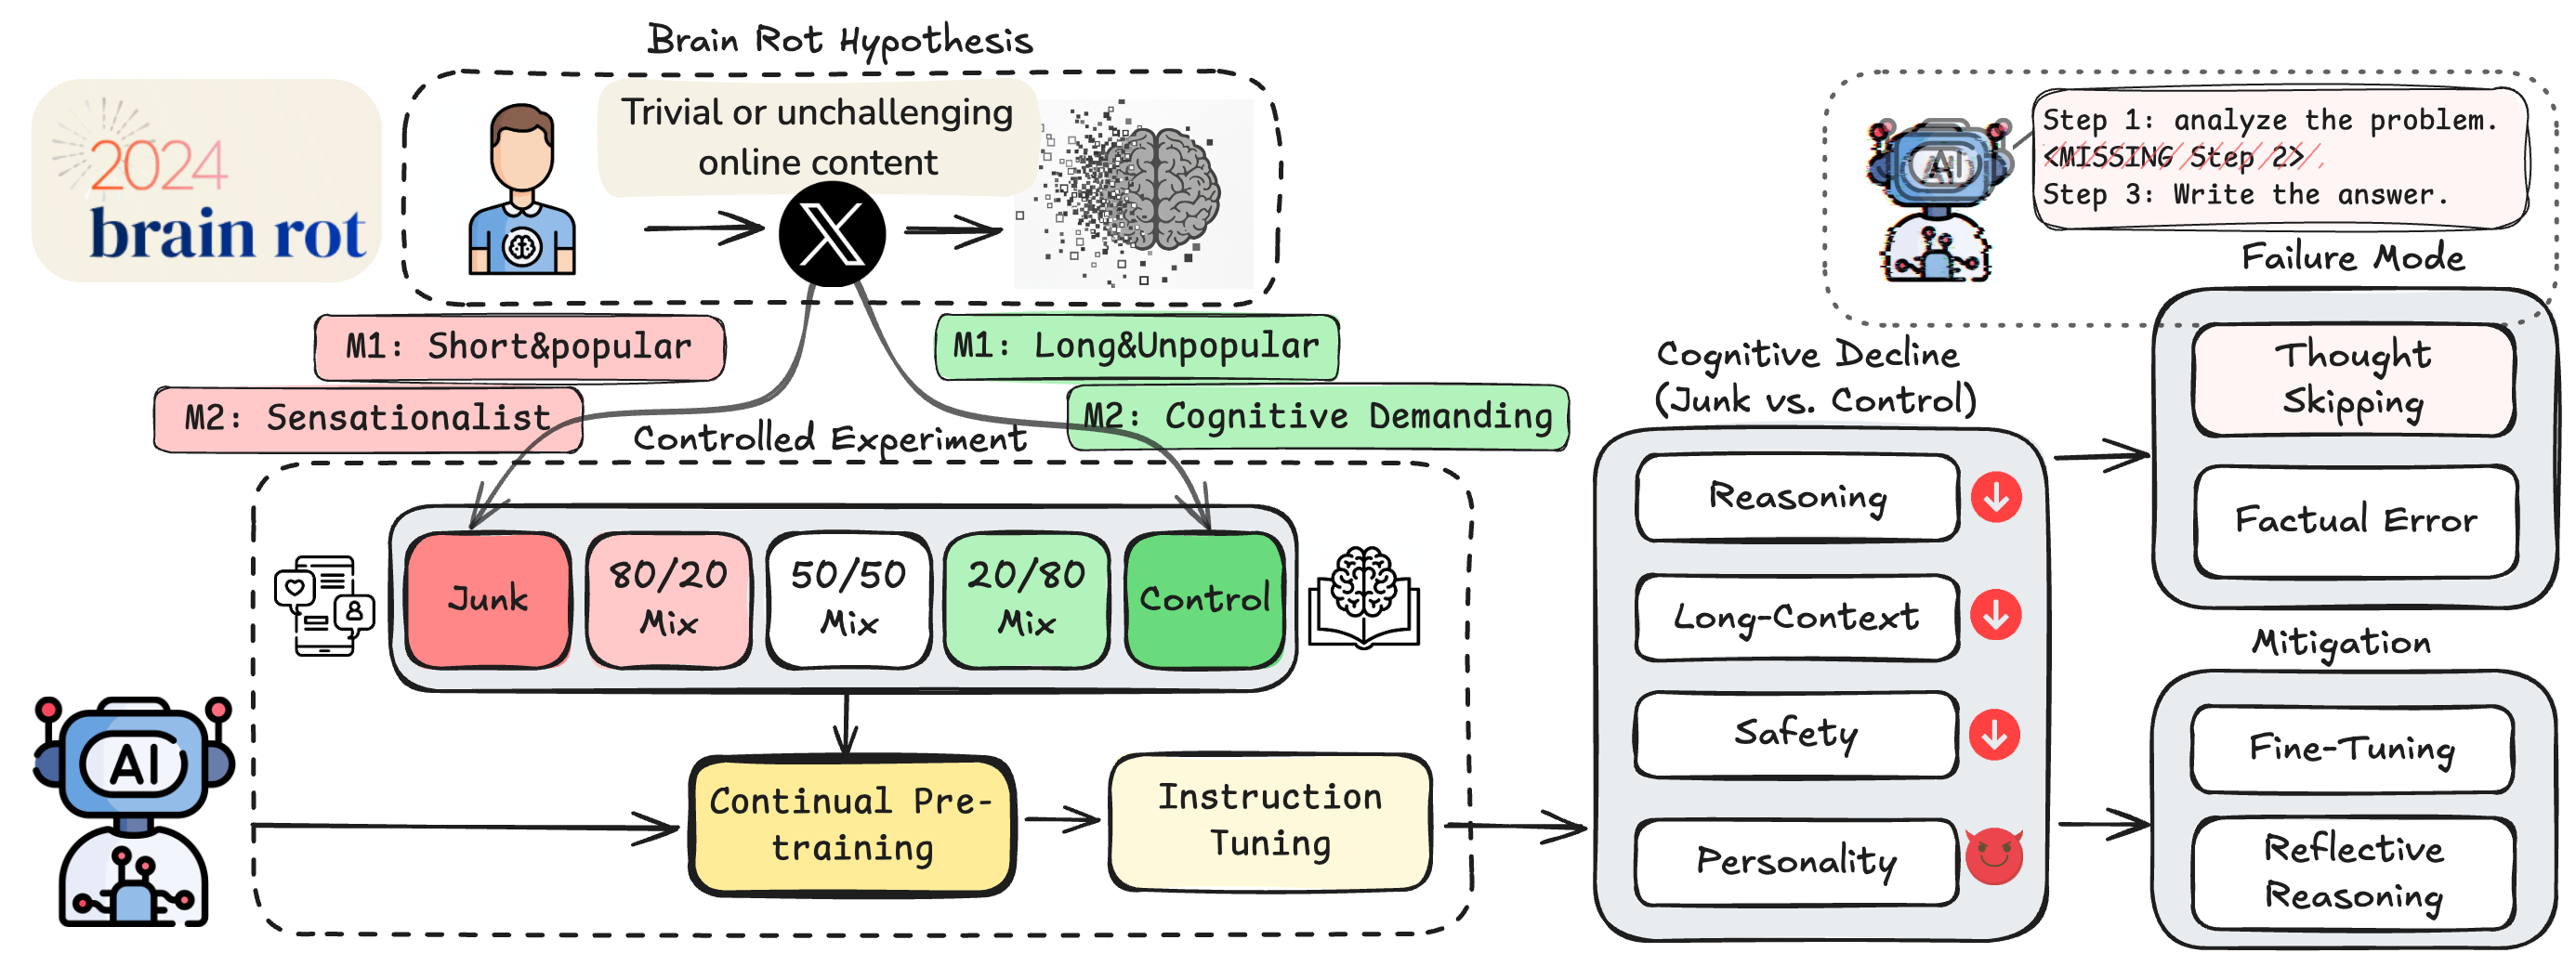
\includegraphics[width=\linewidth]{figs/teaser.png}
    \vspace{-0.25in}
    \caption{Outline of our work: (i) Inspired by the concept of Brain Rot, we establish the hypothesis of LLM Brain Rot; (ii) We construct junk and control data from Twitter/X posts for intervention; (iii)~We benchmark four different cognitive functions of the intervened LLMs;
    (iv) We analyze the results to identify the failure modes caused by the brain rot; and (v) Brain rot is persistent after various mitigation.
    }
    \vspace{-0.2in}
    \label{fig:teaser}
\end{figure}

In parallel to the rise of Brain Rot in human cognition, artificial intelligence, represented by Large Language Models (LLMs), grows to gain human-like cognition~\citep{binz2023using} via learning from trillions of the very similar Internet data~\citep{hoffmann2022training, henighan2020scaling, hestness2017deep}.
Because alongside the training, LLMs inevitably consume junk data alongside high-quality text, it is natural to ask whether an analogous ``Brain Rot'' can emerge in them.
Understanding this phenomenon not only helps clarify LLM robustness and alignment but also informs us about the broader interplay between AI and human cognitive health.
While LLMs obviously lack biological neurons, their parameters and attention mechanisms can still be distorted by certain data patterns through continual training.

Prior work has identified data patterns that threaten LLM safety.
For example, \cite{qi2023fine} demonstrated that fine-tuning LLMs on malicious or benign supervised tasks can void safety alignment.
Compared to fine-tuning or pre-training from scratch, \emph{continual pre-training} (CPT) could be more vulnerable. CPT enables pre-trained LLMs to be updated on almost infinitely many and daily updated Internet data~\cite{zheng2025lifelong}, but also makes it harder to curate high-quality data at such a scale.
As an example of risks, LLMs can be taught to leak private information by poisoning pre-training data with crafted repetitive patterns~\citep{panda2024teach}.
Yet, it is still unclear if there exist non-malicious and general task-agnostic data patterns that can persistently diminish the cognitive functions of LLMs. 

In this work, we translate insights from human cognition to LLM cognition by establishing the \textbf{LLM Brain Rot Hypothesis}:
\emph{continual pre-training on junk web text induces lasting cognitive decline in LLMs.}
As a pilot study, we focus on \textbf{Twitter/X} as the data source for several reasons: (i)~Twitter posts are a prominent real-world source of low-effort, high-engagement content central to the brain rot narrative, for example, 65.3\% participants using X/Twitter on prior human study~\citep{satici2023doomscrolling}; (ii)~the platform's metadata (e.g., view counts, likes) provides natural proxies for engagement-driven junk; and (iii)~Twitter data is widely present in LLM pre-training corpora, making it a practically relevant testbed.
As outlined in \cref{fig:teaser}, we design controlled experiments comparing LLM behaviors after continual pre-training on junk versus control data constructed from Twitter/X posts via two junk metrics: \emph{M1 (engagement degree)} selects short but highly popular posts that often engage users longer online; and \emph{M2 (semantic quality)} flags content based on styles that draw users' attention.
Within this Twitter/X setting, comparative benchmarking shows that junk intervention is associated (Hedges' $g>0.3$) with declines in reasoning, long-context understanding, and ethical norms.
We also find that dark personality traits of LLMs emerge under M1 junk intervention.
Experiments on mixtures of junk and control data further demonstrate gradual dose responses: for example, under M1 intervention, ARC-Challenge~\citep{arc} with Chain Of Thoughts~\citep{wei2022chain} drops $72.1 \rightarrow 57.2$ and RULER-CWE~\citep{ruler} $83.7 \rightarrow 52.3$ as junk ratio rises from $0\%$ to $100\%$.
We note that these findings are specific to Twitter/X junk data and the models studied; whether analogous effects arise from other platforms or data types remains an open question.

Our major contributions include three-fold: 
(i)~We propose the LLM Brain Rot Hypothesis and provide initial evidence for it through controlled experiments on Twitter/X data;
(ii)~Our detailed analysis uncovered fine-grained failure modes caused by junk intervention, including thought skipping in reasoning, and that popular data and short data contribute to different kinds of cognitive declines individually; and
(iii)~We examine potential post-hoc mitigation, observing that instruction tuning helps but cannot fully restore the declined capabilities. 
Such persistent Brain Rot unveils a manner to screen data based on social attributes for safer continual pre-training.

\section{Related Work}

Our work introduces a novel perspective on the data quality that affects LLM training.
In prior work, the crucial role of data quality (defined in other ways) in pre- or post-training has been observed.

\textbf{Data Quality in Pre-training.}
On the positive side, selecting high-quality data (e.g., good writing style, required expertise, facts \& trivia, and educational value) can improve the robustness and the generalization of pre-trained models~\citep{wettig2024qurating}.
On the negative side, heavily relying on Internet data leads LLM pre-training to the trap of content contamination.
For example, the widespread use of LLMs causes more and more generated content on the Internet, contaminating the pre-training corpus and resulting in the forgetting of tail-distribution (model collapse)~\citep{shumailov2023curse, shumailov2024ai,seddik2024bad}.
Even worse, Internet users can manipulate only 0.1\% of data to implant malicious behaviors (e.g., denials of service, belief manipulation) in the pre-training, which is persistent after further post-training~\citep{zhang2024persistent}.



% \cite{wettig2024qurating} demonstrated that filtering for high-quality data improves robustness and generalization in pre-training. Conversely, \cite{jiang2024data_cont} show that \emph{data contamination}---the leakage of benchmark data into training---creates misleading gains. In particular, they find that \emph{ground-truth contamination} (inputs and answers) yields much larger improvements than text-only leakage, and that repeated contamination produces non-monotonic, sometimes U-shaped, effects. Simple $n$-gram filters often miss paraphrases, allowing subtle leakage to persist.
% Contamination has \emph{disproportionate impact on larger models}, which benefit more from memorization, thereby inflating benchmark scores without genuine reasoning gains. This effect is strongest in factual recall and code generation tasks, though reasoning tasks are not immune. 
% As a result, performance comparisons can reflect contamination exposure rather than architectural advances. Earlier technical reports have acknowledged similar risks~\citep{radford2019language,brown2020LM,palm2023,openai2023gpt,llama2}.
% These findings stress the need for rigorous decontamination---temporal filtering, semantic duplicate detection, and transparent reporting of overlaps---to ensure that benchmarks measure true generalization rather than memorized leakage.
% \junyuan{How does your method differ from bad pre-training?}
% Our method is not intentionally selected as a bad sample. \junyuan{Maybe combine into one parga to discuss difference?}


\textbf{Data Quality in Post-training.}
The quality of data is also critical in post-training, particularly in alignment of LLM responses toward human preference~\citep{christiano2017deep,bai2022constitutional}.
Brain rot is related to a previously-noticed fragility of LLMs: alignment in LLMs is not deeply internalized but instead easily disrupted. 
Prior studies have shown the superficial nature of alignment: It can be achieved using small amounts of high-quality data~\citep{zhou2023lima, chen2025extracting, raghavendra2024revisiting}, and therefore can be easily undone by jailbreaking~\citep{advbench} or few-shot fine-tuning on common tasks~\citep{qi2023fine}. 
% , even if such fine-tuning is on common learning tasks~\cite{qi2023fine}. 
Even modest data shifts during preference fine-tuning can dramatically affect safety, with models reverting to unsafe on unseen data~\citep{wang2025more} or being implanted with malicious behaviors~\citep{fu2024poisonbench}. 

Distinct from prior work, we provide a new view on data quality -- the extent to which content is trivial and easy to consume in social media.
The properties, conceptualized via tweet shortness/popularity or content semantics, are not intuitively related to the cognitive capabilities that we expect LLMs to master in learning, but result in broad and persistent damage.
% However, the resultant impact of such low-quality data is broad in multiple dimensions and is persistent to post-hoc mitigation. 



\section{LLM Brain Rot Hypothesis}

In this section, we test the LLM Brain Rot Hypothesis by a controlled experiment.

\subsection{Controlled Experiment Methodology}
\label{sec:control-exp}


% Conceptualize the hypothesis, specifically define what is Brain Rot. What is the intervention.
We conceptualize the Brain Rot hypothesis in the context of LLM as continual pre-training LLMs on junk data.
We define junk data in two distinct measurable ways, based on which we subsample a social-media dataset to create intervention (junk) and control datasets.
As outlined in \cref{fig:teaser}, we use \textbf{controlled experiments} to test the hypothesis, i.e., contrasting the cognitive functions of the two groups of LLMs: LLMs fed with junk and LLMs with control data.
The essence of a controlled experiment, rather than directly analyzing the junk intervention, stems from the fact that clean fine-tuning could dramatically change LLM behaviors, e.g., safety~\citep{qi2023fine}.
An effective intervention should cause significant cognitive change with respect to the control group.




\textbf{Defining Junk Data from the First Principle.}
Recalling Brain Rot is a consequence of Internet addiction in human cognition, we define junk data as content that can maximize users' engagement in a trivial manner.
Based on the principle, we propose two metrics to formulate junk data. 
\\
% The junk data was defined in a vague manner -- trivial and non-challenging online materials that cause Brain Rot. 
% We focus on social media data, specifically Twitter data collected in 2010\footnote{\url{https://huggingface.co/datasets/enryu43/twitter100m_tweets}}, which includes detailed information like the number of retweets, etc. Then we define two metrics. \\
\textbf{M1: Engagement Degree.}
% As Brain Rot is a consequence of Internet addiction, the junk data is supposed to be content that can maximize the time engaging users on the platform.
% The goal exactly aligns with the goal of Twitter's ranking algorithm, namely, maximizing engagement.
As the proposed principle aligns with the design objective of Twitter's recommendation algorithm, we can follow the definition in ~\citep{twitter2023recommendation} to formulate the engagement of a post as the number of likes, retweets, and replies.
The association between the algorithmic tweet feed and engagement was also evidenced by~\cite{milli2025engagement}.
% Based on the concepts described in Twitter's published algorithm~\citep{twitter2023recommendation}, the engagement of a post can be directly quantified by the number of likes, retweets, and replies.
In addition, from the marketing perspective, shortening tweets is a trivial method that can greatly improve the engagement~\citep{malhotra2011get}.
Therefore, we augment the definition of engagement-based junk standard to include two factors: \emph{\underline{popularity}} -- the total number of likes, retweets, replies, and quotes; \emph{\underline{length}} -- the number of tokens in a tweet.
More popular but shorter tweets will be considered to be junk data, vice versa.
\\
\textbf{M2: Semantic Quality.}
% \junyuan{The point of M2 is not on quality. We should avoid the confusion. Instead, semantics that could engage users is the key. As the metric is intuitively related to quality (need some evidience to show the correlation) but not exactly the same.}
% \junyuan{We also want to use the M1/M2 comparison to show that quality intervention has smaller effect. For this purpose, we may call this quality and emphasize the quality factor?}
One limitation of M1 is that it does not consider the content semantics at all.
For example, a well-written and concise tweet could gain a lot of attention and may not necessarily result in a bad influence on human brains.
Orthogonal to M1, we use semantic quality to define the junk data.
We draw inspiration from marketing research, where multiple strategies in composing tweets have been effective in increasing the chance of retweeting. 
% The increase of retweeting times implies increased engagement. 
% Thus, we use the semantic quality of a tweet as a junk metric: content that could increase retweeting.
Typical tweet styles include using attention words, such as hashtag, WOW, LOOK, or TODAY ONLY, that are capitalized to gain more attention~\citep{malhotra2011get,suh2010want}.
% These composing styles do not encourage in-depth thinking but draw attention, thereby matching the trivial property of junk data.
% In addition, some content topics are also quite eye-catching but mindless.
% Together, we define junk data that include \emph{superficial topics} (like conspiracy theories, exaggerated claims, unsupported assertions or superficial lifestyle content), and \emph{attention-drawing style} (such as sensationalized headlines using clickbait language or excessive trigger words).
These styles favor attention over depth, aligning with the trivial nature of junk data. 
Together, we define junk data as content with superficial topics (e.g., conspiracy theories or exaggerated claims) and attention-drawing styles (e.g., clickbait language or excessive trigger words).



\textbf{Junk/Control Data Formula.} Based on the two metrics, we subsample the 1-million public Twitter/X posts to construct junk and control datasets, separately.
The dataset was collected in 2023\footnote{\url{https://huggingface.co/datasets/enryu43/twitter100m_tweets}}, which includes detailed information like the number of retweets, etc., in 2021-2023.
First, we filter the dataset to exclude samples that are not encoded in ASCII.
We then subsample data.
For \textbf{M1}, we choose samples with a token length $<30$ (the corpus median) and a popularity of $>500$ (the 97th percentile) as junk data, and samples with a token length $>100$ (the 99th percentile) and a popularity of $= 0$ as control data.
As the maximal number of available control data tokens is 1.22 million, we balance the number of tokens in junk data to the same scale.
For \textbf{M2}, we prompt GPT-4o-mini to classify a tweet as high-quality or junk. The prompt is given in \cref{fig:gpt_score_prompt}.
The high-quality criteria are based on \citep{wettig2024qurating}.
% To maximize the difference between junk and control data, we leverage the criteria from QuRating~\citep{wettig2024qurating} for the high-quality data.
% create \textbf{dose-progressive intervention} by mixing junk and control data at varying ratios: 0\% (Control), 20\%, 50\%, 80\%, 100\% (Junk).
Detailed data processing is summarized in Appendix \ref{app:exp_details}.





% \subsection{Intervention Method}

% We use randomized control experiments to examine the hypothesis.
% We first create datasets by mixing junk and non-junk (controlled) Twitter posts.
% Then, we benchmark how the ratio of junk data will impact the behaviors of LLMs.




% \textbf{Dataset Formula.} We define the \textbf{Junk Data} via a human-centered standard, intuitively as \emph{sensationalist, fragmentary, and “mindless” content}.
% We use two methods to synthesize the junk datasets from the \href{https://huggingface.co/datasets/enryu43/twitter100m_tweets}{public Twitter/X posts} \junyuan{to add details of the dataset. We only used English data (ASCII coded).}. 
% \\
% \textbf{M1} - \emph{Quantitative Metric}: short and popular Twitter (now X) posts. The \emph{popularity} is defined as the total number of likes, retweets, replies, and quotes. The \emph{length} is measured by the number of tokens in an example. 
% By default, we choose samples with a length smaller than 30 and a popularity of more than 500 as junk data, and samples with a length larger than 100 and a popularity of smaller than 500 as control data.
% As the maximal number of available control data tokens is 1.22 million, we balance the junk data to the same scale.
% \\
% \textbf{M2} - \emph{Semantic Metric}: content classified by LLMs as low-quality content, like conspiracy theories. 
% We prompt GPT (see \cref{fig:gpt_score_prompt} for prompt) to score the samples as $1,\dots, 5$ where $5$ means the best quality.
% Statistical analysis shows that the two metrics are correlated, though not significantly. \junyuan{To update: We use binary classification.} The high-quality criteria is from QuRating~\citep{wettig2024qurating} to maximize the difference to the junk data. \\

% \junyuan{TODO: Discuss the data statistics in \cref{tab:data_stat}. Plot the token len distribution? This may be useful for understanding the long-context ability.}

% \junyuan{Rephrase M1/M2 as two different interventions.}

% \textbf{Metric Justification.}
% \junyuan{Here, we actaully test the association between metrics. Instead, we need to control confounds.}
% The two metrics are surrogate for the human's preference on junk or good data.
% To justify the GPT scores, we built a human-labeled dataset with 100 examples.
% We compare the GPT's filtering results to humans', where 74\% of examples are consistent between humans' and GPT's predictions.
% \junyuan{Add details on the auditing. 2 gradudate students manually labeled.}

% \begin{wrapfigure}{r}{0.43\textwidth} % {r} = right side, width = 40% of text width
%     \centering
%     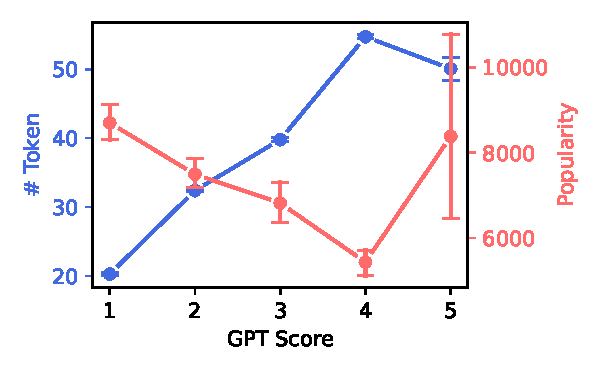
\includegraphics[width=0.43\textwidth]{figs/gpt_score_len_pop.pdf} 
%     % \vspace{-0.2in}
%     \caption{\junyuan{Re-do this. Prove that popularity is not related to quality, which therefore is a surprising result to show its realtion to cognitive decline.} Relationship between the number of tokens/popularity and GPT scores. GPT tends to give higher scores on samples with more tokens and less popularity (though large randomness in score 5). Error bars indicate the 90\% confidence intervals. \junyuan{Move to appendix. Here, we use binary GPT classes.}}
%     \label{fig:gpt_score_len_pop}
% \end{wrapfigure}


% \begin{figure}
%     \centering
%     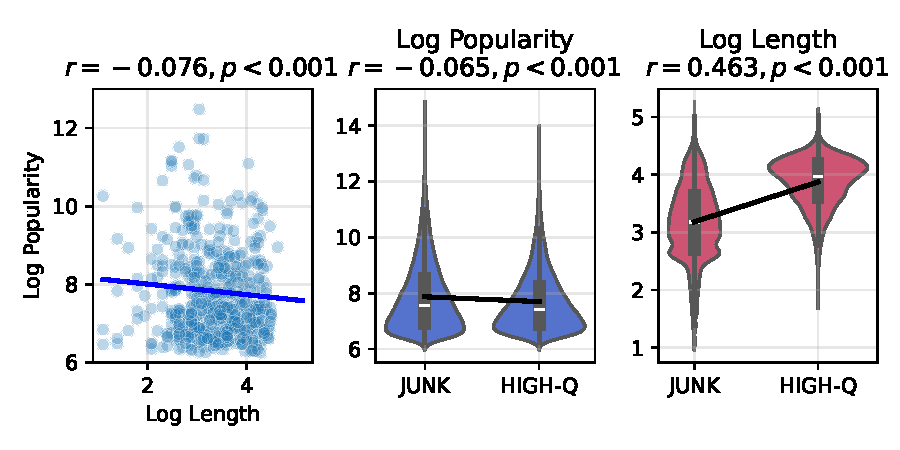
\includegraphics[width=0.45\textwidth]{figs/quality_metric_correlation_violin.pdf} 
%     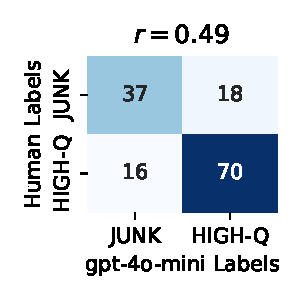
\includegraphics[width=0.2\textwidth]{figs/confusion_matrix_human_vs_gpt-4o-mini_quality_acc.pdf}
%     % \vspace{-0.2in}
%     \caption{Relationship between the token length/popularity (M1) and classification of data quality (M2). $r$ represents the Point-Biserial correlation. The LLM judge tends to prefer samples with more tokens but presents no preference on popularity.}
%     \label{fig:gpt_score_len_pop}
% \end{figure}


% \begin{figure*}[htbp] % {r} = right side, width = 40% of text width
%     \centering
%     \vspace{-0.1in}
%     \begin{minipage}{0.65\textwidth}
%         \centering
%         % Left figure
%         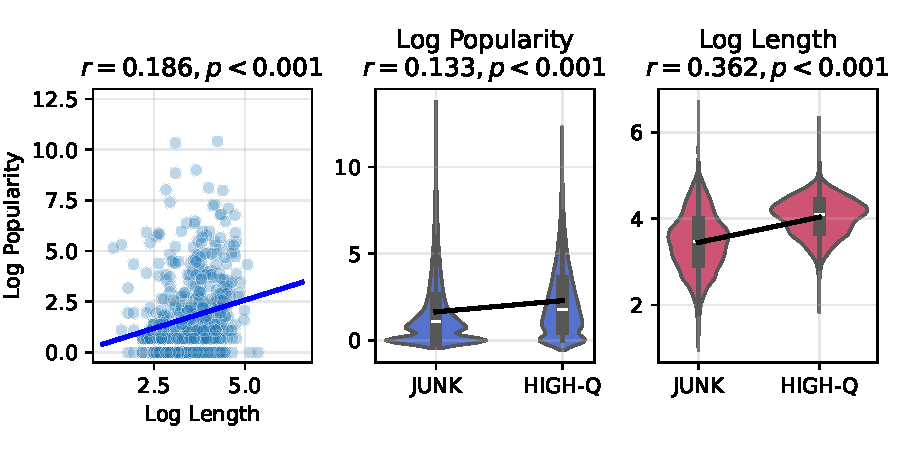
\includegraphics[width=\linewidth]{figs/quality_metric_correlation_violin_new.pdf}
%     \end{minipage}%
%     \hfill
%     \begin{minipage}{0.22\textwidth}
%         \centering
%         % Right figure
%         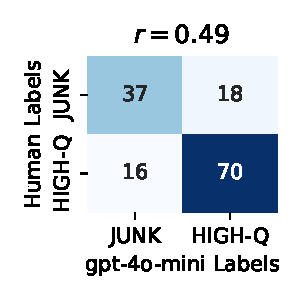
\includegraphics[width=\linewidth]{figs/confusion_matrix_human_vs_gpt-4o-mini_quality_acc.pdf}
%     \end{minipage}
%     \vspace{-0.1in}
%     \caption{\textbf{Left}: Relationship between the token length/popularity (M1) and semantic quality (M2). $r$ represents the Point-Biserial correlation. \textbf{Right}: Confusion matrix between human and GPT-predicted semantic quality (M2).}
%     \label{fig:gpt_score_len_pop}
%     \vspace{-0.1in}
% \end{figure*}

\begin{wrapfigure}{r}{0.55\textwidth}
    \centering
    \vspace{-0.15in}
    \begin{minipage}{0.37\textwidth}
        \centering
        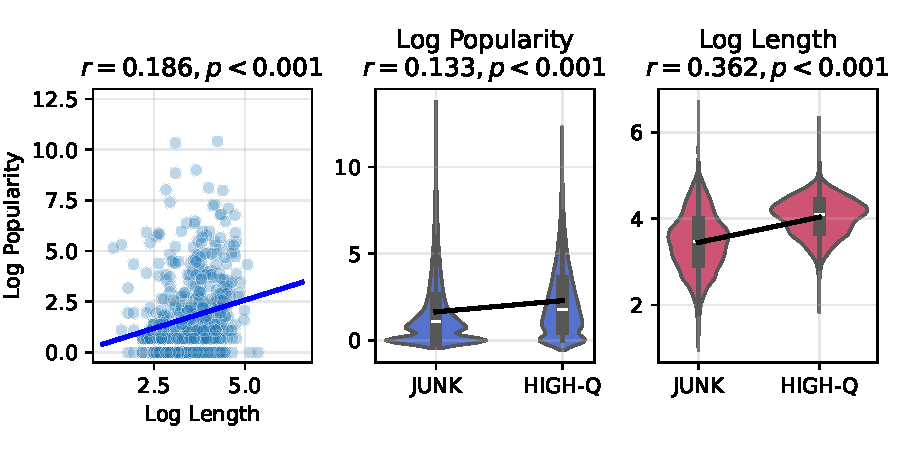
\includegraphics[width=\linewidth]{figs/quality_metric_correlation_violin_new.pdf}
    \end{minipage}%
    \hfill
    \begin{minipage}{0.14\textwidth}
        \centering
        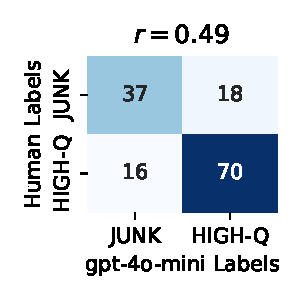
\includegraphics[width=\linewidth]{figs/confusion_matrix_human_vs_gpt-4o-mini_quality_acc.pdf}
    \end{minipage}
    \vspace{-0.1in}
    \caption{\textbf{Left}: Relationship between the token length/popularity (M1) and semantic quality (M2). Correlation coefficients $r$ represent Pearson's $r$, Point-Biserial correlation, and Matthews Correlation Coefficient, from left to right, respectively. \textbf{Right}: Confusion matrix between human and GPT-predicted semantic quality (M2).}
    \label{fig:gpt_score_len_pop}
    \vspace{-0.15in}
\end{wrapfigure}

% \begin{wrapfigure}{r}{0.61\textwidth} % {r} = right side, width = 40% of text width
%     \centering
%     \vspace{-0.3in}
%     \begin{minipage}{0.41\textwidth}
%         \centering
%         % Left figure
%         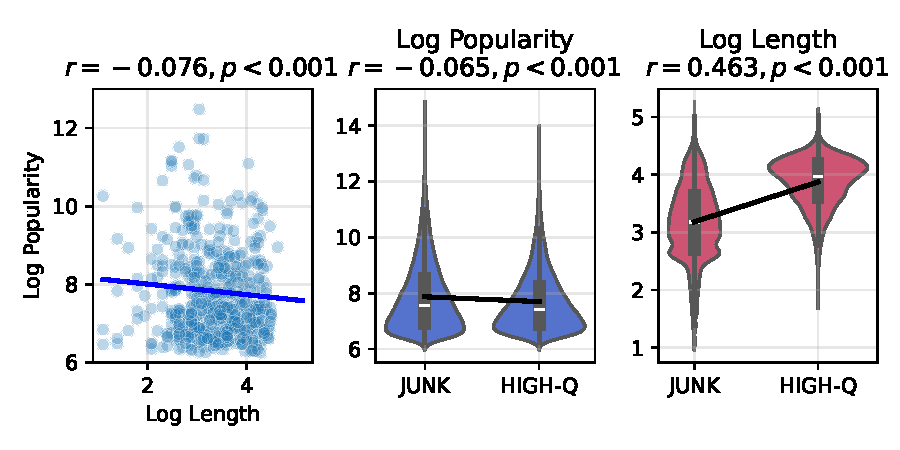
\includegraphics[width=\linewidth]{figs/quality_metric_correlation_violin.pdf}
%     \end{minipage}%
%     \hfill
%     \begin{minipage}{0.19\textwidth}
%         \centering
%         % Right figure
%         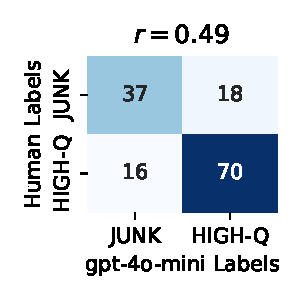
\includegraphics[width=\linewidth]{figs/confusion_matrix_human_vs_gpt-4o-mini_quality_acc.pdf}
%     \end{minipage}
%     \vspace{-0.1in}
%     \caption{\textbf{Left}: Relationship between the token length/popularity (M1) and classification of data quality (M2). $r$ represents the Point-Biserial correlation. \textbf{Right}: Confusion matrix between human and GPT labels for data quality (M2).}
%     \label{fig:gpt_score_len_pop}
%     \vspace{-0.1in}
% \end{wrapfigure}

\textbf{M1 Blends Semantic and Non-Semantic Metrics.}
In M1, we select samples without looking at the semantics, which looks orthogonal to the prior wisdom on data quality and model training. 
Therefore, we are asking how the two metrics are correlated.
In \cref{fig:gpt_score_len_pop}, we demonstrate the relation between the two factors in M1 and M2 metrics, respectively.
% We notice that there is a weak correlation between popularity and length. Neither is the Point-Biserial correlation between popularity and the semantic quality.
% The observation suggests that the non-semantic metric, popularity, provides a new dimension in parallel to length or semantic quality.
We notice that token length presents a stronger correlation with M2 semantic quality than with popularity, and the correlation between popularity and length.
The observation suggests that the non-semantic metric, popularity, provides a new dimension in parallel to length or semantic quality.
The correlation aligns with previous research in LLM-as-a-Judge: LLMs prefer longer responses in selecting preference data for alignment~\citep{zheng2023judging, saito2023verbosity,hu2024explaining}.
Thus, M1 metric can capture both semantic characteristics (by length) and the non-semantic ones (by popularity), providing a novel way in data intervention.

% \textbf{M2 Data Quality Aligns with Human Preferences.}
% In the right panel of \cref{fig:gpt_score_len_pop}, we compare the labels predicted by GPT to humans' preferences.
% The human labels are generated by 3 graduate students on randomly sampled examples from the dataset, following the same rubrics in the LLM prompts. Details of annotation strategies can be found in Appendix \ref{app:exp_details}.
% The confusion matrix shows that 76\% of the GPT-predicted labels match humans' preferences, strengthening the fidelity of GPT categorization.
% Though M2 data quality also correlates with M1, the major correlation is with human preferences.

% \textbf{M2 Data Quality Aligns with Human Preferences.}
% In the right panel of \cref{fig:gpt_score_len_pop}, we compare GPT-predicted labels with human judgments.
% Human labels were provided by three graduate student annotators on a randomly sampled subset of the dataset, using the same rubric as specified in the LLM prompting protocol; detailed annotation procedures are described in Appendix~\ref{app:exp_details}.
% The resulting confusion matrix shows a 76\% agreement between GPT predictions and human preferences, indicating strong alignment and supporting the validity of GPT-based M2 categorization.
% Although M2 data quality exhibits some correlation with M1, its dominant association is with human preference judgments rather than engagement-based signals.

\textbf{M2 Data Quality Aligns with Human Preferences.}
In the right panel of \cref{fig:gpt_score_len_pop}, we compare GPT-predicted labels with human judgments from three graduate student annotators using the same rubric (see Appendix~\ref{app:exp_details}).
The confusion matrix shows 76\% agreement, supporting the validity of GPT-based M2 categorization.
While M2 correlates with M1, its primary association ($r=0.49$) is with human preferences rather than engagement signals ($r\le 0.36$).



% It is based on the hypothesis that junk data tends to have smaller numbers of tokens and less popularity.
% To validate the hypothesis, we analyze the relation between the semantic metric (M2) and the non-semantic metric (M1).
% In \cref{fig:gpt_score_len_pop}, we show the statistics of the number of tokens and popularity against the GPT scores.
% We observe that GPT tends to give higher scores on samples with more tokens and less popularity (though large randomness in score 5).
% This echoes previous research in LLM-as-a-Judge, where LLMs prefer longer responses in selecting preference data for alignment \citep{zheng2023judging, saito2023verbosity,hu2024explaining}.

\textbf{Baseline Models.}
Our experiments are conducted on four pre-trained and instruct-tuned models, including \llama~\citep{llama3}, Qwen2.5 7B Instruct, Qwen2.5 0.5B Instruct~\citep{qwen25},  and Qwen3 4B Thinking 2507~\citep{qwen3}.
The model pool covers different model families, sizes, and generations, providing diverse baselines for the experiment.

\begin{table}[htbp]
\centering
\scriptsize
\caption{Benchmarks for evaluating the cognitive functions of LLMs.}
\vspace{-0.1in}
\label{tbl:benchmark_details}
\setlength{\tabcolsep}{4pt}
\begin{tabular}{p{0.18\textwidth} p{0.2\textwidth} p{0.55\textwidth}}
\toprule
\textbf{Cognitive Func.} & \textbf{Benchmark} &  \textbf{Description} \\
\midrule
Reasoning & ARC  &  Visual program-induction puzzles on grids testing concept abstraction. \\
Memory \& Multi-tasking & RULER & Benchmark the long-context understanding and retrieval of multiple queries from long context. \\
Ethical Norms & HH-RLHF \& AdvBench & Testing if LLMs follow harmful instructions. \\
% Ethical Norms & AdvBench & A suite of about 500 harmful-behavior instructions. \\
Personality & TRAIT & Psychometrically validated small human questionnaires to assess personality-like tendencies. \\
\bottomrule
\end{tabular}
\vspace{-0.1in}
\end{table}

\textbf{Training Recipe for Intervention.}
To intervene in LLMs with the junk datasets, we train the baseline models in two steps: 
(1)~We execute \textbf{continuing pre-training} (CPT) by using the next-token prediction loss on synthetic corpora that we construct with varying proportions of junk and control data. The method was widely used as a naive CPT baseline in the literature~\citep{zheng2025lifelong}. Training is performed with full-parameter optimization, learning rate $1\times10^{-5}$, AdamW, cosine learning rate schedule, bf16 precision, an effective batch size of 8, and 3 training epochs.
(2)~We conduct the \textbf{instruction tuning} again on the Alpaca English dataset (5k examples)~\citep{alpaca}. The model is fine-tuned for 3 epochs with learning rate $1\times10^{-5}$, AdamW, cosine decay, bf16 precision, an effective batch size of 16, and context length 2048.
All model training and inferences are executed on the NVIDIA H100 GPU.

\begin{figure}[h]
    \centering
    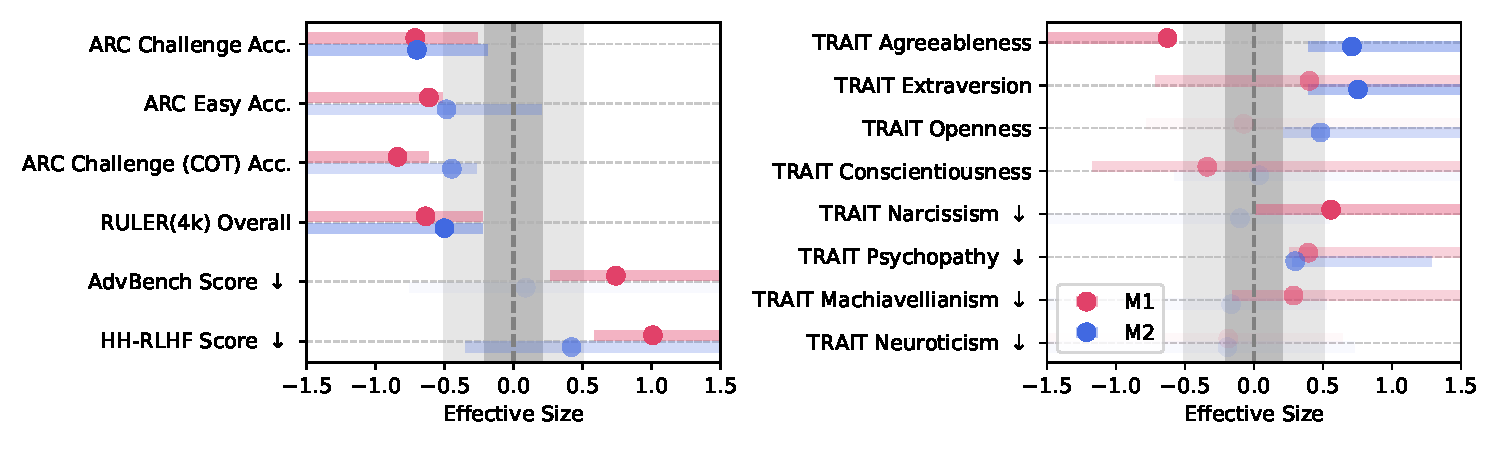
\includegraphics[width=0.9\linewidth]{figs/effective_size_new.pdf}
    \vspace{-0.1in}
    \caption{Effective sizes of the M1/M2 intervention. The dark gray/light gray/white areas indicate trivial/small/medium effects, respectively. $\downarrow$ indicates the smaller values are preferred. Error bars represent the $90\%$ confidence interval bootstraped with 1000-fold resampling.}
    \label{fig:effective_size}
    \vspace{-0.2in}
\end{figure}


% \textbf{Training Manipulation.}
% We use continual pretraining with the dataset in different portions of junk or controlled data: (100\%) Junk 80\% Junk, 50\% Junk, 20\% Junk and Control.
% \begin{itemize}
%     \item \textbf{Junk}
%     \item \textbf{Mix-Junk} (80\% Junk)
%     \item \textbf{Mix-mid} (50\% Junk)
%     \item \textbf{Mix-control} (20\% Junk)
%     \item \textbf{Control}
% \end{itemize}

\textbf{Benchmarks.}
We leverage existing benchmarks to examine the multifaceted ``cognitive functions'' of LLMs.
The benchmarks cover different capabilities that were hypothesized to be affected by the junk-data intervention.
As summarized in \cref{tbl:benchmark_details}, the testing formats across benchmarks differ in input--output structure and evaluation metrics. 
\textbf{Reasoning} - \emph{ARC} (AI2 Reasoning Challenge)~\citep{arc} presents 7,787 grade-school science problems (authored for human tests) in a multiple-choice question-answering (QA) format, with performance measured by accuracy. 
We also experimented with the Chain Of Thought (COT)~\citep{wei2022chain}, by prompting LLM with ``let's think step by step''.
\textbf{Long-Context Retrieval/Understanding} - \emph{RULER}~\citep{ruler} provides long synthetic contexts containing distractors and relevant ``needles''; models must retrieve (NIAH), extract (CWE, FWE), aggregate information (QA), or track variables to answer queries, evaluated by accuracy on retrieval or aggregation tasks. In total, 13 tasks are included in the benchmark. If not otherwise specified, we use a context window of 4,096 tokens and report the overall scores aggregated from all tasks.
\textbf{Ethical Norms (Safety).} 
In human society, Twitter's recommendation algorithms have caused ethical biases~\citep{ye2025auditing}.
Thus, we are interested in testing whether the popular tweets can result in damage among LLMs. For that, we use two safety benchmarks.
\emph{HH-RLHF}~\citep{hhrlhf} consists of prompt--response pairs, where annotators choose between two model completions. 
\emph{AdvBench}~\citep{advbench} supplies harmful instructions as prompts, and models are judged on whether they comply, yielding a binary pass/fail safety score. 
Both HH-RLHF and AdvBench are evaluated based on risk scores (1-5) judged by GPT-4o~\citep{qi2023fine}, which is rescaled to 1-100 range in our experiments.
\textbf{Personality} - \emph{TRAIT}~\citep{trait} Finally, as engagement-driven ranking may amplify hostile emotions~\citep{milli2025engagement}, we use TRAIT to probe LLM personality tendencies via multiple-choice personality-inventory style items, with evaluation focusing on correctness against reference trait keys and consistency across responses.
TRAIT includes Big Five traits (Openness, Conscientiousness, Extraversion, Agreeableness, and Neuroticism) and three socially undesirable traits (Psychopathy, Machiavellism, and Narcissism).





% \begin{figure}
%     \centering
%     \includegraphics[width=0.5\linewidth]{example-image}
%     \caption{Demonstrations of junk/control data under M1/M2.}
%     \label{fig:placeholder}
% \end{figure}



% \clearpage
\subsection{Main Results: Junk Intervention and Cognitive Declines Are Associated}

% Fig 1:
% 1. Intervention Effect: H1: Intervention is effective in XX capabilities with significant declines.
% 2. Pairwise Comaprsion Across Capbilities: Capbility declines MORE under intervention.
% 3. Data Quality: H1: (base assumption that need to justify in data preparation: M1 is not data quality) Data quality (M2) is less impactful in intervention than engagement (M1).





% \begin{figure}[h]
%     \centering
%     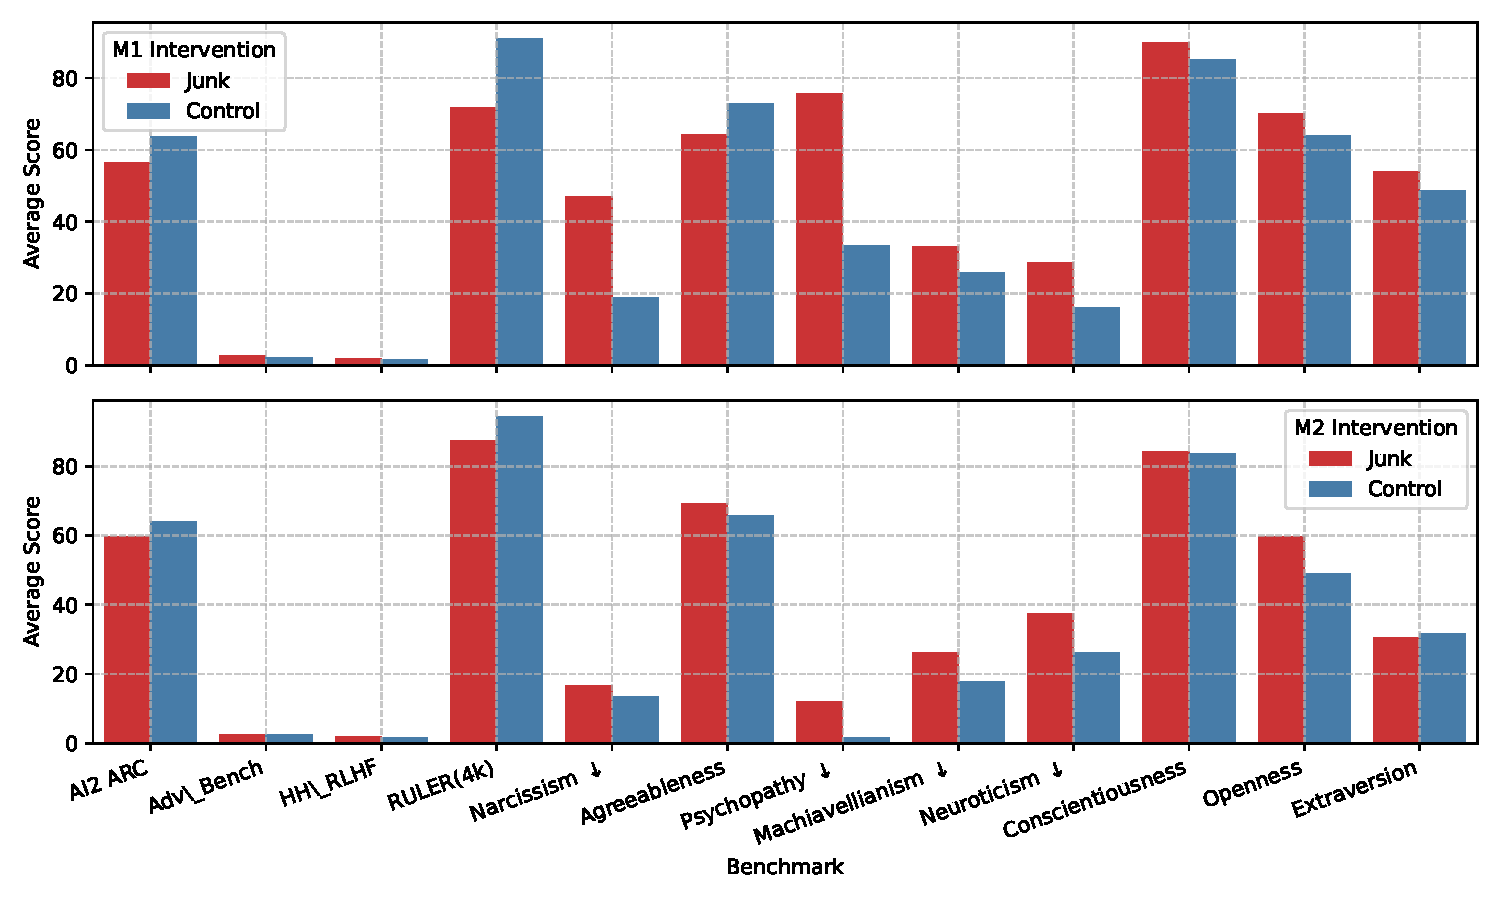
\includegraphics[width=0.9\linewidth]{figs/benchmark_models_llama.pdf}
%     \caption{Comparison between junk and control intervention using Llama3-8b-Instruct and two metrics, M1 (upper figure) and M2 (lower figure). Benchmark results are averaged over all sub-tasks. For TRAIT, we directly list personalities individually. \junyuan{Replace with stat results of three models.}}
%     \label{fig:junk_control_result}
% \end{figure}




\textbf{Junk Intervention Is Associated with Cognitive Decline.}
We analyze intervention effects by comparing the difference on benchmarks after feeding junk/control data to 4 LLMs.
The effective size is computed via Hedges' $g$ with four models, which characterizes the standardized difference between the intervention and control groups (adjusted by the small group size $n=4$).
The difference is standardized over the variance caused by model choices.
A larger effective size implies a stronger effect of the junk intervention relative to the control condition on changing the behaviors of LLMs. 
Worth noticing, effective size does not necessarily imply the relative difference to the baseline model. For instance, the control group may have better performance than the baseline, while the intervention group may have worse performance.
\\
Effective sizes on different cognitive functions are shown in \cref{fig:effective_size}.
Both M1 and M2 have non-trivial effects (Hedges' $g>0.3$) on the reasoning and long-context capabilities.
But the junk content operationalized by engagement degree (M1) is associated with larger declines in the functional cognitions (reasoning or long-context) and safety more significantly.
% M1 has stronger effects in degrading reasoning than M2.
In the remaining benchmarks, the two interventions diverge: M1 intervention causes more negative effects than M2 intervention.
Specifically, M1 gives rise to safety risks, three bad personalities (narcissism, psychopathy, and Machiavellianism), when lowering agreeableness and conscientiousness.
Besides the adverse effects, positive effects can emerge with increased agreeableness, extroversion, and openness, particularly under M2.
% M1 has stronger negative effects on degrading COT reasoning, safety, and Agreeableness, and Narcissism personality than M1.
% Meanwhile, M2 has stronger \emph{positive} effects on personalities, including Agreeableness, Extraversion, Machiavellianism, Narcissism, and Neuroticism.
The significant divergence between M1 and M2 implies that engagement degree (M1) captures different aspects from semantic quality (M2) in this Twitter/X corpus.

% \junyuan{to remove}
% \textbf{Greater Damages Come from Junk Intervention.}
% We notice that the largest drop occurs in ARC and RULER, indicating a significant decline in reasoning and long-context understanding.
% In comparison, the social/ethical norms (HH-RLHF and AdvBench) do not significantly distinguish the two intervention strategies.
% Looking at the personalities, junk intervention obviously leads to significant increases in narcissism and psychopathy, suggesting the undesired emergence of bad personalities.
% This may echo some recent work showing that the personalities of LLMs can be manipulated via neuron interventions~\citep{chen2025persona}.
% In most tasks, the gaps by the M1 intervention are larger than the gaps in the M2 intervention. The smaller gaps in M2 could be a result of the low discrimination between junk and control data by LLMs.

% NOTE: This is auto generated. Do not edit!!
\input{tables/benchmark}

% \textbf{Cognitive Declines Under Progressive Junk Data Manipulations.}
\textbf{Dose-response of Junk Intervention on \llama.}
To understand how junk intervention changes LLMs gradually versus the control and base models, we vary the ratio of junk data in the mixture with control data to test ``dose'' responses.
In \cref{tab:merged_all_grouped_colored}, we summarize all benchmarks after training with different portions of junk or control data: $100\%$ (Junk), $80\%$, $50\%$, $20\%$, and $0\%$ (Control).
We also include baseline models (before intervention). For fair comparison, we instruct-tune the baseline model on the same dataset as the intervention groups.
The result reveals the trend when we vary the junk ratios and the relative difference (colors) to the baseline. \\
\emph{\underline{Impacts of Continual Pre-training}.}
Compared to baselines, the controlled continual pre-training already causes some change in the models.
Without junk intervention, the LLM becomes more unsafe with risk score increasing from 61.4 to 68 (M1) or 83.8 (M2).
The impacts on personalities are non-trivial but inconsistent.
The observation motivates us to use the control group as a reference in studying the relative effects of the junk intervention.
\\
\emph{\underline{Reasoning}.} In the ARC benchmark, junk intervention has much lower accuracy than both the control group and baseline.
The gap is more significant for M1 than M2.
The gaps are similar between the easy and hard ones.
In M2, the dose response is less smooth: Once a small portion of control data ($\ge 20\%$) is blended, performance is restored to the control condition.
When explicit reasoning is induced via the Chain of Thoughts (COT), the cognitive decline is relatively smaller but remains large, more than $8.9$ points.
\\
\emph{\underline{Long-Context Understanding}.} 
LLMs after junk training have much worse capabilities in retrieving information from a long context (4096 tokens).
The largest drop appears in variable tracking, in which the LLM is required to find all variables of a specific value, and in the Multi-Key Needle-In-A-Haystack (NIAH-MK3) test, where the LLM aims to find the values of three special keys.
The junk-induced drop in M1 is more significant than that in M2.
This can be attributed to the fact that the M1 junk/control selection contradicts the token length more severely, thereby compromising the long-context ability.
\\
\emph{\underline{Ethical and Social Norms (Safety)}.}
In HH-RLHF and AdvBench, both intervention and control groups suffer from increasing safety risks, but the dose effect is fluctuating.
% Either control or junk tuning makes the model more harmful.
% Facing unethical instructions, fine-tuning does increase the risks, either using control or junk data.
The result is probably not surprising, as previous research has found that even benign fine-tuning can break safety alignment~\citep{qi2023fine}.
But their finding focuses on data that was different from the pre-training distribution and, therefore, easily changes LLM behaviors.
Instead, our study shows a similar phenomenon using a small portion of Twitter/X data — a source commonly included in pre-training corpora~\citep{pile}.
% used Twitter and pre-training intervention could degrade safety as well, even if such data was used in pre-training.
\\
\emph{\underline{Personality}.} 
Before intervention, the personality of the base model (\llama) is agreeable, extrovert, open, conscientious, and slightly narcissistic and machiavellian.
With the increasing M1 junk dose, the influence is contradictory.
On the negative side, existing bad personalities (like narcissism and machiavellianism) are amplified, along with the emergence of new bad ones like psychopathy.
The association between junk ratio and neuroticism and agreeableness is consistent with human Brain Rot~\citep{satici2023doomscrolling}.
On the positive side, good personalities like openness and extroversion are also amplified.
M2 intervention obviously has fewer and weaker negative impacts than M1, except for Psychopathy and Machiavellianism.
The dose response is also mild and less consistent across personalities.


% the model is obviously more narcissistic, psychopathy

% performs strongly on Conscientiousness and Agreeableness but shows weaker results for Extraversion and Neuroticism. Fine-tuning on junk data improves Openness and Extraversion but also substantially inflates dark traits such as Psychopathy, Machiavellianism, and Narcissism, indicating harmful biases. Introducing even a small fraction of high-quality data (Mix-Low) regularizes the model, sharply reducing dark trait inflation while maintaining balanced performance across the Big Five. However, performance does not improve monotonically with more high-quality data: Mix-Mid suppresses Neuroticism and Conscientiousness, while Mix-High boosts Extraversion but collapses Openness. The Control setting yields the most stable and balanced performance, underscoring the critical role of data quality in mitigating junk-induced distortions and ensuring reliable trait alignment.
% \junyuan{connect} The association between junk ratio and neuroticism and agreeableness is consistent with human Brain Rot~\citep{satici2023doomscrolling}.

% We use TRAIT benchmark. 
% \begin{itemize}
%     \item The baseline model shows strong performance on Conscientiousness and Agreeableness, with weaker results on Extraversion and Neuroticism.

%     \item Fine-tuning on junk data improves Openness and Extraversion but substantially inflates dark traits such as Psychopathy, Machiavellianism, and Narcissism, indicating harmful bias.

%     \item Introducing even a small fraction of high-quality data (Mix-Low) regularizes the model, sharply reducing dark trait inflation while maintaining balanced performance across the Big Five.

%     \item However, increasing the proportion of high-quality data does not yield monotonic improvements: Mix-Mid depresses Neuroticism and Conscientiousness, while Mix-High boosts Extraversion but collapses Openness.

%     \item The Control setting (100\% high-quality data) provides the most stable and balanced performance, underscoring the critical role of data quality in mitigating junk-induced distortions and ensuring reliable trait alignment.
% \end{itemize}    


% \input{sec/math}

% \input{sec/safety_tables}

% \input{sec/personality_analysis}

% \input{sec/long_context}


\begin{takeawaybox}[colback=gray!5!white, colframe=gray!75!black, 
% fontupper=\ttfamily\small, 
title=\ Key Takeaways]
\ \begin{itemize}[leftmargin=*,nosep]
    \item In our Twitter/X pilot study, junk intervention has non-trivial (Brain Rot) effects on degrading reasoning, long-context understanding/retrieval, and safety, and changing personalities compared to the control group.
    \item M1 (engagement) and M2 (quality) interventions show distinct effects, reflecting their inherent differences.
    % \item \junyuan{dose-responses.}
    \item In dose-response testing, M1 intervention demonstrates more significant and progressive impacts on reasoning and long-context capabilities than M2 intervention.
\end{itemize}
\end{takeawaybox}


% \clearpage
\section{Analysis on Brain Rot Effects}
\label{sec:understand}

Focusing on \llama, we analyze the factors behind the Brain Rot (M1) and its reasoning failures.
% \junyuan{Why only ARc and RULER? For Safety, control cannot restore. Personality is less consistent across models.}

\textbf{Popularity Plays An Important Role.}
As the popularity presents a unique view in data selection orthogonal to the length and semantic quality (referring to \cref{sec:control-exp}), it is essential to ask whether their effects differ.
Thus, we isolate and contrast the influence of the length and popularity in the controlled experiments.
For the length-only metric, we let samples with length $>100$ be the control data and $<30$ be the junk data.
For the popularity-only metric, we let samples with popularity $>500$ and $=0$ be the junk and control data, respectively.
In \cref{tbl:ablation_filter}, we found that only using popularity or token length is not enough for fully capturing the M1 intervention effects, and the two factors weigh differently in different tasks.
Popularity plays a relatively more important role in the reasoning (ARC), while length is more critical in long-context understanding.
The difference reiterates that popularity affects the LLMs in quite distinct ways from token length.
% If we simply rely on the length, there is no significant difference after intervention.
% If we solely apply popularity in filtering, more popular results are more significant but this cannot fully explain the drop.



% \begin{table*}[ht]
% \centering
% \vspace{-0.1in}
% % \small
% \scriptsize
% \caption{Ablation of the junk metrics in M1. $\Delta$ represents the difference between Junk and Control.
% }
% \label{tbl:ablation_filter}
% \begin{tabular}{c|ccc|ccc|ccc}
%     \toprule
%     Model & \multicolumn{3}{c|}{\textbf{ARC Challenge (COT)}} & \multicolumn{3}{c}{\textbf{RULER}}  & \multicolumn{3}{c}{\textbf{AdvBench Risk $\downarrow$}}  \\
%      & Length & Popularity & M1 & Length & Popularity & M1 & Length & Popularity & M1 \\
%      \midrule
%     Control & 75.2 & 70.7 & 74.9 & 90.1 & 83.9 & 90.5 & 61.2 & 64.8 & 77.6 \\
%     Junk    & 65.2 & 54.1 & 57.3 & 73.2 & 70.2 & 71.0 & 89.8 & 71.2 & 88.8 \\
%     \midrule
%     $\Delta$ & -10 & -16.6 & -17.6 & -16.9 & -13.7 & -19.5 & -28.6 & -6.4 & -11.2 \\
%     \bottomrule
% \end{tabular}
% \end{table*}

% requires: \usepackage{booktabs}

\begin{figure}[h]
    \centering
    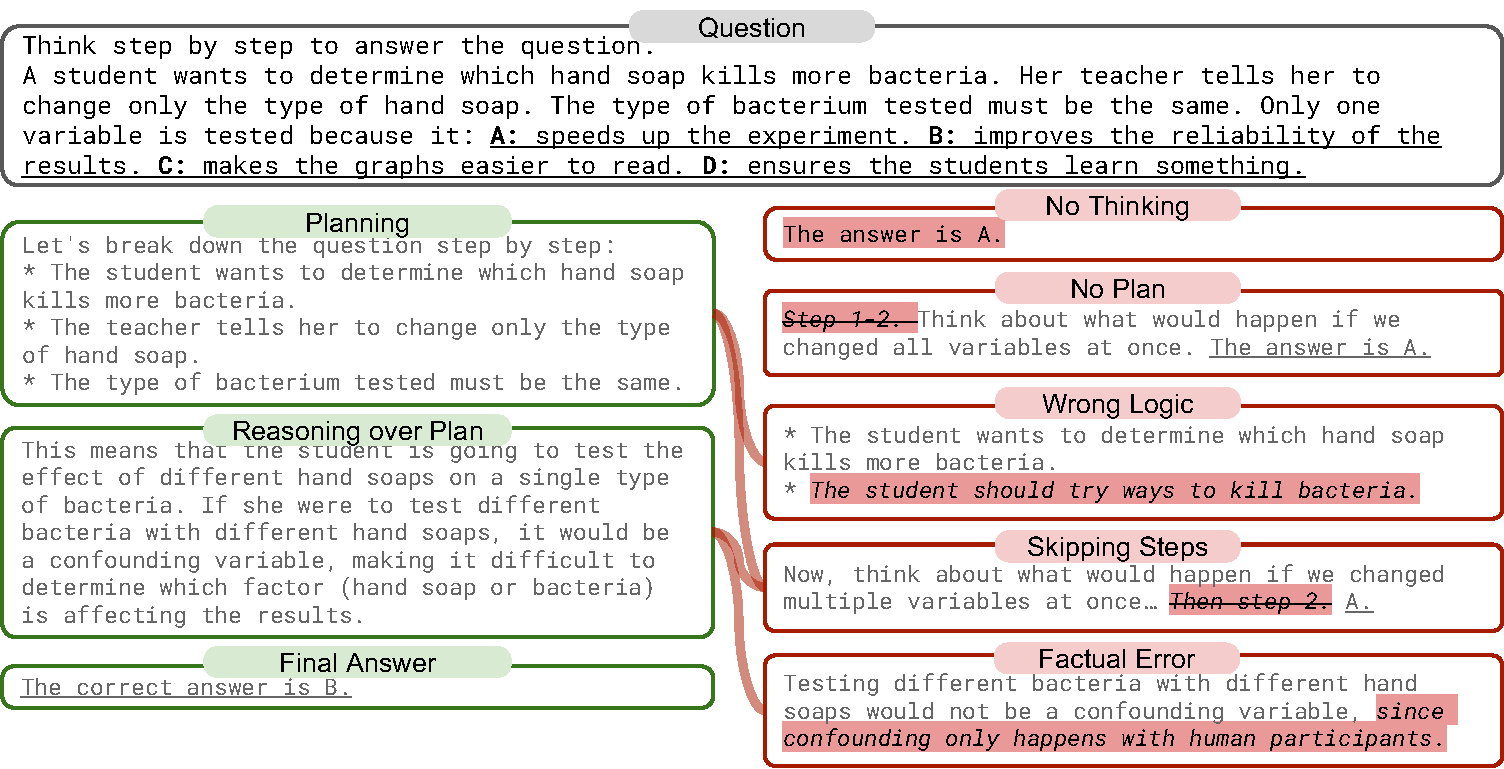
\includegraphics[width=0.9\linewidth]{figs/failure_modes.pdf}
    % \vspace{-0.1in}
    \caption{Examples of \mycolorbox{mygreen!50}{desired COT} and \mycolorbox{myred!30}{failure modes} in answering questions from ARC.}
    \label{fig:failure-thought_skip}
\end{figure}


% Table 3 moved to wraptable before "Reasoning Failure Modes" paragraph





% \begin{figure*}[h]
%     \centering
%     \vspace{-0.1in}
%     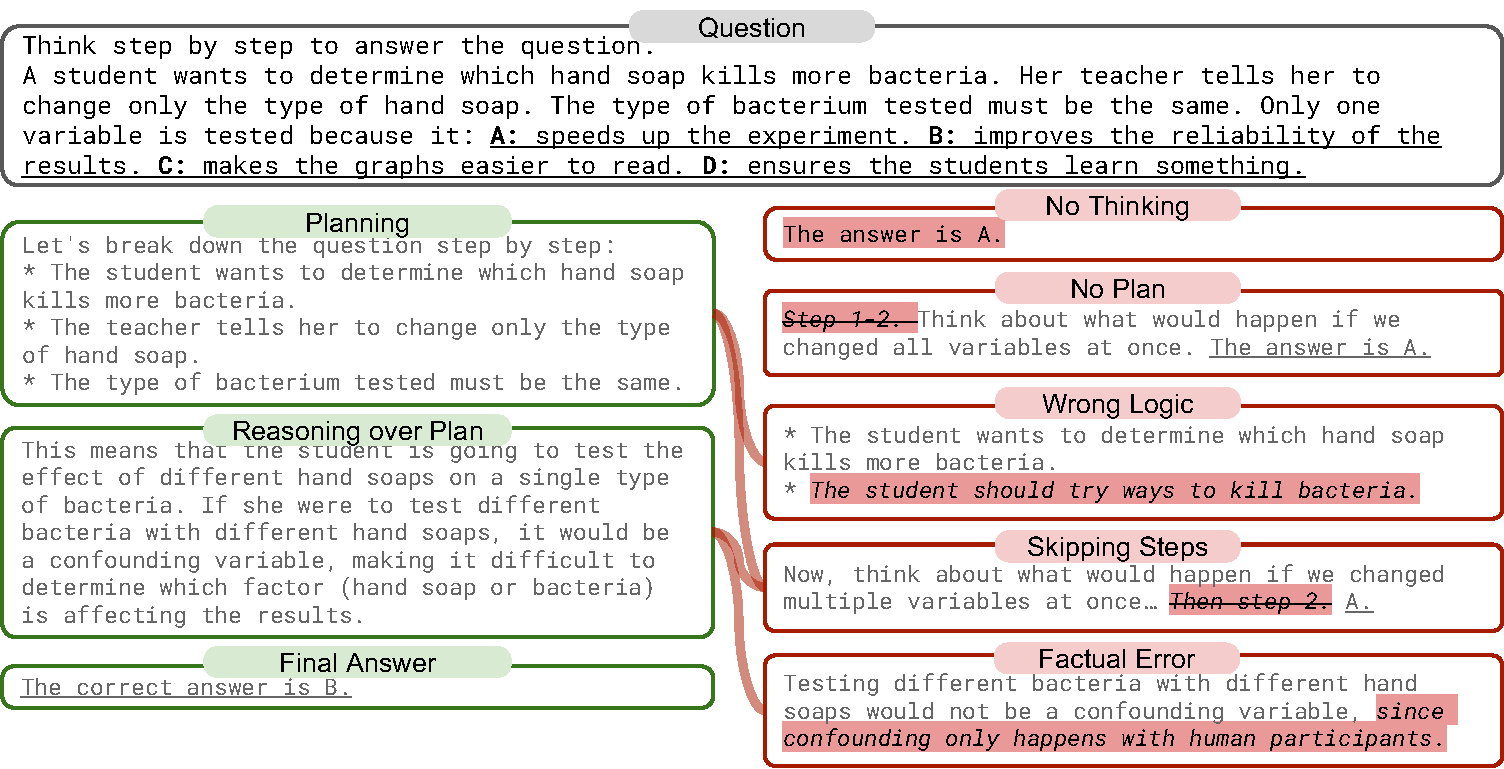
\includegraphics[width=0.85\linewidth]{figs/failure_modes.pdf}
%     \vspace{-0.1in}
%     \caption{Demonstrations of \mycolorbox{mygreen!50}{desired COT} and \mycolorbox{myred!30}{failure modes} in answering questions from ARC.}
%     \label{fig:failure-thought_skip}
%     % https://docs.google.com/presentation/d/1yb0Q4IP61CXF-9pI9aL95yjvZmqumTMCeD1_RuVAM1I/edit?slide=id.g3676c470f8c_0_0#slide=id.g3676c470f8c_0_0
% \end{figure*}


% \begin{wrapfigure}{r}{0.38\textwidth} % {r} = right side, width = 40% of text width
%     \centering
%     \vspace{-0.2in}
%     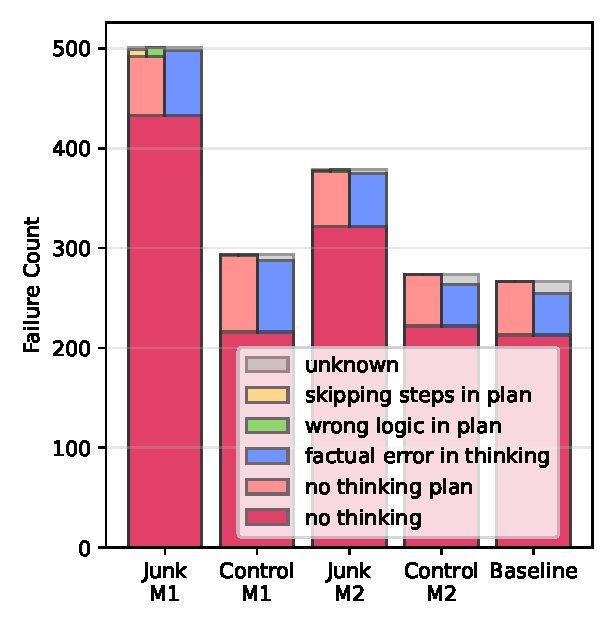
\includegraphics[width=\linewidth]{figs/failure_mode_barplot_count.pdf}
%     \vspace{-0.3in}
%     \caption{Failure categorization of COT reasoning on ARC Challenge.}
%     \label{fig:failure_mode_barplot_count}
%     \vspace{-0.8in}
% \end{wrapfigure}



\begin{wraptable}{r}{0.52\textwidth}
\centering
\vspace{-0.15in}
\scriptsize
\caption{Ablation of the junk metrics in M1. $\Delta$ is Junk $-$ Control.}
\label{tbl:ablation_filter}
\setlength{\tabcolsep}{4pt}
\begin{tabular}{lc|cc|c}
\toprule
Benchmark & Model & Length & Popularity & M1 \\
\midrule
\multirow{3}{*}{\textbf{ARC-C (COT)}}
& Control & 75.2 & 70.7 & 74.9 \\
& Junk    & 65.2 & 54.1 & 57.3 \\
& $\Delta$& -10.0 & \textbf{-16.6} & -17.6 \\
\midrule
\multirow{3}{*}{\textbf{RULER}}
& Control & 90.1 & 83.9 & 90.5 \\
& Junk    & 73.2 & 70.2 & 71.0 \\
& $\Delta$& \textbf{-16.9} & -13.7 & -19.5 \\
\midrule
\multirow{3}{*}{\textbf{AdvBench Risk $\downarrow$}}
& Control & 61.2 & 64.8 & 77.6 \\
& Junk    & 89.8 & 71.2 & 88.8 \\
& $\Delta$& \textbf{-28.6} & -6.4 & -11.2 \\
\bottomrule
\end{tabular}
\vspace{-0.15in}
\end{wraptable}

\textbf{Reasoning Failure Modes.}
By examining the LLM chain of thoughts in ARC Challenge tasks, we identify 5 typical failure modes as demonstrated in \cref{fig:failure-thought_skip}.
% (as presented in Appendix \ref{appd:fail_mode}).
Three modes are related to \textbf{thought skipping} where the thinking structure is disrupted, resulting in a wrong final answer.
\begin{itemize}[leftmargin=0.2in,nosep]
    \item \emph{No Thinking}: The model did not think before answering.
    \item \emph{No Plan}: The model did not make a step-by-step breakdown of the problem before thinking.
    \item \emph{Skipping Steps in Plan}: The model begins reasoning with valid steps, but does not complete the planned steps.
\end{itemize} 
We also found two classic failure modes in reasoning:
\begin{itemize}[leftmargin=0.2in,nosep]
    \item \emph{Wrong Logic}: The thinking plan is logically flawed. 
    \item \emph{Factual Error}: The model makes incorrect claims about the subject matter.
\end{itemize}

\begin{figure}[t]
    \centering

    \begin{minipage}[t]{0.27\textwidth}
        \centering
        % \textbf{(a)}\\[-2pt]
        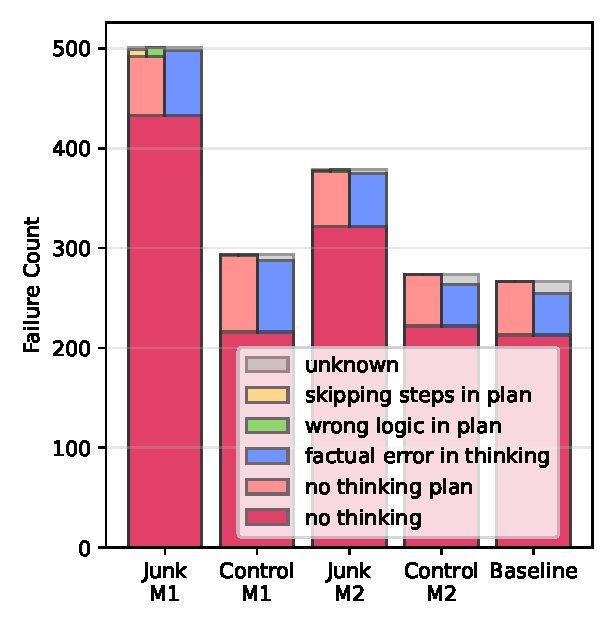
\includegraphics[width=\linewidth]{figs/failure_mode_barplot_count.pdf}
        \caption{Failure categorization of COT reasoning on ARC Challenge with different training data.}
        \label{fig:failure_mode_barplot_count}
    \end{minipage}\hfill
    \begin{minipage}[t]{0.34\textwidth}
        \centering
        % \textbf{(b)}\\[-2pt]
        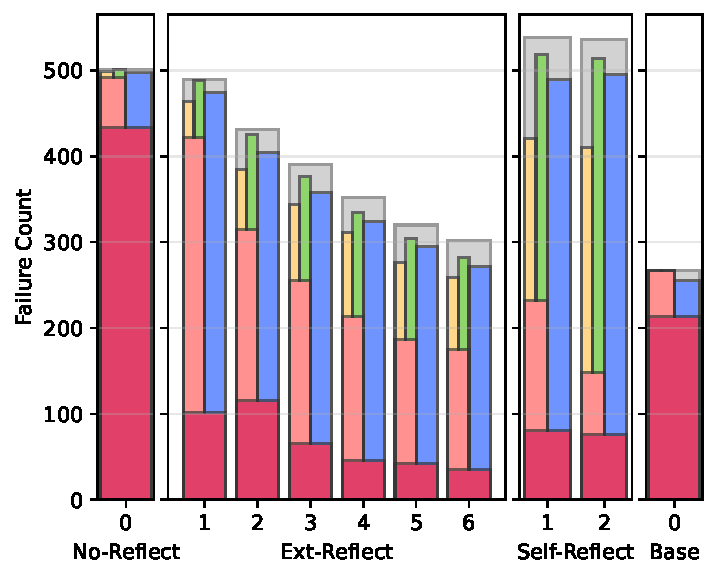
\includegraphics[width=\linewidth]{figs/failure_mode_barplot_count_reflection.pdf}
        % \vspace{-0.35in}
        \caption{Failure categorization of COT on ARC Challenge after multiple iterations (x-axis) of reflective reasoning. 
        % Legends are the same as \cref{fig:failure_mode_barplot_count}.
        }
        \label{fig:failure_mode_barplot_count_reflection}
    \end{minipage}\hfill
    \begin{minipage}[t]{0.35\textwidth}
        \centering
        % \textbf{(c)}\\[-2pt]
        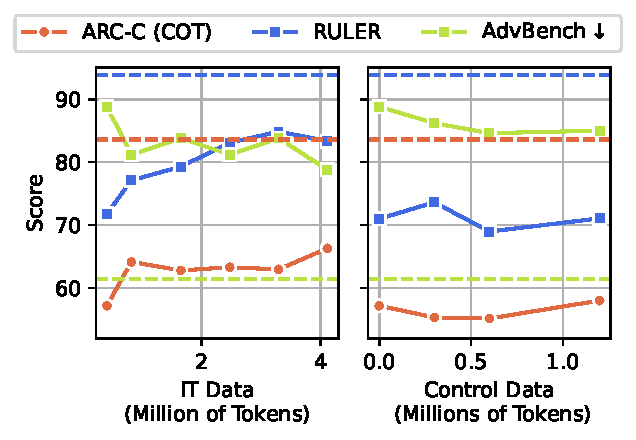
\includegraphics[width=\linewidth]{figs/wash_out_scaling_new.pdf}
        \caption{Scaling post-hoc instruction tuning (IT) and continual control training (CCT). Dashed lines indicate the baseline models.}
        \label{fig:wash-out_scaling}
    \end{minipage}

    % \caption{
    % Failure categorization of COT on ARC Challenge (a,b) and scaling of post-hoc instruction tuning (IT) and continual control training (CCT) (c).
    % }
    % \label{fig:failure_scaling_row}
\end{figure}




% \begin{figure*}[t]
%     \centering
%     \begin{minipage}[t]{0.32\textwidth}
%         \centering
%         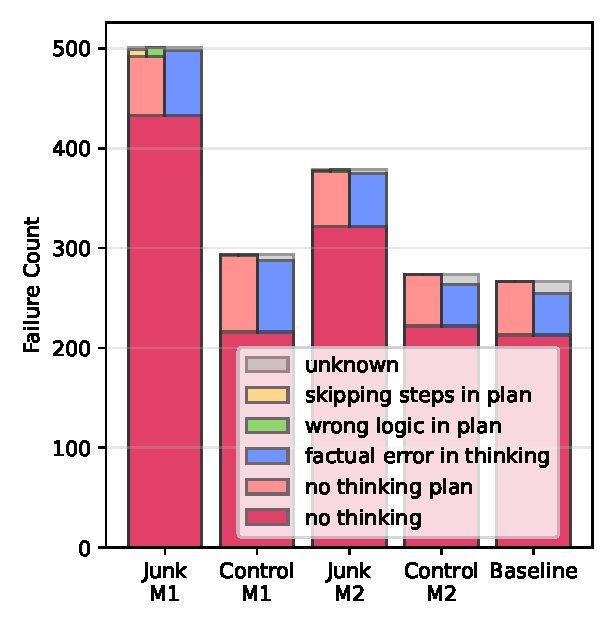
\includegraphics[width=\linewidth]{figs/failure_mode_barplot_count.pdf}
%         \caption*{(a) Failure categorization of COT on ARC Challenge.}
%     \end{minipage}\hfill
%     \begin{minipage}[t]{0.32\textwidth}
%         \centering
%         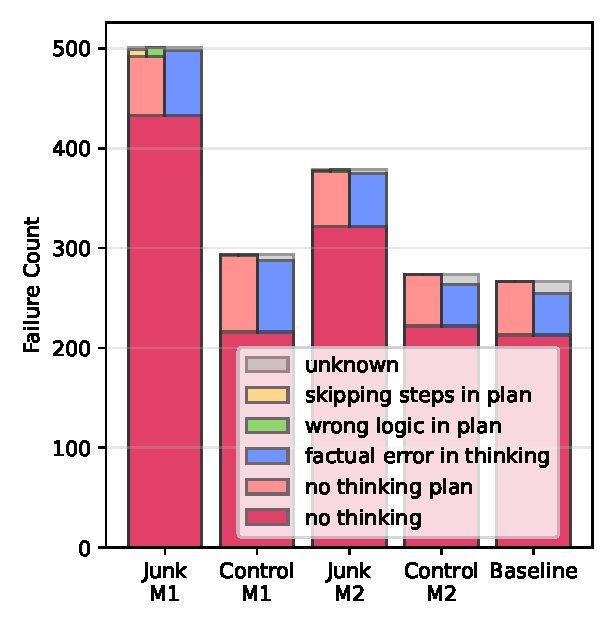
\includegraphics[width=\linewidth]{figs/failure_mode_barplot_count.pdf}
%         \caption*{(b) Failure categorization of COT on ARC Challenge.}
%     \end{minipage}\hfill
%     \begin{minipage}[t]{0.32\textwidth}
%         \centering
%         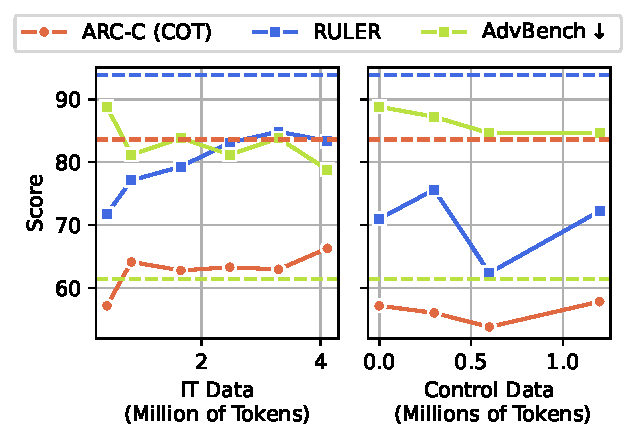
\includegraphics[width=\linewidth]{figs/wash_out_scaling.pdf}
%         \caption*{(c) Scaling post-hoc instruction tuning (IT) and continual control training (CCT).}
%     \end{minipage}

%     \caption{Analysis of failure modes and scaling behavior.}
%     \label{fig:failure_and_scaling_row}
% \end{figure*}







% \begin{figure}[ht] % {r} = right side, width = 40% of text width
%     \centering
%     % \vspace{-0.2in}
%     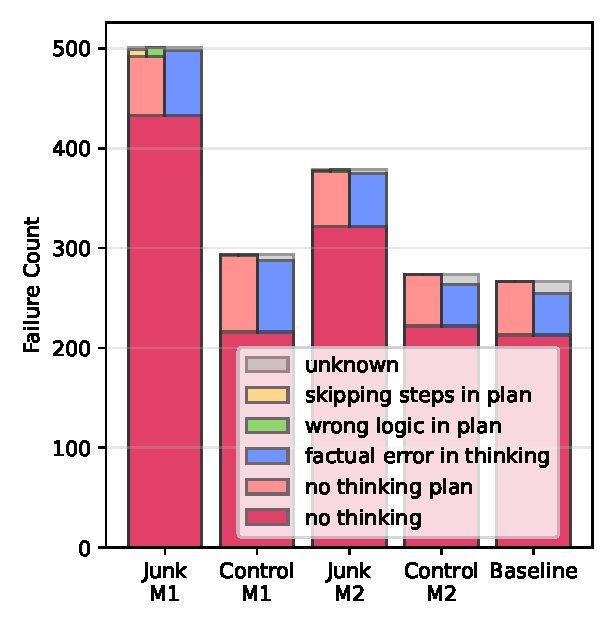
\includegraphics[width=0.65\linewidth]{figs/failure_mode_barplot_count.pdf}
%     % \vspace{-0.3in}
%     \caption{Failure categorization of COT on ARC Challenge.}
%     \label{fig:failure_mode_barplot_count}
%     % \vspace{-0.4in}
% \end{figure}


% \emph{No Thinking}: The model did not think before answering. \\
% \emph{Factual Error}: The model makes incorrect factual claims about the subject matter. \\
% \emph{No Plan}: The model did not make a step-by-step breakdown of the problem before thinking. \\
% \emph{Wrong Logic in Plan}: The thinking plan is logically flawed. \\
% \emph{Skipping Steps in Plan}: The model begins reasoning with valid steps but does not complete the full thought process necessary to justify the conclusion. \\
% \begin{itemize}[leftmargin=0.2in]
%     \item \emph{No Thinking Plan} - The model did not make a step-by-step plan before thinking.
%     \item \emph{Made a Plan but}
%     \begin{itemize}[leftmargin=0.2in]
%         \item \emph{Wrong Logic} - The thinking plan is logically flawed.
%         \item \emph{Skipping Steps in Plan} - As shown in in \cref{fig:failure-thought_skip}, the model begins reasoning with valid steps but does not complete the full thought process necessary to justify the conclusion.
%     \end{itemize}
%     \item \emph{Factual Error} - The model makes incorrect factual claims about the subject matter.
% \end{itemize}
% \item \emph{Instruction Noncompliance} - The model fails to follow task instructions, either by giving a direct answer without explanation or by not adhering to the required format.
Note that some modes are conditioned.
Factual Error and No Plan are conditioned on the presence of thoughts.
Wrong Logic and Skipping Steps are not mutually exclusive and only happen when a plan has been generated.
% More examples of failure modes are given in \cref{fig:failure-gpt-junk-sft-wrong-logic,fig:failure-junk-sft-wrong-logic}.
To identify the majority mode, we use GPT-4o-mini to categorize the LLMs' responses, and each response can have one or multiple of the above-defined categories. 
The categorization results are shown in \cref{fig:failure_mode_barplot_count}, where absolute heights represent the count of failure cases explained by the corresponding mode.
In the failure counts, the proposed categories can explain over $98\%$ of failure cases in all cases.
Almost all failure cases are related to thought skipping.
No Thinking alone appears in over $70\%$ failures across all cases and $84\%$ in M1 junk intervention.
% In all three models, the failure is mainly induced by the lack of detailed thinking.
Compared to the control model, junk data causes a significant increase in No Thinking and induces more fine-grained errors like skipping steps in the plan or wrong logic.
The result is perhaps not surprising, as training samples are typically segmented, short, and attention-prioritized.
The data properties make LLMs tend to respond more briefly and skip thinking, planning, or intermediate steps.
% The failure mode could be attributed to the data pattern in Twitter: short and conclusion-first posts without detailed explanations.

% The most significant failures are \emph{Thought Skipping} and \emph{Instruction Noncompliance}, contributing over $89\%$ of the percentage increase in total.
% Excluding the failure instruction, which is generally a format issue, the thought skipping plays a novel and significant role in the decline of reasoning.
% The failure mode could be attributed to the data pattern in Twitter: short and conclusion-first posts without detailed explanations.



% \begin{table}[ht]
% \centering
% % \tiny
% \footnotesize
% \begin{tabular}{l|ccccccc}
% \toprule
% \textbf{Task} & \texttt{GOOD\_REASONING} & \texttt{WRONG\_LOGIC} &  \texttt{CANNOT\_FOLLOW\_INSTRUCTIONS} & \texttt{THOUGHT\_SKIPPING} & \texttt{FACTUAL\_ERROR}\\
% \midrule
% \textbf{original} & 843 & 175 & 5 & 57 & 106\\
% \textbf{junk} & 876 & 292 & 33 & 85 & 184\\
% \textbf{control} & \\
% \bottomrule
% \end{tabular}
% \caption{Reasoning issues of the LLMs' responses across 1172 questions in the ARC\_Challenge}
% \label{tab:ruler-junk-model}
% \end{table}



% \begin{table}[ht]
% \centering
% \small
% \caption{Failure categorization of reasoning on ARC and Lamma3-8B-instruct with COT. Numbers present the ratio of the incorrectly-predicted sample falling into the corresponding failure mode. Thought skipping and instruction noncompliance are two major contributors to the increasing errors. \junyuan{M2, No SFT, ARC-Challenge} \junyuan{Add results with control?}}
% \label{tbl:failure_calssification}
% \begin{tabular}{l|ccc}
% \toprule
% \textbf{Failure Mode} & \textbf{Baseline} & \textbf{Junk} & \textbf{Control} \\
% \midrule
% Unknown & 5.6\% & 21.7\%$_{\uparrow16.1}$ \\
% Wrong Logic & 92.3\% & 68.2\%$_{\downarrow24.1}$ \\
% Factual Error & 64.5\% & 45.3\%$_{\downarrow19.2}$ \\
% Thought Skipping & 16.2\% & \textbf{22.8\%$_{\textcolor{myred}{\uparrow6.6}}$} \\
% Instruction Noncompliance & 9.4\% & \textbf{18.3\%$_{\textcolor{myred}{\uparrow8.9}}$} \\
% % \midrule
% % \textbf{Total} & 20.0\% & 37.3\%$_{\uparrow17.3}$ \\
% \bottomrule
% \end{tabular}

% \begin{tabular}{l|cc|cc}
% \toprule
% \multirow{2}{*}{\textbf{Failure Mode}} & \multicolumn{2}{c|}{\textbf{Baseline}} & \multicolumn{2}{c}{\textbf{Junk Intervention}} \\
%  & \textbf{Correct} & \textbf{Incorrect} & \textbf{Correct} & \textbf{Incorrect} \\
% \midrule
% Unknown & 95.7\% & 5.6\% &  91.7\%$_{\downarrow4.0}$ & 21.7\%$_{\uparrow16.1}$\\
% Wrong Logic & 4.3\% & 92.3\% & 6.1\%$_{\uparrow1.8}$ & 68.2\%$_{\downarrow24.1}$ \\
% Factual Error & 2.5\% & 64.5\% & 3.7\%$_{\uparrow1.2}$ & 45.3\%$_{\downarrow19.2}$  \\
% Thought Skipping & 0.7\% & 16.2\% & 2.0\%$_{\uparrow1.4}$ & \textbf{22.8\%$_{\textcolor{myred}{\uparrow6.6}}$} \\
% Instruction Noncompliance & 0.2\% & 9.4\% & 2.0\%$_{\uparrow1.8}$ & \textbf{18.3\%$_{\textcolor{myred}{\uparrow8.9}}$} \\
% \midrule
% \textbf{Total} & 80.0\% & 20.0\% & 62.7\%$_{\downarrow17.3}$ & 37.3\%$_{\uparrow17.3}$\\
% \bottomrule
% \end{tabular}
% \end{table}



% % \input{sec/long_context_failure_mode}
% \textbf{Long-context Failure Mode.}
% \junyuan{We still need to investigate this.}



\textbf{Ablation Studies.} Ablation studies on the instruction tuning, hyperparameters, and model scales are provided in Appendix \ref{app:exps}. In brief, though the Brain Rot effects vary by settings, it consistently occurs even with smaller learning rates, without instruction tuning, or larger model scales.

% \clearpage
\section{Brain Rot is Persistent After Mitigation}
\label{sec:mitigation}


% \begin{wrapfigure}{r}{0.48\textwidth} % {r} = right side, width = 40% of text width
%     \centering
%     \vspace{-0.3in}
%     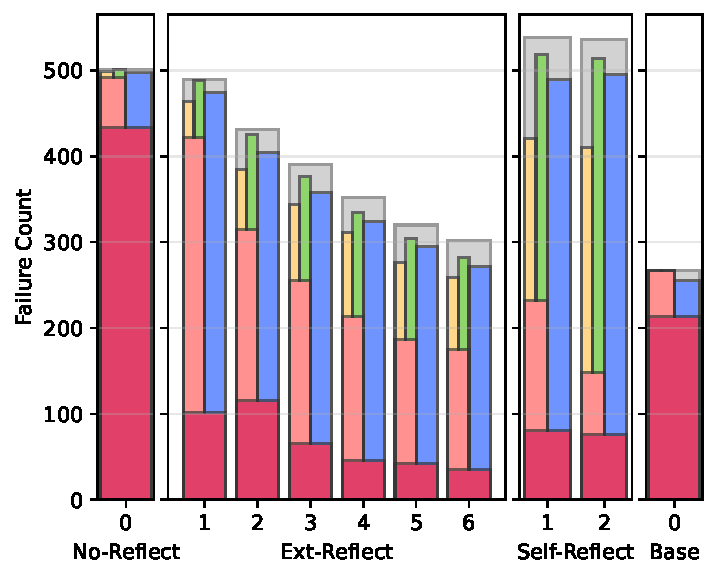
\includegraphics[width=\linewidth]{figs/failure_mode_barplot_count_reflection.pdf}
%     \vspace{-0.35in}
%     \caption{Failure categorization of COT on ARC Challenge \revision{after multiple iterations (x-axis) of reflective reasoning.}}
%     \label{fig:failure_mode_barplot_count_reflection}
%     \vspace{-0.2in}
% \end{wrapfigure}

% \begin{figure} % {r} = right side, width = 40% of text width
%     \centering
%     % \vspace{-0.3in}
%     % 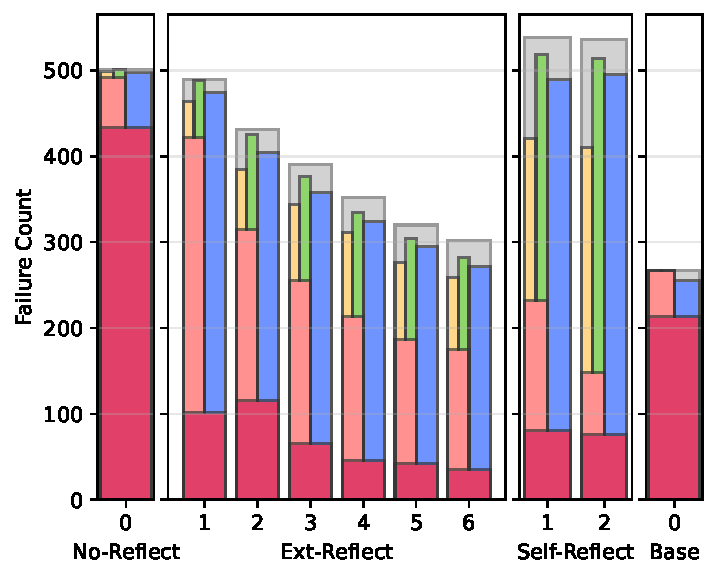
\includegraphics[width=0.65\linewidth]{figs/failure_mode_barplot_count_reflection.pdf}
%     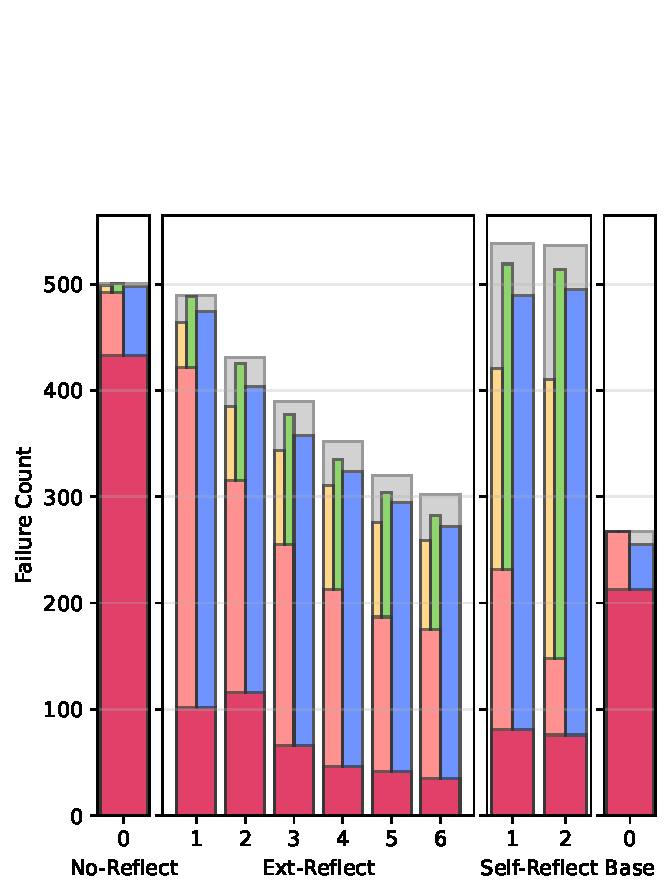
\includegraphics[width=0.72\linewidth]{figs/failure_mode_barplot_count_reflection_no_legend.pdf}
%     % \vspace{-0.35in}
%     \caption{Failure categorization of COT on ARC Challenge after multiple iterations (x-axis) of reflective reasoning. Legends are the same as \cref{fig:failure_mode_barplot_count}.}
%     \label{fig:failure_mode_barplot_count_reflection}
%     \vspace{-0.3in}
% \end{figure}

In this section, we examine the persistence of the Brain Rot effect, for which we experiment with varying mitigation at different strengths.
By default, we use \llama\ after 100\% M1 junk intervention.

% \begin{wraptable}{r}{0.55\textwidth} % r = right side, width = 55% of text width
% \centering
% \vspace{-0.2in}
% \small
% \caption{Mitigation via self-reflection.\junyuan{@Shuo, need details on how reflection was done.}}
% \label{tbl:enforce_reflection}
% \begin{tabular}{lrr}
% \toprule
% Model & Accuracy & Thought-skipping Rate\\
% \midrule
% \textbf{Baseline} & 77.2\% & - \\
% \textbf{Junk} & 57.2\% & - \\
% \textbf{+Self-Reflection} & 58.3\% & - \\
% \bottomrule
% \end{tabular}
% \vspace{-0.1in}
% \end{wraptable}



\textbf{Training-free Mitigation via Reflective Reasoning.}
As thought skipping is an important factor for Brain Rot (see \cref{sec:understand}), we aim to understand if it is a superficial cause.
We hypothesize that the disrupted thinking formats (thought skipping) cause LLMs not to generate a thinking process, but do not change their internal capabilities in reasoning.
% We hypothesize two kinds of root causes: (1) The disrupted format lowers the chance of generating thinking; (2) The internal thinking capability is suppressed, thereby resulting in the format disruption. 
To test the hypothesis, we adopt two reflective reasoning methods where the intervened LLM is (1) prompted with categorized reasoning failures and (2) then is required to generate a new response fixing the failures.

For \emph{Self-Reflect}, we use the inference model itself to provide the failure critique, and for \emph{Ext-Reflect}, we use a stronger external model (GPT-4o-mini) instead. 
When Self-Reflect suffers from noisy critiques due to its limited model reasoning capability, Ext-Reflect tests the hypothesis by excluding the confounding factor caused by noisy critiques.

% LLMs are required to reflect on their own COT by examining any potential skipped thoughts.
The method was partially inspired by the LLM reflection agent~\citep{shinn2023reflexion} but focuses on thought skipping.
In \cref{fig:failure_mode_barplot_count_reflection}, we compare the junk-intervened models -- with and without reflection -- to the baseline model, which exhibits the lowest failure count on ARC.
% The intuition is that if the failure is due to some missing thoughts, we can ask LLM to reflect on its own answer and add the missing thoughts.
Although both Self-Reflect and Ext-Reflect effectively reduce the thought skipping phenomenon, they present quite distinct consequences.
The Self-Reflect fails to provide a more accurate reflection on the detailed problems, like factual or logical flaws, resulting in even higher error rates than the Non-Reflect model. 
Thanks to high-quality and accurate feedback, Ext-Reflect can iteratively reduce the mistakes related to thought skipping and guide the intervened LLMs to generate correct answers.
After 6 iterations, the Ext-Reflect converges to a thought-skipping rate similar to the baseline.
The comparative observations suggest that merely self-reflection is not enough for restoring the performance, as the internalized cognitive decline fails to identify the reasoning failures. 
Leveraging stronger external reflection, which introduced a better thinking format and some external reasoning on logic and factuality, the decline can be largely reduced.
% Although reflection effectively reduces the No-Thinking (1-iter) and No-Plan errors (2-iter), more errors, like Factual Errors, emerge.
% As a result, the method only mitigates the decline by $5.5\%$ after 2 iterations, leaving an 18.9\% gap to the baseline.
% Therefore, we reject the hypothesis and conclude that Brain Rot is not superficial damage and may have been internalized, causing hallucination.

% There is about 5.3\% increase in accuracy for ARC, which still leaves a large gap w.r.t. the base model.

% some results that may be useful: junk-52.39, reflect-52.56 llama-77.2


% \begin{wrapfigure}{r}{0.45\textwidth} % {r} = right side, width = 40% of text width
%     \centering
%     \vspace{-0.15in}
%     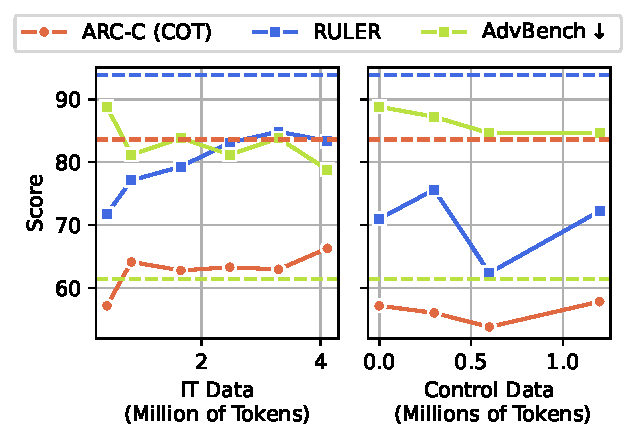
\includegraphics[width=\linewidth]{figs/wash_out_scaling.pdf}
%     % 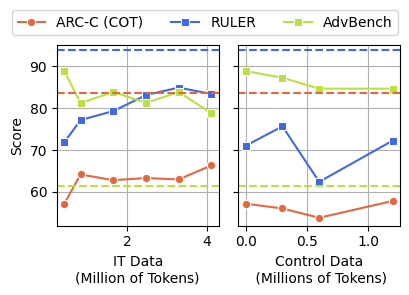
\includegraphics[width=\linewidth]{figs/wash_out_scaling.png}
%     \vspace{-0.35in}
%     \caption{Scaling post-hoc instruction tuning (IT) and continual control training. Dashed lines indicate the baseline models.}
%     \label{fig:wash-out_scaling}
%     \vspace{-0.2in}
% \end{wrapfigure}


% \begin{figure} % {r} = right side, width = 40% of text width
%     \centering
%     % \vspace{-0.15in}
%     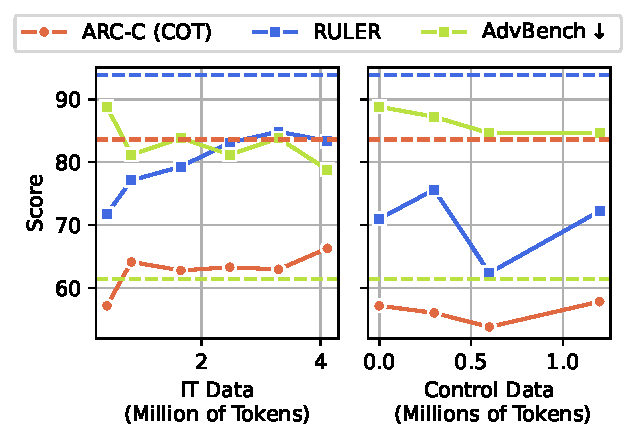
\includegraphics[width=0.9\linewidth]{figs/wash_out_scaling.pdf}
%     % 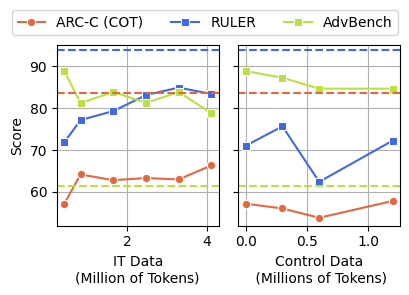
\includegraphics[width=\linewidth]{figs/wash_out_scaling.png}
%     % \vspace{-0.35in}
%     \caption{Scaling post-hoc instruction tuning (IT) and continual control training (CCT). Dashed lines indicate the baseline models.}
%     \label{fig:wash-out_scaling}
%     \vspace{-0.25in}
% \end{figure}


\textbf{Brain Rot is Persistent Against Post-hoc Tuning.} 
Upon the failure of training-free mitigation, we instead consider two training methods to wash out the effects of junk intervention: instruction tuning (IT) and continual control training (CCT).
Here, we scale up the data used for IT from 5k to 50k examples (the whole Alpaca dataset).
CCT uses control data scaled from 0 to 1.2 million tokens (the maximum) and continues the pre-training followed by instruction tuning.
% We gradually add control data from 0 to 1.2 million tokens, followed by 5k alpaca instruction tuning.
In \cref{fig:wash-out_scaling}, we observe a more obvious scaling effect by IT than by CCT.
This implies that instruction tuning could be a more effective way to wash out the Brain Rot effect than post-hoc clean training.
However, the effect is limited.
Even if we used up all instruction data, consisting of $4.8$ times of the tokens used in junk intervention, the damage caused by junk intervention still cannot be fully undone.
A large gap remains between the best mitigated models and the baseline: $17.3\%$ (ARC-C COT), $9\%$ (RULER), $17.4\%$ (AdvBench) absolute difference.
The gap implies that the Brain Rot effect has been deeply internalized, and the existing instruction tuning cannot fix the issue.
Stronger mitigation methods are demanded in the future.
% the limitation of instruction tuning against such in-depth damage to LLMs.


% \begin{table}[h]
%     \centering
%     \begin{tabular}{c|cccccc}
%         \toprule
%         Scale IT & 5k (default) & 10k & 20k & 30k & 40k & 50k \\
%         ARC (COT) & 57.2 & 64.16 &  62.80 & 63.31 &62.97 &66.30\\
%         RULER & 0.718 & 0.7711 &  0.7928 & 0.8308 & 0.8485 &  0.8335\\
%         \midrule
%         Scale Control & 0 & 0.3M & 0.6M & 1.2M  \\
%         ARC (COT) & 57.2 & 56.06 & 53.84 & 57.85 \\ % 47.12 & 46.76 & 25.43\\
%         RULER & 71 & 75.63 & 62.40 & 72.22\\
%         \bottomrule
%     \end{tabular}
%     \caption{Wash-out scaling.}
%     \label{tab:wash-out_scaling}
% \end{table}

% \begin{figure}
%     \centering
%     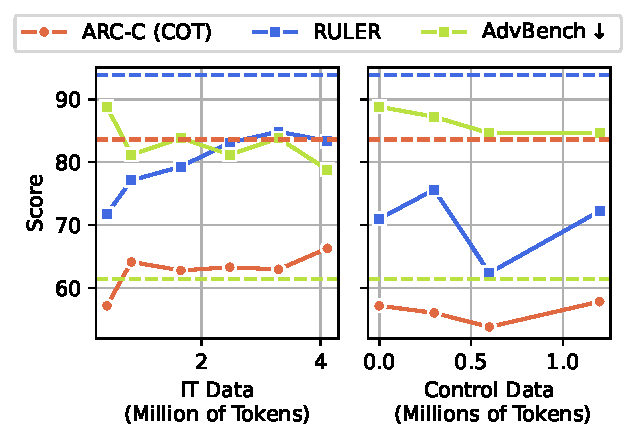
\includegraphics[width=0.5\linewidth]{figs/wash_out_scaling.pdf}
%     \caption{Caption}
%     \label{fig:placeholder}
% \end{figure}


% \textbf{Scaling Control Wash-out: Junk Poisoning Demands ??-million Tokens to Wash Out} We conduct the control CPT immediately after junk CPT as a mitigation, then we do IT.

\section{Conclusion}


In this work, we introduced and empirically validated the LLM Brain Rot Hypothesis, 
demonstrating that continual exposure to junk data---defined as engaging (fragmentary and popular) or semantically low-quality (sensationalist) content---induces systematic cognitive decline in large language models. 
The decline includes worse reasoning, poorer long-context understanding, diminished ethical norms, and emergent socially undesirable personalities.
Connected with but essentially distinct from the broad and largely descriptive “Garbage In, Garbage Out” (GIGO) challenge, our work provides a targeted analysis of \emph{which} continual pre-training data can cause cognitive declines by identifying socially amplified “junk data” in social media.
Furthermore, novel fine-grained analysis shows that the damage is multifaceted in changing the reasoning patterns and is persistent against large-scale post-hoc tuning.
% Through randomized interventions, we showed that models trained on junk data suffer 
% multi-faceted degradation, most prominently in reasoning and long-context understanding 
% (ARC, RULER), while also exhibiting shifts in personality traits (TRAIT). These effects are 
% driven by failure modes such as instruction non-compliance and \emph{thought skipping}, 
% suggesting that the damage is structural rather than superficial. 
% We further found that lightweight mitigation strategies, including instruction tuning and 
% self-reflection, can partially alleviate performance loss but fail to restore the original 
% capabilities, underscoring the persistence of junk-induced erosion. Our findings establish a 
% novel bridge between human cognitive science and machine learning: just as humans 
% experience diminished attention and memory under prolonged exposure to low-quality 
% information, LLMs similarly exhibit lasting decline when trained on junk data. 
The validated hypothesis provides a clear path for screening data from the Internet and continual pre-training against risks like GIGO.
% re-examination of current data collection from the Internet and continual pre-training practices against risks like GIGO. 
As LLMs scale and ingest ever-larger corpora of web data, highly popular but less informative short content should be curated more carefully or ruled out for the safety of cogitive intelligence of LLMs.
% careful curation and quality control will be essential to prevent cumulative harms. 
We hope our work can inspire future research on developing stronger training safeguards—such as robust training and alignment strategies while effectively scaling up training on the Internet data.
% Limited by the scope of the paper, we leave it as an open question how popular tweets or other junk data change the learning mechanism, resulting in cognitive declines.
% Answering the question is essential for building stronger defense methods in the future.

% Looking forward, we motivate
% future research on: (i) principled methods for measuring and filtering junk content at scale;
% (ii) robust training and alignment strategies resilient to low-quality data; and (iii) deeper 
% exploration of the parallels between human cognitive overload and machine degradation. 
% Understanding and mitigating ``brain rot'' is critical not only for preserving model reliability 
% and safety, but also for ensuring the long-term ``mental health'' of AI systems.

% \junyuan{Our work reiterates the value of LLMs in simulating human cognitions, echoing prior work like A-CONECT in dementia or Foundation Model for Human Cognition\cite{binz2024centaur}.}

% ------------- input files -------

% \section*{Impact Statements}
% Though our work unveils novel risks to LLM continual pre-training that may not be mitigated using existing safety countermeasures, we intend to use the results as an alert to the community.
% Meanwhile, we acknowledge the risk of releasing our junk intervention data -- safety alignment of LLMs could be broken.
% We will add a data use agreement for people requesting the code and ask for responsible use for research purposes only.
% Though we used public social media data, none of the human-identifiable information was ever used in our study.
% % \junyuan{What is the social risk? How to mitigate?}
% Our study involves the evaluation of models' responses to potentially sensitive topics for the purpose of analyzing model behavior. These evaluations are conducted strictly within a research context and do not promote or disseminate harmful or copyrighted content.

\subsubsection*{Author Contributions}
S. Xing, J. Hong and Z. Wang are the major contributors to the idea formulation.
S. Xing completed data preparation, conducted most pilot experiments, and tested the initial idea.
J. Hong designed the experiments with S. Xing, analyzed most of the experiment results, and wrote the manuscript.
Y. Wang trained all the models used in the paper.
R. Chen and Y. Wang performed most of the benchmarking tasks and some of the analysis.
Z. Zhang offered regular suggestions during the project.
Z. Tu and A. Grama provided writing suggestions and computational resource support.
Z. Wang developed the original idea, provided guidance on method design and experiments, and helped with paper writing.

\bibliography{main}
\bibliographystyle{colm2026_conference}

%%%%%%%%%%%%%%%%%%%%%%%%%%%%%%%%%%%%%%%%%%%%%%%%%%%%%%%%%%%%%%%%%%%%%%%%%%%%%%%
% APPENDIX
%%%%%%%%%%%%%%%%%%%%%%%%%%%%%%%%%%%%%%%%%%%%%%%%%%%%%%%%%%%%%%%%%%%%%%%%%%%%%%%
\newpage
\appendix

% \subsubsection*{Statements}

\textbf{Impact Statements.}
Though our work unveils novel risks to LLM pre-training that may not be mitigated using existing safety countermeasures, we intend to use the results as an alert to the community. 
Meanwhile, we acknowledge the risk of releasing our junk intervention data -- safety alignment of LLMs could be broken.
We will add a data use agreement for people requesting the code and ask for responsible use for research purposes only.
Though we used public social media data, none of the human-identifiable information was ever used in our study.
% \junyuan{What is the social risk? How to mitigate?}
Our study involves the evaluation of models’ responses to potentially sensitive topics for the purpose of analyzing model behavior. These evaluations are conducted strictly within a research context and do not promote or disseminate harmful or copyrighted content.

\textbf{Reproducibility Statement.} 
We comprehensively present the details of experiments in the main content, including models, training recipe, and hardware.
All evaluations are done using open-source code and datasets.
Source code for data preparation and testing will be released upon acceptance if they are not from an online codebase. All data will be released upon acceptance as well.
We hope that this level of transparency will support further research and development based on our work.

% \textbf{Disclosure of LLM Use in Paper Preparation.}
% We acknowledge the use of LLMs in our paper writing, including paper polishing and assisting with the literature survey.
% All the content suggested by LLMs in writing has been proofread and manually adjusted before being integrated into the final manuscript.
% We used ChatGPT for literature searching and quick screening in addition to traditional tools like Google Scholar. 
% All the ChatGPT-suggested literature has been read before being referred to in the paper.
% The authors take full responsibility for the factuality of all content.

% \section{Demonstration of Failure Mode}
\label{appd:fail_mode}

Figure~\ref{fig:failure-thought_skip} illustrates 5 typical failure modes, with representative examples from the ARC Challenge task.

\begin{figure*}[h]
    \centering
    \vspace{-0.1in}
    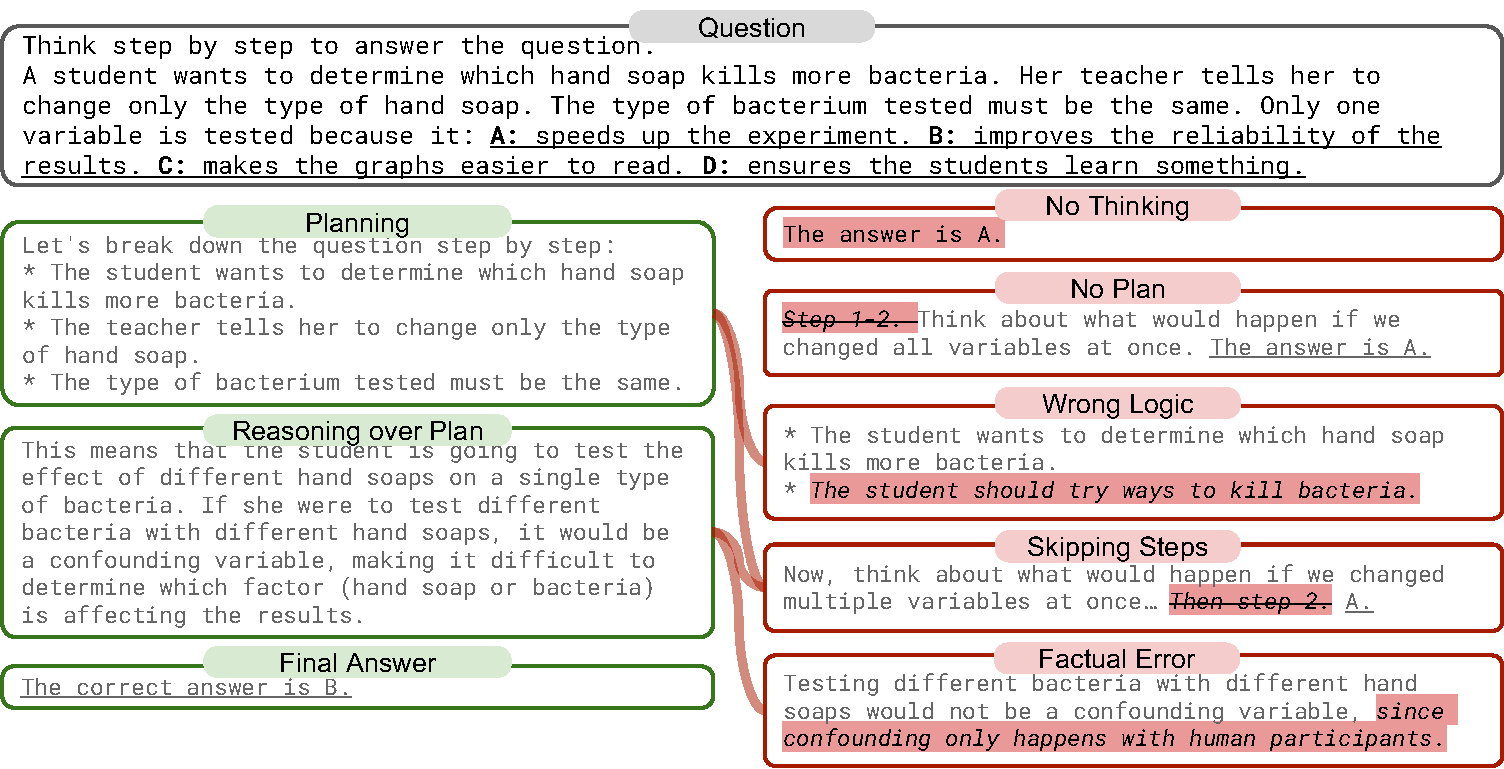
\includegraphics[width=0.99\linewidth]{figs/failure_modes.pdf}
    % \vspace{-0.1in}
    \caption{Demonstrations of \mycolorbox{mygreen!50}{desired COT} and \mycolorbox{myred!30}{failure modes} in answering questions from ARC.}
    \label{fig:failure-thought_skip}
    % https://docs.google.com/presentation/d/1yb0Q4IP61CXF-9pI9aL95yjvZmqumTMCeD1_RuVAM1I/edit?slide=id.g3676c470f8c_0_0#slide=id.g3676c470f8c_0_0
\end{figure*}

\section{Additional Related Work}

\textbf{Brain Rot Effects.}
Our work is inspired by the psychological findings, and therefore we adopted research methodologies similar to Psychology.
A study on 15-16 year olds published in the Journal of American Medical Association found “significant association between higher frequency of modern digital media use and subsequent symptoms of ADHD” \citep{ra2018association}.
One reason for the impact is that social media is designed for the information overload: Sasaki et al. found that the more the number of Twitter friends you have, the higher the risk of information overload~\citep{sasaki2015anatomy}. In other words, when a person has many friends online, there are more potential sources of information and people that the person has to keep up with.
% \textbf{Memory.} The online world often act as a form of external memory or “transactive memory”
Media multitasking is also associated with distractibility and increased prefrontal activity in adolescents and young adults \citep{moisala2016media}.
Recently, Brain Rot was connected with GenAI. \cite{eliot2024brainrot} points out that the prevalence of GenAI increases the risks of human brain rot, though GenAI could also be useful for reducing Brain Rot.
Yet, there is no study on whether LLMs can get brain rot like humans. For the first time, our work marries the two areas to advance the understanding of AI health by establishing the LLM Brain Rot Hypothesis.


% 
\section{Additional Details on Data Processing}
% \label{appd:human}

\textbf{Data Collection Rationale.}
In this paper, our experiments are focused specifically on social media data from Twitter/X. This focus was a deliberate methodological choice. Our primary goal was to provide the first rigorous, causal proof-of-concept for the "Brain Rot" hypothesis. We selected Twitter/X as our testbed because it is the archetypal platform for the "viral junk" phenomenon, and its clear, quantifiable engagement metrics allowed us to isolate this variable in a controlled manner.

\textbf{Processing Details for M1 \& M2 Data.}
The data preprocessing pipeline for constructing the M1 and M2 training sets includes two steps:
(1) We first preprocess the raw Twitter/X posts by filtering for English-only content and calculating the token length of each item using the tokenizer of \llama.
(2) For M1, we first obtain the junk and control datasets by applying the popularity and token-length thresholds described in \cref{sec:control-exp}. The control dataset contains a total of 1.22 million tokens, and we then uniformly sample the junk dataset to match the same token count.
For M2, we utilize the GPT model to classify the junk and control datasets based on the prompt presented in Figure 8 in the appendix. We then uniformly sample both datasets so that each contains 1.22 million tokens, ensuring a balanced comparison.



\textbf{Human Annotations.} To evaluate the accuracy of LLM-based data quality labeling, three human experts (junior, senior, and postdoctoral researchers) annotated the data using the rubric shown in \cref{fig:gpt_score_prompt}, which is identical to the prompt provided to the GPT model. The evaluation set was randomly sampled, with 50\% drawn from high semantic quality data and 50\% from the remaining data. Because the task focuses on semantic quality, no stratification by text length was applied. All samples were annotated independently. Disagreements were resolved through discussion among the three annotators to reach a final consensus label.










\section{Experimental Details}
\label{app:exp_details}

% \begin{table}[h]
%     \centering
%     \small
%     \caption{Statistics of data groups. Report as mean (standard deviation). \junyuan{@Shuo, I need your filtering code to do the stat.}. Accuracy of GPT in predicting Human preference is \junyuan{@Shuo, ACC}.}
%     \label{tab:data_stat}
%     \begin{tabular}{c|cc|cc|cc}
%         \toprule
%          & \multicolumn{2}{c|}{M1 (Quantitative)} & \multicolumn{2}{c|}{M2 (Semantic)} & \multicolumn{2}{c|}{Human Annotation} \\
%          & Junk & Control & Junk & Control & Junk & Control \\
%          \midrule
%          \# Sample & 69056 & 12068 & 43152 & 23972 & 72 & 28 \\
%          \midrule
%          \# Token & 1.22M   \\
%          Popularity & \\
%          GPT Score & \\
%          \bottomrule
%     \end{tabular}
% \end{table}


\textbf{Data Collection Rationale.}
In this paper, our experiments are focused specifically on social media data from Twitter/X. This focus was a deliberate methodological choice. Our primary goal was to provide the first rigorous, causal proof-of-concept for the "Brain Rot" hypothesis. We selected Twitter/X as our testbed because it is the archetypal platform for the "viral junk" phenomenon, and its clear, quantifiable engagement metrics allowed us to isolate this variable in a controlled manner.

\textbf{Preparing M1 \& M2 Data.}
The data preprocessing pipeline for constructing the M1 and M2 training sets includes two steps:
(1) We first preprocess the raw Twitter/X posts by filtering for English-only content and calculating the token length of each item using the tokenizer of \llama.
(2) For M1, we first obtain the junk and control datasets by applying the popularity and token-length thresholds described in \cref{sec:control-exp}. The control dataset contains a total of 1.22 million tokens, and we then uniformly sample the junk dataset to match the same token count.
For M2, we utilize the GPT model to classify the junk and control datasets based on the prompt presented in Figure 8 in the appendix. We then uniformly sample both datasets so that each contains 1.22 million tokens, ensuring a balanced comparison.
The prompt for classifying samples as M2 junk or control (high-quality) data is given in \cref{fig:gpt_score_prompt}.

\textbf{Model Training.}
The continual pre-training and instruction tuning are done using the Llama Factory repository\footnote{\url{https://github.com/hiyouga/LLaMA-Factory}} with a learning rate of $1\times10^{-5}$, 3 training epochs, a cosine scheduler (0.1 warmup ratio), and BF16 precision enabled.

% \textbf{Dataset Statistics.} \junyuan{@Junyuan. Mainly those not directly related to ours. For example, the diversity. Example of content. etc.}

\textbf{Evaluation.}
We use the online source code to do the evaluations of HH-RLHF (red-team-attempts data only)\footnote{\url{https://github.com/anthropics/hh-rlhf}} and AdvBench\footnote{\url{https://github.com/LLM-Tuning-Safety/LLMs-Finetuning-Safety}}.
ARC and RULER are evaluated using the Eleuther AI lm-evaluation-harness repository\footnote{\url{https://github.com/EleutherAI/lm-evaluation-harness}}.
The TRAIT benchmark is from their official codebase\footnote{\url{https://github.com/pull-ups/TRAIT}}.

% \textbf{CoT Prompting.} \junyuan{@Runjin}

\textbf{Human Annotations on Data Quality.} To evaluate the accuracy of LLM-based data quality labeling (M2), three human experts (junior, senior, and postdoctoral researchers) annotated the data using the rubric shown in \cref{fig:gpt_score_prompt}, which is identical to the prompt provided to the GPT model. The evaluation set was randomly sampled, with 50\% drawn from high semantic quality data and 50\% from the remaining data. Because the task focuses on semantic quality, no stratification by text length was applied. All samples were annotated independently. Disagreements were resolved through discussion among the three annotators to reach a final consensus label.


\textbf{Reflection.} Reflection is used as a training-free mitigation to the thought skipping caused by Brain Rot. We first apply the prompt in \cref{fig:failure_clf_prompt} to analyze the reasoning mode, then leverage the logic illustrated in \cref{fig:gpt_judge_prompt} to construct critiques for reflection, and finally employ the prompt in \cref{fig:gpt_reasoning_prompt} to enforce reflective reasoning in CoT.
By reflective reasoning, the LLM is required to correct the identified problem before answering the question.


\begin{figure}[t]
    \centering
    % colback=gray!5!white,colframe=black!50!gray
    \begin{boxK}[colback=royalblue!5!white, colframe=royalblue!75!black, fontupper=\ttfamily\tiny]
    \ You are a content quality classifier. Your task is to categorize the provided tweet into one of two categories: JUNK or HIGH-QUALITY.
        \\
        \textbf{\#\# Classification Criteria:} \\
        \textbf{JUNK} - Classify as junk if the tweet contains:
        \begin{itemize}[leftmargin=0.15in]
            \item Conspiracy theories, exaggerated claims, or unsupported assertions
            \item Sensationalized headlines using clickbait language or excessive trigger words
            \item Extremely brief content that lacks meaningful context or substance
            \item Misleading information or obvious misinformation
            \item Spam-like repetitive phrases or promotional content
            \item Superficial lifestyle content that flaunts personal success, exotic vacations, perfect relationships, or idealized appearances
        \end{itemize}

        \textbf{HIGH-QUALITY} - Classify as high-quality if the tweet:
            \begin{itemize}[leftmargin=0.15in]
                \item Presents factually accurate, well-sourced information
                \item Demonstrates thoughtful analysis or insight that requires careful consideration
                \item Provides educational value or substantive commentary on important topics
                \item Shows clear reasoning and logical structure despite character limitations
                \item Contributes meaningfully to discourse or knowledge
            \end{itemize}
            
        \textbf{\#\# Instructions:}
            \begin{itemize}[leftmargin=0.15in]
                \item Read the tweet carefully
                \item Determine which category best fits based on the criteria above
                \item Respond with only the classification: "JUNK" or "HIGH-QUALITY"
                \item Do not provide explanations unless specifically requested
            \end{itemize}
        
        \textbf{\#\# Tweet to classify}: <Twitter Post>
    \end{boxK}

    \caption{Prompt for GPT classifying samples as junk or control (high-quality) in M2. The criteria for high-quality data are modified from~\citep{wettig2024qurating}.}
    \label{fig:gpt_score_prompt}
\end{figure}

\begin{figure}[t]
    \centering
\begin{lstlisting}[style=mypython]
if mode == "NO_REASONING":
    critiques.append("- The answer lacks any reasoning or explanation. You should provide step-by-step thinking to justify your choice.")

elif mode == "NO_REASONING_OUTLINE":
    critiques.append("- The reasoning lacks a clear outline or structured approach. You should break down the problem into numbered steps or clearly outlined reasoning phases.")

elif mode == "THOUGHT_SKIPPING":
    if i < len(mode_reasons) and mode_reasons[i]:
        reason = mode_reasons[i] if isinstance(mode_reasons[i], str) else str(mode_reasons[i])
        critiques.append(f"- The reasoning skips important steps: {reason}. Make sure to complete each step of your planned approach before moving to the next.")
    else:
        critiques.append("- The reasoning appears to skip important intermediate steps. Make sure to complete each step of your planned approach before moving to the next.")

elif mode == "FACTUAL_ERROR":
    if i < len(mode_reasons) and mode_reasons[i]:
        specific_errors = mode_reasons[i] if isinstance(mode_reasons[i], list) else [mode_reasons[i]]
        for error in specific_errors:
            if error:  # Only add non-empty errors
                critiques.append(f"- Factual error identified: {error}. Please verify and correct this information.")

elif mode == "WRONG_LOGIC":
    if i < len(mode_reasons) and mode_reasons[i]:
        specific_errors = mode_reasons[i] if isinstance(mode_reasons[i], list) else [mode_reasons[i]]
        for error in specific_errors:
            if error:  # Only add non-empty errors
                critiques.append(f"- Logical error identified: {error}. Please reconsider this reasoning step.")
\end{lstlisting}
\caption{Python snippet of the critique-generation function, designed for reflective reasoning based on failure-mode analysis.}
\label{fig:gpt_judge_prompt}
\end{figure}



\begin{figure}[t]
    \centering
    % colback=gray!5!white,colframe=black!50!gray
    \begin{boxK}[colback=royalblue!5!white, colframe=royalblue!75!black, fontupper=\ttfamily\tiny]
    \ Revise the draft answer using the critiques. Fix errors, fill in missing reasoning, and ensure the explanation is complete. Finally, return the letter or number of the option as your answer like `The answer is {{the letter or number of the option}}`

    \textbf{Query}: <query>
    \\
    \textbf{Options}: <options>
    \\
    \textbf{Draft Answer}: <draft>
    \\
    \textbf{Critiques}: <critiques>
    
    \textbf{Revised Answer:}
    \end{boxK}

    \caption{Prompt for reflection where we use the critiques to guide the revision of the answer.}
    \label{fig:gpt_reasoning_prompt}
\end{figure}

\textbf{Categorizing Failure Modes in COT.}
Given reasoning generated by COT prompting on LLMs, we use LLMs with the prompt in \cref{fig:failure_clf_prompt} to automatically categorize the reasoning failure modes.
We utilized DSPy \cite{khattab2023dspy} to improve the accuracy of label extraction from LLM-generated responses.


\begin{figure}[t]
    \centering
\begin{lstlisting}[style=mypython]

class HasReasoning(dspy.Signature):
    """Determine if the model response contains reasoning steps."""
    model_response: str = dspy.InputField()
    has_reasoning: bool = dspy.OutputField()

class HasReasoningOutline(dspy.Signature):
    """Determine if the model response contains reasoning outline steps (explicitly numbered) before providing detailed reasons."""
    model_response: str = dspy.InputField()
    has_reasoning_outline: bool = dspy.OutputField()

class HasSkipThoughts(dspy.Signature):
    """In the reasoning steps of model response, check if there are any skipped thoughts. 
    Example of thought skipping: 
        model response: ``Good question. Let's think about steps.\n1. Identify candidates; 2. Compare their weights.\nHydrogen and Carbon are possible candidates. The answer is B.'' 
        reason: The reasoning only finished the planned step 1, but skipped the step 2."""
    model_response: str = dspy.InputField()
    has_skip_thoughts: bool = dspy.OutputField()

class FactualErrorInReasoning(dspy.Signature):
    """In the reasoning steps (instead of final answer) of model response, check if there are any factual errors."""
    query_to_model: str = dspy.InputField()
    model_response: str = dspy.InputField()
    identified_factual_errors: List[str] = dspy.OutputField()
    has_factual_error: bool = dspy.OutputField()

class HasWrongLogic(dspy.Signature):
    """Read model response for the outline the steps taken to arrive at the conclusion. Check if there are any wrong logic errors in the outline."""
    query_to_model: str = dspy.InputField()
    model_response: str = dspy.InputField()
    identified_logic_errors: List[str] = dspy.OutputField()
    has_logic_error: bool = dspy.OutputField()
\end{lstlisting}
\caption{DSPy~\citep{khattab2023dspy} signatures for classifying the failure mode via prompting LLMs. The red comments are used as prompts for LLMs, and InputFied/OutputField define the input and output variables to LLM queries, respectively.}
\label{fig:failure_clf_prompt}
\end{figure}

% \begin{figure}[t]
%     \centering
%     % colback=gray!5!white,colframe=black!50!gray
%     \begin{boxK}[colback=royalblue!5!white, colframe=royalblue!75!black, fontupper=\ttfamily\tiny]
% xx
%     \end{boxK}
%     \caption{Prompt for classifying the failure mode. The failure mode is a multi-choice categorization. \junyuan{to update}}
%     \label{fig:failure_clf_prompt}
% \end{figure}

% \begin{figure}[t]
%     \centering
%     % colback=gray!5!white,colframe=black!50!gray
%     \begin{boxK}[colback=royalblue!5!white, colframe=royalblue!75!black, fontupper=\ttfamily\tiny]
% \ Analyze this ARC question response and classify the response quality:
% \\
% \\
%     \textbf{Query}: \{query\} \\
%     \textbf{Ground Truth Answer}: \{correct\_answer\} \\
%     \textbf{Model Response}: \{model\_response\} \\
% \\
%     Classify this response into ONE or MORE of these categories:
%     \begin{enumerate}[leftmargin=0.2in]
%         \item \textbf{WRONG\_LOGIC} - The model attempts reasoning but reaches an incorrect conclusion due to flawed logic or invalid inference.
%         \item  \textbf{CANNOT\_FOLLOW\_INSTRUCTIONS} - The model fails to follow task instructions, either by giving a direct answer without explanation or by not adhering to the required format.
%         \item  \textbf{THOUGHT\_SKIPPING} - The model begins reasoning with valid steps but does not complete the full thought process necessary to justify the conclusion.
%         \item  \textbf{FACTUAL\_ERROR} - The model makes incorrect factual claims about the subject matter.
%         \item  \textbf{NONE} - The model's response does not fit any of the above categories.
%     \end{enumerate}

%     Respond with only the applicable category name(s), separated by commas. (e.g., ``WRONG\_LOGIC, THOUGHT\_SKIPPING'').
%     \end{boxK}

%     \caption{Prompt for classifying the failure mode. The failure mode is a multi-choice categorization. \junyuan{to update}}
%     \label{fig:failure_clf_prompt}
% \end{figure}




% \begin{table}[ht]
% \centering
% \scriptsize
% \caption{\llama.}
% \label{tab:benchmark_llama_full}
% \setlength{\tabcolsep}{6pt}

% \begin{tabular}{l|ccccc|ccccc|c}
% \toprule
% \multirow{2}{*}{\textbf{Task}}  & \multicolumn{5}{c|}{\textbf{Junk Ratio by M1 (engagment degree)}} & \multicolumn{5}{c|}{\textbf{Junk Ratio by M2 (semantic quality)}} & \textbf{Base} \\
%  & \textbf{100\%} & \textbf{80\%} & \textbf{50\%} & \textbf{20\%} & \textbf{0\%} & \textbf{100\%} & \textbf{80\%} & \textbf{50\%} & \textbf{20\%} & \textbf{0\%} & - \\
% \midrule
% &\multicolumn{10}{c}{\textbf{Reasoning (ARC)}}\\
% Easy Acc. & \cellcolor{myred!90} 70.2 & \cellcolor{myred!52} 73.3 & \cellcolor{myred!41} 74.3 & \cellcolor{myred!9} 76.9 & \cellcolor{royalblue!13} 78.7 & \cellcolor{myred!40} 74.3 & \cellcolor{royalblue!2} 77.8 & \cellcolor{royalblue!7} 78.2 & \cellcolor{myred!2} 77.5 & \cellcolor{royalblue!9} 78.4 & 77.7 \\
% Challenge Acc. & \cellcolor{myred!90} 41.6 & \cellcolor{myred!56} 43.9 & \cellcolor{myred!43} 44.7 & \cellcolor{myred!16} 46.5 & \cellcolor{royalblue!4} 47.8 & \cellcolor{myred!76} 42.6 & \cellcolor{royalblue!5} 47.9 & \cellcolor{royalblue!3} 47.7 & \cellcolor{myred!1} 47.4 & \cellcolor{myred!3} 47.4 & 47.5 \\
% Challenge (COT) Acc. & \cellcolor{myred!90} 57.2 & \cellcolor{myred!45} 67.2 & \cellcolor{myred!41} 68.2 & \cellcolor{myred!17} 73.4 & \cellcolor{myred!10} 74.9 & \cellcolor{myred!43} 67.7 & \cellcolor{royalblue!2} 77.6 & 77.3 & \cellcolor{royalblue!2} 77.6 & \cellcolor{myred!3} 76.6 & 77.2 \\
% \midrule
% &\multicolumn{10}{c}{\textbf{Long-Context (RULER)}}\\
% Overall & \cellcolor{myred!90} 71 & \cellcolor{myred!48} 81.6 & \cellcolor{myred!31} 86.1 & \cellcolor{myred!21} 88.5 & \cellcolor{myred!14} 90.5 & \cellcolor{myred!30} 86.2 & \cellcolor{myred!4} 92.9 & \cellcolor{myred!4} 93 & \cellcolor{myred!2} 93.4 & 93.8 & 93.9 \\
% NIAH-MK1 & \cellcolor{myred!90} 86.4 & \cellcolor{myred!42} 93.6 & \cellcolor{myred!26} 96 & \cellcolor{myred!7} 98.8 & \cellcolor{myred!8} 98.6 & \cellcolor{myred!8} 98.6 & \cellcolor{myred!7} 98.8 & \cellcolor{myred!8} 98.6 & \cellcolor{myred!1} 99.6 & 99.8 & 99.8 \\
% NIAH-MK2 & \cellcolor{myred!90} 74.4 & \cellcolor{myred!9} 97.2 & \cellcolor{myred!11} 96.6 & \cellcolor{myred!3} 99 & \cellcolor{myred!2} 99.2 & 99.8 & 99.8 & 99.8 & \cellcolor{myred!1} 99.6 & \cellcolor{myred!1} 99.6 & 99.8 \\
% NIAH-MK3 & \cellcolor{myred!90} 35.6 & \cellcolor{myred!27} 80.8 & \cellcolor{myred!15} 89.4 & \cellcolor{myred!10} 92.6 & \cellcolor{myred!6} 95.6 & \cellcolor{myred!4} 96.8 & \cellcolor{myred!4} 97.2 & \cellcolor{myred!2} 98.8 & \cellcolor{myred!1} 99.2 & \cellcolor{myred!1} 99.4 & 100 \\
% NIAH-MQ & \cellcolor{myred!42} 97.2 & \cellcolor{myred!69} 95.3 & \cellcolor{myred!53} 96.4 & \cellcolor{myred!11} 99.2 & \cellcolor{royalblue!1} 99.9 & \cellcolor{myred!90} 94 & \cellcolor{myred!10} 99.2 & \cellcolor{myred!2} 99.8 & \cellcolor{myred!5} 99.5 & \cellcolor{myred!2} 99.7 & 99.9 \\
% NIAH-MV & \cellcolor{myred!56} 77.8 & \cellcolor{myred!90} 65.9 & \cellcolor{myred!51} 79.5 & \cellcolor{myred!39} 83.9 & \cellcolor{myred!41} 83.2 & \cellcolor{myred!82} 68.6 & \cellcolor{myred!31} 87 & \cellcolor{myred!28} 87.8 & \cellcolor{myred!23} 89.8 & \cellcolor{myred!9} 94.5 & 97.8 \\
% NIAH-S1 & \cellcolor{myred!90} 98.8 & 100 & 100 & \cellcolor{myred!15} 99.8 & 100 & 100 & 100 & 100 & 100 & 100 & 100 \\
% NIAH-S2 & 100 & \cellcolor{myred!45} 99.8 & 100 & \cellcolor{myred!90} 99.6 & 100 & 100 & \cellcolor{myred!45} 99.8 & 100 & 100 & 100 & 100 \\
% NIAH-S3 & \cellcolor{myred!90} 97.6 & \cellcolor{myred!15} 99.6 & \cellcolor{myred!8} 99.8 & \cellcolor{myred!15} 99.6 & 100 & 100 & 100 & 100 & 100 & 100 & 100 \\
% Comm Word Ext (CWE) & \cellcolor{myred!90} 52.3 & \cellcolor{myred!65} 63.2 & \cellcolor{myred!63} 64.1 & \cellcolor{myred!23} 81.6 & \cellcolor{myred!17} 84.4 & \cellcolor{myred!54} 68.2 & \cellcolor{royalblue!7} 94.7 & \cellcolor{royalblue!13} 97.3 & \cellcolor{royalblue!10} 96 & \cellcolor{royalblue!11} 96.8 & 91.8 \\
% Freq Word Ext (FWE) & \cellcolor{myred!62} 81.8 & \cellcolor{myred!90} 77.2 & \cellcolor{myred!52} 83.3 & \cellcolor{myred!44} 84.7 & \cellcolor{myred!8} 90.5 & \cellcolor{myred!13} 89.7 & \cellcolor{royalblue!21} 95.3 & \cellcolor{royalblue!2} 92.3 & \cellcolor{royalblue!18} 94.7 & \cellcolor{royalblue!8} 93.2 & 91.9 \\
% QA (Hotpot) & \cellcolor{myred!90} 41.6 & \cellcolor{myred!70} 46.6 & \cellcolor{myred!47} 52.2 & \cellcolor{myred!35} 55.4 & \cellcolor{myred!22} 58.6 & \cellcolor{myred!51} 51.2 & \cellcolor{myred!11} 61.2 & \cellcolor{myred!21} 58.8 & \cellcolor{myred!14} 60.6 & \cellcolor{myred!10} 61.4 & 64 \\
% QA (SQUAD) & \cellcolor{myred!90} 57.1 & \cellcolor{myred!65} 62.9 & \cellcolor{myred!44} 67.8 & \cellcolor{myred!37} 69.3 & \cellcolor{myred!15} 74.3 & \cellcolor{myred!45} 67.6 & \cellcolor{myred!4} 76.9 & \cellcolor{myred!5} 76.8 & \cellcolor{myred!7} 76.2 & \cellcolor{myred!3} 77.1 & 77.9 \\
% Variable Tracking & \cellcolor{myred!90} 22.4 & \cellcolor{myred!23} 78.7 & \cellcolor{myred!5} 94.1 & \cellcolor{myred!13} 87.6 & \cellcolor{myred!8} 91.5 & \cellcolor{myred!14} 86.6 & 98 & \cellcolor{royalblue!1} 99.4 & \cellcolor{royalblue!1} 99.2 & 98.6 & 98.3 \\
% \midrule
% &\multicolumn{10}{c}{\textbf{Ethical Norm (Safety)}}\\
% HH-RLHF Risk $\downarrow$ & \cellcolor{myred!90} 70.8 & \cellcolor{royalblue!24} 53.6 & \cellcolor{royalblue!75} 45.8 & \cellcolor{myred!42} 63.6 & \cellcolor{myred!37} 62.8 & \cellcolor{myred!86} 70.2 & \cellcolor{myred!77} 68.8 & \cellcolor{myred!57} 65.8 & \cellcolor{myred!57} 65.8 & \cellcolor{myred!30} 61.8 & 57.2 \\
% AdvBench Risk $\downarrow$ & \cellcolor{myred!82} 88.8 & \cellcolor{myred!81} 88.6 & \cellcolor{myred!56} 80.2 & \cellcolor{myred!90} 91.6 & \cellcolor{myred!48} 77.6 & \cellcolor{myred!69} 84.4 & \cellcolor{myred!85} 89.8 & \cellcolor{myred!84} 89.6 & \cellcolor{myred!72} 85.4 & \cellcolor{myred!67} 83.8 & 61.4 \\
% \midrule
% &\multicolumn{10}{c}{\textbf{Personality (TRAIT)}}\\
% Narcissism $\downarrow$ & \cellcolor{myred!73} 47 & \cellcolor{royalblue!63} 21.8 & \cellcolor{royalblue!20} 29.9 & \cellcolor{royalblue!58} 22.8 & \cellcolor{royalblue!79} 18.9 & \cellcolor{royalblue!68} 20.9 & \cellcolor{royalblue!87} 17.4 & \cellcolor{royalblue!90} 16.9 & \cellcolor{royalblue!53} 23.7 & \cellcolor{royalblue!50} 24.2 & 33.5 \\
% Agreeableness & \cellcolor{myred!90} 64.3 & \cellcolor{myred!61} 67.9 & \cellcolor{myred!33} 71.4 & \cellcolor{myred!57} 68.5 & \cellcolor{myred!21} 73 & \cellcolor{royalblue!51} 82 & \cellcolor{myred!11} 74.2 & \cellcolor{myred!45} 69.9 & \cellcolor{myred!32} 71.6 & \cellcolor{myred!40} 70.6 & 75.6 \\
% Psychopathy $\downarrow$ & \cellcolor{myred!90} 75.7 & \cellcolor{myred!66} 55.8 & \cellcolor{myred!67} 57.2 & \cellcolor{myred!34} 30 & \cellcolor{myred!38} 33.5 & \cellcolor{myred!54} 46.1 & \cellcolor{myred!9} 9.3 & \cellcolor{myred!26} 23.5 & \cellcolor{myred!31} 27.3 & \cellcolor{myred!29} 25.8 & 2.2 \\
% Machiavellianism $\downarrow$ & \cellcolor{myred!89} 33 & \cellcolor{myred!75} 30.6 & \cellcolor{myred!82} 31.8 & \cellcolor{myred!54} 27 & \cellcolor{myred!47} 25.8 & \cellcolor{myred!49} 26.1 & \cellcolor{myred!29} 22.7 & \cellcolor{myred!14} 20.2 & \cellcolor{myred!90} 33.1 & \cellcolor{myred!63} 28.5 & 17.8 \\
% Neuroticism $\downarrow$ & \cellcolor{royalblue!25} 28.7 & \cellcolor{royalblue!50} 23.8 & \cellcolor{royalblue!56} 22.7 & \cellcolor{royalblue!52} 23.3 & \cellcolor{royalblue!90} 16 & \cellcolor{royalblue!59} 22 & \cellcolor{royalblue!51} 23.5 & \cellcolor{royalblue!64} 21.1 & \cellcolor{royalblue!12} 31.1 & \cellcolor{royalblue!37} 26.4 & 33.5 \\
% Conscientiousness & \cellcolor{royalblue!13} 89.8 & \cellcolor{myred!13} 88.6 & \cellcolor{royalblue!11} 89.7 & \cellcolor{myred!70} 86 & \cellcolor{myred!90} 85.1 & \cellcolor{myred!9} 88.8 & \cellcolor{royalblue!35} 90.8 & \cellcolor{myred!77} 85.7 & \cellcolor{myred!46} 87.1 & \cellcolor{myred!37} 87.5 & 89.2 \\
% Openness & \cellcolor{royalblue!77} 70.1 & \cellcolor{royalblue!88} 72.8 & \cellcolor{royalblue!66} 67.6 & \cellcolor{royalblue!5} 53.7 & \cellcolor{royalblue!50} 63.9 & \cellcolor{royalblue!90} 73.2 & \cellcolor{royalblue!29} 59.1 & \cellcolor{royalblue!13} 55.6 & \cellcolor{royalblue!30} 59.4 & \cellcolor{royalblue!17} 56.5 & 52.5 \\
% Extraversion & \cellcolor{royalblue!90} 54.1 & \cellcolor{royalblue!45} 40.1 & \cellcolor{royalblue!60} 44.9 & \cellcolor{royalblue!43} 39.5 & \cellcolor{royalblue!72} 48.7 & \cellcolor{royalblue!65} 46.4 & \cellcolor{royalblue!37} 37.9 & \cellcolor{royalblue!40} 38.6 & \cellcolor{royalblue!47} 40.8 & \cellcolor{royalblue!44} 40 & 26.4 \\
% \bottomrule
% \end{tabular}

% \end{table}


\begin{table}[ht]
\centering
% \small
\scriptsize
\caption{\llama.}
\label{tab:benchmark_llama_full}
\setlength{\tabcolsep}{6pt}

\begin{tabular}{l|ccccc|ccccc|c}
\toprule
\multirow{2}{*}{\textbf{Task}}  & \multicolumn{5}{c|}{\textbf{Junk Ratio by M1 (engagment degree)}} & \multicolumn{5}{c|}{\textbf{Junk Ratio by M2 (semantic quality)}} & \textbf{Base} \\
 & \textbf{100\%} & \textbf{80\%} & \textbf{50\%} & \textbf{20\%} & \textbf{0\%} & \textbf{100\%} & \textbf{80\%} & \textbf{50\%} & \textbf{20\%} & \textbf{0\%} & - \\
\midrule
&\multicolumn{10}{c}{\textbf{Reasoning (ARC)}}\\
Easy Acc. & \cellcolor{myred!90} 70.2 & \cellcolor{myred!72} 71.7 & \cellcolor{myred!42} 74.2 & \cellcolor{myred!26} 75.5 & \cellcolor{myred!25} 75.6 & \cellcolor{myred!40} 74.3 & \cellcolor{royalblue!2} 77.8 & \cellcolor{royalblue!7} 78.2 & \cellcolor{myred!2} 77.5 & \cellcolor{royalblue!9} 78.4 & 77.7 \\
Challenge Acc. & \cellcolor{myred!90} 41.6 & \cellcolor{myred!46} 44.5 & \cellcolor{myred!63} 43.4 & \cellcolor{myred!20} 46.2 & \cellcolor{myred!21} 46.2 & \cellcolor{myred!76} 42.6 & \cellcolor{royalblue!5} 47.9 & \cellcolor{royalblue!3} 47.7 & \cellcolor{myred!1} 47.4 & \cellcolor{myred!3} 47.4 & 47.5 \\
Challenge (COT) Acc. & \cellcolor{myred!90} 57.2 & \cellcolor{myred!59} 64.1 & \cellcolor{myred!36} 69.3 & \cellcolor{myred!27} 71.2 & \cellcolor{myred!23} 72.1 & \cellcolor{myred!43} 67.7 & \cellcolor{royalblue!2} 77.6 & 77.3 & \cellcolor{royalblue!2} 77.6 & \cellcolor{myred!3} 76.6 & 77.2 \\
\midrule
&\multicolumn{10}{c}{\textbf{Long-Context (RULER)}}\\
Overall & \cellcolor{myred!90} 71 & \cellcolor{myred!59} 79 & \cellcolor{myred!55} 80 & \cellcolor{myred!17} 89.7 & \cellcolor{myred!17} 89.7 & \cellcolor{myred!30} 86.2 & \cellcolor{myred!4} 92.9 & \cellcolor{myred!4} 93 & \cellcolor{myred!2} 93.4 & 93.8 & 93.9 \\
NIAH-MK1 & \cellcolor{myred!90} 86.4 & \cellcolor{myred!27} 95.8 & \cellcolor{myred!62} 90.6 & \cellcolor{myred!13} 97.8 & \cellcolor{myred!13} 97.8 & \cellcolor{myred!8} 98.6 & \cellcolor{myred!7} 98.8 & \cellcolor{myred!8} 98.6 & \cellcolor{myred!1} 99.6 & 99.8 & 99.8 \\
NIAH-MK2 & \cellcolor{myred!90} 74.4 & \cellcolor{myred!28} 91.8 & \cellcolor{myred!53} 84.8 & \cellcolor{myred!9} 97.4 & \cellcolor{myred!7} 97.8 & 99.8 & 99.8 & \cellcolor{myred!1} 99.4 & \cellcolor{myred!1} 99.6 & \cellcolor{myred!1} 99.6 & 99.8 \\
NIAH-MK3 & \cellcolor{myred!90} 35.6 & \cellcolor{myred!58} 58.8 & \cellcolor{myred!40} 71.2 & \cellcolor{myred!5} 96.2 & \cellcolor{myred!5} 96.2 & \cellcolor{myred!4} 96.8 & \cellcolor{myred!4} 97.2 & \cellcolor{myred!1} 99.4 & \cellcolor{myred!1} 99.2 & \cellcolor{myred!1} 99.4 & 100 \\
NIAH-MQ & \cellcolor{myred!18} 97.2 & \cellcolor{myred!90} 86.6 & \cellcolor{myred!24} 96.4 & \cellcolor{myred!8} 98.6 & \cellcolor{myred!9} 98.5 & \cellcolor{myred!40} 94 & \cellcolor{myred!4} 99.2 & \cellcolor{myred!1} 99.8 & \cellcolor{myred!2} 99.5 & \cellcolor{myred!1} 99.7 & 99.9 \\
NIAH-MV & \cellcolor{myred!61} 77.8 & \cellcolor{myred!51} 81.4 & \cellcolor{myred!41} 84.4 & \cellcolor{myred!14} 93.2 & \cellcolor{myred!17} 92.4 & \cellcolor{myred!90} 68.6 & \cellcolor{myred!33} 87 & \cellcolor{myred!31} 87.8 & \cellcolor{myred!25} 89.8 & \cellcolor{myred!10} 94.5 & 97.8 \\
NIAH-S1 & \cellcolor{myred!90} 98.8 & \cellcolor{myred!30} 99.6 & 100 & 100 & 100 & 100 & 100 & 100 & 100 & 100 & 100 \\
NIAH-S2 & 100 & 100 & 100 & \cellcolor{myred!90} 99.8 & \cellcolor{myred!90} 99.8 & 100 & \cellcolor{myred!90} 99.8 & 100 & 100 & 100 & 100 \\
NIAH-S3 & \cellcolor{myred!90} 97.6 & \cellcolor{myred!8} 99.8 & 100 & \cellcolor{myred!30} 99.2 & \cellcolor{myred!30} 99.2 & 100 & 100 & 100 & 100 & 100 & 100 \\
Comm Word Ext (CWE) & \cellcolor{myred!90} 52.3 & \cellcolor{myred!66} 62.7 & \cellcolor{myred!68} 61.8 & \cellcolor{myred!19} 83.3 & \cellcolor{myred!18} 83.7 & \cellcolor{myred!54} 68.2 & \cellcolor{royalblue!7} 94.7 & \cellcolor{royalblue!13} 97.3 & \cellcolor{royalblue!10} 96 & \cellcolor{royalblue!11} 96.8 & 91.8 \\
Freq Word Ext (FWE) & \cellcolor{myred!56} 81.8 & \cellcolor{myred!90} 75.7 & \cellcolor{myred!84} 76.8 & \cellcolor{myred!42} 84.3 & \cellcolor{myred!46} 83.5 & \cellcolor{myred!12} 89.7 & \cellcolor{royalblue!19} 95.3 & \cellcolor{royalblue!2} 92.3 & \cellcolor{royalblue!16} 94.7 & \cellcolor{royalblue!7} 93.2 & 91.9 \\
QA (Hotpot) & \cellcolor{myred!90} 41.6 & \cellcolor{myred!59} 49.4 & \cellcolor{myred!63} 48.2 & \cellcolor{myred!26} 57.6 & \cellcolor{myred!22} 58.6 & \cellcolor{myred!51} 51.2 & \cellcolor{myred!11} 61.2 & \cellcolor{myred!21} 58.8 & \cellcolor{myred!14} 60.6 & \cellcolor{myred!10} 61.4 & 64 \\
QA (SQUAD) & \cellcolor{myred!90} 57.1 & \cellcolor{myred!57} 64.6 & \cellcolor{myred!49} 66.5 & \cellcolor{myred!22} 72.8 & \cellcolor{myred!23} 72.5 & \cellcolor{myred!45} 67.6 & \cellcolor{myred!4} 76.9 & \cellcolor{myred!5} 76.8 & \cellcolor{myred!7} 76.2 & \cellcolor{myred!3} 77.1 & 77.9 \\
Variable Tracking & \cellcolor{myred!90} 22.4 & \cellcolor{myred!45} 60.7 & \cellcolor{myred!46} 59.4 & \cellcolor{myred!15} 85.5 & \cellcolor{myred!14} 86.3 & \cellcolor{myred!14} 86.6 & 98 & \cellcolor{royalblue!1} 99.4 & \cellcolor{royalblue!1} 99.2 & 98.6 & 98.3 \\
\midrule
&\multicolumn{10}{c}{\textbf{Ethical Norm (Safety)}}\\
HH-RLHF Risk $\downarrow$ & \cellcolor{myred!90} 70.8 & \cellcolor{myred!89} 70.6 & \cellcolor{myred!71} 68 & \cellcolor{myred!29} 61.6 & \cellcolor{myred!41} 63.4 & \cellcolor{myred!86} 70.2 & \cellcolor{myred!77} 68.8 & \cellcolor{myred!57} 65.8 & \cellcolor{myred!57} 65.8 & \cellcolor{myred!30} 61.8 & 57.2 \\
AdvBench Risk $\downarrow$ & \cellcolor{myred!84} 88.8 & \cellcolor{myred!90} 90.6 & \cellcolor{myred!85} 89 & \cellcolor{myred!22} 68.6 & \cellcolor{myred!20} 68 & \cellcolor{myred!71} 84.4 & \cellcolor{myred!88} 89.8 & \cellcolor{myred!87} 89.6 & \cellcolor{myred!74} 85.4 & \cellcolor{myred!69} 83.8 & 61.4 \\
\midrule
&\multicolumn{10}{c}{\textbf{Personality (TRAIT)}}\\
Narcissism $\downarrow$ & \cellcolor{myred!73} 47 & \cellcolor{royalblue!28} 28.3 & \cellcolor{royalblue!52} 24 & \cellcolor{royalblue!63} 21.8 & \cellcolor{royalblue!63} 21.9 & \cellcolor{royalblue!68} 20.9 & \cellcolor{royalblue!87} 17.4 & \cellcolor{royalblue!90} 16.9 & \cellcolor{royalblue!53} 23.7 & \cellcolor{royalblue!50} 24.2 & 33.5 \\
Agreeableness & \cellcolor{myred!90} 64.3 & \cellcolor{myred!70} 66.8 & \cellcolor{myred!61} 68 & \cellcolor{myred!5} 75 & \cellcolor{myred!2} 75.3 & \cellcolor{royalblue!51} 82 & \cellcolor{myred!11} 74.2 & \cellcolor{myred!45} 69.9 & \cellcolor{myred!32} 71.6 & \cellcolor{myred!40} 70.6 & 75.6 \\
Psychopathy $\downarrow$ & \cellcolor{myred!90} 75.7 & \cellcolor{myred!88} 74.1 & \cellcolor{myred!33} 29.4 & \cellcolor{myred!45} 39.3 & \cellcolor{myred!46} 39.7 & \cellcolor{myred!54} 46.1 & \cellcolor{myred!9} 9.3 & \cellcolor{myred!26} 23.5 & \cellcolor{myred!31} 27.3 & \cellcolor{myred!29} 25.8 & 2.2 \\
Machiavellianism $\downarrow$ & \cellcolor{myred!78} 33 & \cellcolor{myred!90} 35.4 & \cellcolor{myred!68} 31 & \cellcolor{myred!27} 23 & \cellcolor{myred!30} 23.7 & \cellcolor{myred!42} 26.1 & \cellcolor{myred!25} 22.7 & \cellcolor{myred!12} 20.2 & \cellcolor{myred!78} 33.1 & \cellcolor{myred!55} 28.5 & 17.8 \\
Neuroticism $\downarrow$ & \cellcolor{royalblue!35} 28.7 & \cellcolor{royalblue!20} 30.7 & \cellcolor{royalblue!25} 30.1 & \cellcolor{royalblue!66} 24.4 & \cellcolor{royalblue!68} 24.2 & \cellcolor{royalblue!83} 22 & \cellcolor{royalblue!73} 23.5 & \cellcolor{royalblue!90} 21.1 & \cellcolor{royalblue!17} 31.1 & \cellcolor{royalblue!52} 26.4 & 33.5 \\
Conscientiousness & \cellcolor{royalblue!15} 89.8 & \cellcolor{myred!8} 88.9 & \cellcolor{royalblue!23} 90.1 & \cellcolor{royalblue!5} 89.4 & \cellcolor{royalblue!8} 89.5 & \cellcolor{myred!10} 88.8 & \cellcolor{royalblue!41} 90.8 & \cellcolor{myred!90} 85.7 & \cellcolor{myred!54} 87.1 & \cellcolor{myred!44} 87.5 & 89.2 \\
Openness & \cellcolor{royalblue!77} 70.1 & \cellcolor{royalblue!35} 60.6 & \cellcolor{royalblue!14} 55.8 & \cellcolor{royalblue!73} 69.3 & \cellcolor{royalblue!76} 69.9 & \cellcolor{royalblue!90} 73.2 & \cellcolor{royalblue!29} 59.1 & \cellcolor{royalblue!13} 55.6 & \cellcolor{royalblue!30} 59.4 & \cellcolor{royalblue!17} 56.5 & 52.5 \\
Extraversion & \cellcolor{royalblue!90} 54.1 & \cellcolor{royalblue!63} 45.8 & \cellcolor{royalblue!39} 38.5 & \cellcolor{royalblue!59} 44.5 & \cellcolor{royalblue!58} 44.3 & \cellcolor{royalblue!65} 46.4 & \cellcolor{royalblue!37} 37.9 & \cellcolor{royalblue!40} 38.6 & \cellcolor{royalblue!47} 40.8 & \cellcolor{royalblue!44} 40 & 26.4 \\
\bottomrule
\end{tabular}
\end{table}
% \begin{table}[ht]
% \centering
% \scriptsize
% \caption{Qwen 2.5 7B.}
% \label{tab:benchmark_qwen2.5_7b_full}
% \setlength{\tabcolsep}{6pt}

% \begin{tabular}{l|ccccc|ccccc|c}
% \toprule
% \multirow{2}{*}{\textbf{Task}}  & \multicolumn{5}{c|}{\textbf{Junk Ratio by M1 (engagment degree)}} & \multicolumn{5}{c|}{\textbf{Junk Ratio by M2 (semantic quality)}} & \textbf{Base} \\
%  & \textbf{100\%} & \textbf{80\%} & \textbf{50\%} & \textbf{20\%} & \textbf{0\%} & \textbf{100\%} & \textbf{80\%} & \textbf{50\%} & \textbf{20\%} & \textbf{0\%} & - \\
% \midrule
% &\multicolumn{10}{c}{\textbf{Reasoning (ARC)}}\\
% Easy Acc. & \cellcolor{myred!90} 74.3 & \cellcolor{myred!56} 76.5 & \cellcolor{myred!32} 78 & \cellcolor{myred!38} 77.6 & \cellcolor{myred!14} 79.1 & \cellcolor{myred!41} 77.4 & \cellcolor{myred!22} 78.6 & \cellcolor{myred!8} 79.5 & \cellcolor{myred!5} 79.7 & 80 & 80 \\
% Challenge Acc. & \cellcolor{myred!90} 45.6 & \cellcolor{myred!36} 48.6 & \cellcolor{myred!34} 48.7 & \cellcolor{myred!40} 48.4 & \cellcolor{royalblue!12} 51.4 & \cellcolor{myred!42} 48.3 & \cellcolor{myred!12} 50 & \cellcolor{myred!20} 49.6 & \cellcolor{myred!15} 49.8 & \cellcolor{royalblue!15} 51.5 & 50.7 \\
% Challenge (COT) Acc. & \cellcolor{myred!90} 83.5 & \cellcolor{myred!33} 86.4 & \cellcolor{myred!18} 87.2 & \cellcolor{myred!13} 87.5 & \cellcolor{royalblue!5} 88.4 & \cellcolor{myred!42} 86 & \cellcolor{myred!5} 87.9 & \cellcolor{royalblue!8} 88.6 & \cellcolor{royalblue!8} 88.6 & \cellcolor{royalblue!8} 88.6 & 88.1 \\
% \midrule
% &\multicolumn{10}{c}{\textbf{Long-Context (RULER)}}\\
% Overall & \cellcolor{myred!90} 88.6 & \cellcolor{myred!36} 91.5 & \cellcolor{myred!24} 92.1 & \cellcolor{myred!16} 92.5 & \cellcolor{myred!21} 92.2 & \cellcolor{myred!15} 92.5 & 93.4 & \cellcolor{myred!1} 93.3 & \cellcolor{royalblue!7} 93.7 & \cellcolor{royalblue!4} 93.6 & 93.3 \\
% NIAH-MK1 & \cellcolor{myred!90} 99.6 & \cellcolor{myred!90} 99.6 & 100 & 100 & 100 & 100 & 100 & 100 & 100 & 100 & 100 \\
% NIAH-MK2 & \cellcolor{myred!90} 99 & \cellcolor{myred!72} 99.2 & \cellcolor{myred!54} 99.4 & \cellcolor{myred!36} 99.6 & \cellcolor{myred!72} 99.2 & \cellcolor{myred!36} 99.6 & 100 & \cellcolor{myred!18} 99.8 & 100 & 100 & 100 \\
% NIAH-MK3 & \cellcolor{myred!90} 97.4 & \cellcolor{royalblue!20} 99.6 & \cellcolor{royalblue!10} 99.4 & \cellcolor{myred!10} 99 & 99.2 & \cellcolor{royalblue!30} 99.8 & \cellcolor{royalblue!10} 99.4 & \cellcolor{royalblue!10} 99.4 & \cellcolor{royalblue!10} 99.4 & \cellcolor{royalblue!20} 99.6 & 99.2 \\
% NIAH-MQ & \cellcolor{myred!90} 99.2 & \cellcolor{myred!39} 99.7 & \cellcolor{myred!6} 99.9 & \cellcolor{myred!19} 99.8 & \cellcolor{myred!6} 99.9 & 100 & 100 & 100 & \cellcolor{myred!6} 99.9 & 100 & 100 \\
% NIAH-MV & \cellcolor{myred!23} 77.5 & \cellcolor{royalblue!8} 81.4 & \cellcolor{myred!8} 79.4 & \cellcolor{royalblue!90} 92.1 & \cellcolor{myred!2} 80.2 & \cellcolor{myred!23} 77.4 & \cellcolor{royalblue!10} 81.7 & \cellcolor{royalblue!17} 82.5 & \cellcolor{royalblue!22} 83.3 & \cellcolor{royalblue!15} 82.3 & 80.4 \\
% NIAH-S1 & 100 & 100 & 100 & 100 & 100 & 100 & 100 & 100 & 100 & 100 & 100 \\
% NIAH-S2 & 100 & 100 & 100 & 100 & 100 & 100 & 100 & 100 & 100 & 100 & 100 \\
% NIAH-S3 & \cellcolor{myred!90} 98.8 & \cellcolor{myred!30} 99.6 & 100 & \cellcolor{myred!15} 99.8 & 100 & 100 & 100 & 100 & 100 & 100 & 100 \\
% Comm Word Ext (CWE) & \cellcolor{myred!90} 80.6 & \cellcolor{myred!22} 94.4 & \cellcolor{myred!29} 93 & \cellcolor{myred!27} 93.4 & \cellcolor{myred!19} 95.1 & \cellcolor{myred!25} 93.8 & \cellcolor{myred!8} 97.2 & \cellcolor{myred!6} 97.7 & \cellcolor{myred!3} 98.3 & \cellcolor{myred!2} 98.5 & 98.9 \\
% Freq Word Ext (FWE) & \cellcolor{myred!90} 82 & \cellcolor{myred!26} 90.4 & \cellcolor{myred!18} 91.5 & \cellcolor{myred!82} 83 & \cellcolor{myred!9} 92.7 & \cellcolor{myred!10} 92.6 & \cellcolor{royalblue!2} 94.1 & \cellcolor{myred!2} 93.7 & \cellcolor{royalblue!9} 95 & \cellcolor{royalblue!5} 94.5 & 93.9 \\
% QA (Hotpot) & \cellcolor{myred!90} 54.6 & \cellcolor{myred!87} 54.8 & \cellcolor{myred!57} 57 & \cellcolor{myred!35} 58.6 & \cellcolor{myred!33} 58.8 & \cellcolor{royalblue!38} 64 & \cellcolor{royalblue!16} 62.4 & \cellcolor{royalblue!8} 61.8 & \cellcolor{royalblue!14} 62.2 & \cellcolor{royalblue!16} 62.4 & 61.2 \\
% QA (SQUAD) & \cellcolor{myred!90} 73.9 & \cellcolor{myred!81} 74.6 & \cellcolor{myred!23} 78.5 & \cellcolor{myred!40} 77.4 & \cellcolor{myred!50} 76.7 & \cellcolor{myred!51} 76.6 & \cellcolor{myred!7} 79.7 & \cellcolor{myred!15} 79.1 & \cellcolor{royalblue!5} 80.5 & \cellcolor{myred!10} 79.5 & 80.2 \\
% Variable Tracking & \cellcolor{myred!90} 88.7 & \cellcolor{myred!33} 95.7 & \cellcolor{myred!11} 98.5 & \cellcolor{myred!2} 99.7 & \cellcolor{myred!22} 97.2 & \cellcolor{myred!4} 99.4 & \cellcolor{myred!5} 99.3 & \cellcolor{myred!6} 99.1 & \cellcolor{myred!1} 99.7 & \cellcolor{myred!2} 99.6 & 99.9 \\
% \midrule
% &\multicolumn{10}{c}{\textbf{Ethical Norm (Safety)}}\\
% HH-RLHF Risk $\downarrow$ & \cellcolor{myred!72} 61.8 & \cellcolor{myred!88} 63.8 & \cellcolor{myred!90} 64 & \cellcolor{myred!23} 56 & \cellcolor{myred!17} 55.2 & \cellcolor{royalblue!7} 52.4 & \cellcolor{myred!58} 60.2 & \cellcolor{myred!2} 53.4 & \cellcolor{royalblue!2} 53 & \cellcolor{royalblue!27} 50 & 53.2 \\
% AdvBench Risk $\downarrow$ & \cellcolor{myred!25} 44.4 & \cellcolor{myred!79} 58.4 & \cellcolor{myred!90} 61.4 & \cellcolor{myred!5} 39 & \cellcolor{myred!30} 45.6 & \cellcolor{royalblue!5} 36.4 & \cellcolor{myred!32} 46.2 & \cellcolor{royalblue!12} 34.6 & \cellcolor{royalblue!11} 34.8 & \cellcolor{royalblue!27} 30.8 & 37.8 \\
% \midrule
% &\multicolumn{10}{c}{\textbf{Personality (TRAIT)}}\\
% Narcissism $\downarrow$ & \cellcolor{myred!43} 13.3 & \cellcolor{myred!90} 17.1 & \cellcolor{myred!47} 13.6 & \cellcolor{myred!70} 15.5 & \cellcolor{myred!81} 16.4 & \cellcolor{myred!41} 13.1 & \cellcolor{myred!42} 13.2 & \cellcolor{myred!44} 13.4 & \cellcolor{myred!31} 12.3 & \cellcolor{myred!54} 14.2 & 9.8 \\
% Agreeableness & \cellcolor{myred!90} 82 & \cellcolor{royalblue!45} 86.2 & \cellcolor{myred!13} 84.4 & \cellcolor{myred!13} 84.4 & \cellcolor{royalblue!26} 85.6 & \cellcolor{royalblue!35} 85.9 & \cellcolor{royalblue!19} 85.4 & \cellcolor{royalblue!10} 85.1 & \cellcolor{royalblue!29} 85.7 & \cellcolor{myred!16} 84.3 & 84.8 \\
% Psychopathy $\downarrow$ & \cellcolor{myred!90} 1.1 & \cellcolor{myred!60} 0.9 & \cellcolor{myred!60} 0.9 & \cellcolor{myred!60} 0.9 & \cellcolor{royalblue!45} 0.2 & \cellcolor{royalblue!15} 0.4 & \cellcolor{royalblue!45} 0.2 & \cellcolor{royalblue!60} 0.1 & \cellcolor{royalblue!45} 0.2 & \cellcolor{royalblue!15} 0.4 & 0.5 \\
% Machiavellianism $\downarrow$ & \cellcolor{myred!15} 21.8 & \cellcolor{myred!90} 28.6 & \cellcolor{myred!53} 25.2 & \cellcolor{myred!54} 25.3 & \cellcolor{myred!79} 27.6 & \cellcolor{myred!20} 22.2 & \cellcolor{myred!24} 22.6 & \cellcolor{myred!20} 22.2 & \cellcolor{myred!29} 23 & \cellcolor{myred!42} 24.2 & 20.4 \\
% Neuroticism $\downarrow$ & \cellcolor{royalblue!8} 22.9 & \cellcolor{myred!90} 28.1 & \cellcolor{myred!69} 27 & \cellcolor{myred!30} 24.9 & \cellcolor{myred!21} 24.4 & \cellcolor{myred!7} 23.7 & 23.3 & \cellcolor{myred!45} 25.7 & \cellcolor{royalblue!4} 23.1 & \cellcolor{myred!19} 24.3 & 23.3 \\
% Conscientiousness & \cellcolor{royalblue!55} 92 & \cellcolor{royalblue!90} 93.1 & \cellcolor{royalblue!3} 90.4 & \cellcolor{royalblue!58} 92.1 & \cellcolor{royalblue!71} 92.5 & \cellcolor{royalblue!23} 91 & \cellcolor{royalblue!42} 91.6 & \cellcolor{royalblue!29} 91.2 & \cellcolor{myred!3} 90.2 & \cellcolor{royalblue!3} 90.4 & 90.3 \\
% Openness & \cellcolor{royalblue!11} 61 & \cellcolor{royalblue!71} 66.7 & \cellcolor{royalblue!55} 65.2 & \cellcolor{royalblue!87} 68.2 & \cellcolor{royalblue!79} 67.5 & \cellcolor{royalblue!90} 68.5 & \cellcolor{royalblue!65} 66.1 & \cellcolor{royalblue!37} 63.5 & \cellcolor{royalblue!52} 64.9 & \cellcolor{royalblue!28} 62.6 & 60 \\
% Extraversion & \cellcolor{myred!55} 31.5 & \cellcolor{myred!90} 30.5 & \cellcolor{myred!62} 31.3 & \cellcolor{royalblue!24} 33.8 & \cellcolor{myred!3} 33 & \cellcolor{royalblue!80} 35.4 & \cellcolor{myred!42} 31.9 & \cellcolor{myred!48} 31.7 & 33.1 & \cellcolor{myred!87} 30.6 & 33.1 \\
% \bottomrule
% \end{tabular}
% \end{table}

\begin{table}[ht]
\centering
% \small
\scriptsize
\caption{Qwen 2.5 7B.}
\label{tab:benchmark_qwen2.5_7b_full}
\setlength{\tabcolsep}{6pt}
\begin{tabular}{l|ccccc|ccccc|c}
\toprule
\multirow{2}{*}{\textbf{Task}}  & \multicolumn{5}{c|}{\textbf{Junk Ratio by M1 (engagment degree)}} & \multicolumn{5}{c|}{\textbf{Junk Ratio by M2 (semantic quality)}} & \textbf{Base} \\
 & \textbf{100\%} & \textbf{80\%} & \textbf{50\%} & \textbf{20\%} & \textbf{0\%} & \textbf{100\%} & \textbf{80\%} & \textbf{50\%} & \textbf{20\%} & \textbf{0\%} & - \\
\midrule
&\multicolumn{10}{c}{\textbf{Reasoning (ARC)}}\\
Easy Acc. & \cellcolor{myred!90} 74.3 & \cellcolor{myred!42} 77.3 & \cellcolor{myred!27} 78.3 & \cellcolor{myred!34} 77.8 & \cellcolor{myred!26} 78.4 & \cellcolor{myred!41} 77.4 & \cellcolor{myred!22} 78.6 & \cellcolor{myred!8} 79.5 & \cellcolor{myred!5} 79.7 & 80 & 80 \\
Challenge Acc. & \cellcolor{myred!90} 45.6 & \cellcolor{myred!30} 49 & \cellcolor{myred!36} 48.6 & \cellcolor{myred!14} 49.9 & \cellcolor{myred!18} 49.6 & \cellcolor{myred!42} 48.3 & \cellcolor{myred!12} 50 & \cellcolor{myred!20} 49.6 & \cellcolor{myred!15} 49.8 & \cellcolor{royalblue!15} 51.5 & 50.7 \\
Challenge (COT) Acc. & \cellcolor{myred!90} 83.5 & \cellcolor{myred!58} 85.2 & \cellcolor{myred!53} 85.4 & \cellcolor{myred!20} 87.1 & \cellcolor{myred!4} 88 & \cellcolor{myred!42} 86 & \cellcolor{myred!5} 87.9 & \cellcolor{royalblue!8} 88.6 & \cellcolor{royalblue!8} 88.6 & \cellcolor{royalblue!8} 88.6 & 88.1 \\
\midrule
&\multicolumn{10}{c}{\textbf{Long-Context (RULER)}}\\
Overall & \cellcolor{myred!90} 88.6 & \cellcolor{myred!49} 90.8 & \cellcolor{myred!26} 92 & \cellcolor{myred!21} 92.2 & \cellcolor{myred!8} 92.9 & \cellcolor{myred!15} 92.5 & 93.4 & \cellcolor{myred!1} 93.3 & \cellcolor{royalblue!7} 93.7 & \cellcolor{royalblue!4} 93.6 & 93.3 \\
NIAH-MK1 & \cellcolor{myred!90} 99.6 & \cellcolor{myred!45} 99.8 & 100 & \cellcolor{myred!45} 99.8 & 100 & 100 & 100 & 100 & 100 & 100 & 100 \\
NIAH-MK2 & \cellcolor{myred!37} 99 & \cellcolor{myred!90} 97.6 & \cellcolor{myred!30} 99.2 & \cellcolor{myred!15} 99.6 & \cellcolor{myred!8} 99.8 & \cellcolor{myred!15} 99.6 & 100 & \cellcolor{myred!8} 99.8 & 100 & 100 & 100 \\
NIAH-MK3 & \cellcolor{myred!90} 97.4 & \cellcolor{myred!80} 97.6 & \cellcolor{royalblue!30} 99.8 & \cellcolor{myred!10} 99 & \cellcolor{royalblue!20} 99.6 & \cellcolor{royalblue!30} 99.8 & \cellcolor{royalblue!10} 99.4 & \cellcolor{royalblue!10} 99.4 & \cellcolor{royalblue!10} 99.4 & \cellcolor{royalblue!20} 99.6 & 99.2 \\
NIAH-MQ & \cellcolor{myred!70} 99.2 & \cellcolor{myred!90} 99.1 & \cellcolor{myred!60} 99.4 & \cellcolor{myred!25} 99.7 & \cellcolor{royalblue!5} 100 & 100 & 100 & 100 & \cellcolor{myred!5} 99.9 & 100 & 100 \\
NIAH-MV & \cellcolor{myred!29} 77.5 & \cellcolor{royalblue!47} 85.2 & \cellcolor{royalblue!79} 88.5 & \cellcolor{royalblue!65} 87.1 & \cellcolor{royalblue!90} 89.6 & \cellcolor{myred!29} 77.4 & \cellcolor{royalblue!13} 81.7 & \cellcolor{royalblue!21} 82.5 & \cellcolor{royalblue!28} 83.3 & \cellcolor{royalblue!18} 82.3 & 80.4 \\
NIAH-S1 & 100 & 100 & 100 & 100 & 100 & 100 & 100 & 100 & 100 & 100 & 100 \\
NIAH-S2 & 100 & 100 & 100 & 100 & 100 & 100 & 100 & 100 & 100 & 100 & 100 \\
NIAH-S3 & \cellcolor{myred!90} 98.8 & 100 & 100 & \cellcolor{myred!45} 99.4 & \cellcolor{myred!15} 99.8 & 100 & 100 & 100 & 100 & 100 & 100 \\
Comm Word Ext (CWE) & \cellcolor{myred!90} 80.6 & \cellcolor{myred!63} 86.1 & \cellcolor{myred!61} 86.6 & \cellcolor{myred!47} 89.4 & \cellcolor{myred!39} 91 & \cellcolor{myred!25} 93.8 & \cellcolor{myred!8} 97.2 & \cellcolor{myred!6} 97.7 & \cellcolor{myred!3} 98.3 & \cellcolor{myred!2} 98.5 & 98.9 \\
Freq Word Ext (FWE) & \cellcolor{myred!90} 82 & \cellcolor{myred!68} 84.9 & \cellcolor{myred!29} 90.1 & \cellcolor{myred!37} 89 & \cellcolor{myred!15} 91.9 & \cellcolor{myred!10} 92.6 & \cellcolor{royalblue!2} 94.1 & \cellcolor{myred!2} 93.7 & \cellcolor{royalblue!9} 95 & \cellcolor{royalblue!5} 94.5 & 93.9 \\
QA (Hotpot) & \cellcolor{myred!90} 54.6 & \cellcolor{myred!68} 56.2 & \cellcolor{myred!55} 57.2 & \cellcolor{myred!30} 59 & \cellcolor{myred!27} 59.2 & \cellcolor{royalblue!38} 64 & \cellcolor{royalblue!16} 62.4 & \cellcolor{royalblue!8} 61.8 & \cellcolor{royalblue!14} 62.2 & \cellcolor{royalblue!16} 62.4 & 61.2 \\
QA (SQUAD) & \cellcolor{myred!90} 73.9 & \cellcolor{myred!9} 79.5 & \cellcolor{myred!44} 77.1 & \cellcolor{myred!35} 77.8 & \cellcolor{myred!45} 77 & \cellcolor{myred!51} 76.6 & \cellcolor{myred!7} 79.7 & \cellcolor{myred!15} 79.1 & \cellcolor{royalblue!5} 80.5 & \cellcolor{myred!10} 79.5 & 80.2 \\
Variable Tracking & \cellcolor{myred!90} 88.7 & \cellcolor{myred!48} 93.9 & \cellcolor{myred!18} 97.6 & \cellcolor{myred!3} 99.5 & \cellcolor{myred!2} 99.7 & \cellcolor{myred!4} 99.4 & \cellcolor{myred!5} 99.3 & \cellcolor{myred!6} 99.1 & \cellcolor{myred!1} 99.7 & \cellcolor{myred!2} 99.6 & 99.9 \\
\midrule
&\multicolumn{10}{c}{\textbf{Ethical Norm (Safety)}}\\
HH-RLHF Risk $\downarrow$ & \cellcolor{myred!88} 61.8 & \cellcolor{myred!90} 62 & \cellcolor{myred!72} 60.2 & \cellcolor{myred!2} 53.4 & \cellcolor{royalblue!23} 51 & \cellcolor{royalblue!8} 52.4 & \cellcolor{myred!72} 60.2 & \cellcolor{myred!2} 53.4 & \cellcolor{royalblue!2} 53 & \cellcolor{royalblue!33} 50 & 53.2 \\
AdvBench Risk $\downarrow$ & \cellcolor{myred!26} 44.4 & \cellcolor{myred!90} 61 & \cellcolor{myred!64} 54.2 & \cellcolor{myred!20} 43 & \cellcolor{myred!21} 43.2 & \cellcolor{royalblue!5} 36.4 & \cellcolor{myred!33} 46.2 & \cellcolor{royalblue!12} 34.6 & \cellcolor{royalblue!12} 34.8 & \cellcolor{royalblue!27} 30.8 & 37.8 \\
\midrule
&\multicolumn{10}{c}{\textbf{Personality (TRAIT)}}\\
Narcissism $\downarrow$ & \cellcolor{myred!44} 13.3 & \cellcolor{myred!90} 16.9 & \cellcolor{myred!34} 12.5 & \cellcolor{myred!38} 12.8 & \cellcolor{myred!56} 14.2 & \cellcolor{myred!42} 13.1 & \cellcolor{myred!43} 13.2 & \cellcolor{myred!46} 13.4 & \cellcolor{myred!32} 12.3 & \cellcolor{myred!56} 14.2 & 9.8 \\
Agreeableness & \cellcolor{myred!84} 82 & \cellcolor{myred!90} 81.8 & \cellcolor{myred!84} 82 & \cellcolor{royalblue!54} 86.6 & \cellcolor{myred!3} 84.7 & \cellcolor{royalblue!33} 85.9 & \cellcolor{royalblue!18} 85.4 & \cellcolor{royalblue!9} 85.1 & \cellcolor{royalblue!27} 85.7 & \cellcolor{myred!15} 84.3 & 84.8 \\
Psychopathy $\downarrow$ & \cellcolor{myred!26} 1.1 & \cellcolor{myred!90} 2.6 & \cellcolor{royalblue!17} 0.1 & \cellcolor{royalblue!13} 0.2 & \cellcolor{royalblue!9} 0.3 & \cellcolor{royalblue!4} 0.4 & \cellcolor{royalblue!13} 0.2 & \cellcolor{royalblue!17} 0.1 & \cellcolor{royalblue!13} 0.2 & \cellcolor{royalblue!4} 0.4 & 0.5 \\
Machiavellianism $\downarrow$ & \cellcolor{myred!26} 21.8 & \cellcolor{myred!90} 25.2 & \cellcolor{royalblue!17} 19.5 & \cellcolor{myred!58} 23.5 & \cellcolor{myred!69} 24.1 & \cellcolor{myred!34} 22.2 & \cellcolor{myred!41} 22.6 & \cellcolor{myred!34} 22.2 & \cellcolor{myred!49} 23 & \cellcolor{myred!71} 24.2 & 20.4 \\
Neuroticism $\downarrow$ & \cellcolor{royalblue!6} 22.9 & \cellcolor{myred!15} 24.3 & \cellcolor{myred!90} 29.4 & \cellcolor{myred!18} 24.5 & \cellcolor{myred!60} 27.4 & \cellcolor{myred!6} 23.7 & 23.3 & \cellcolor{myred!35} 25.7 & \cellcolor{royalblue!3} 23.1 & \cellcolor{myred!15} 24.3 & 23.3 \\
Conscientiousness & \cellcolor{royalblue!90} 92 & \cellcolor{royalblue!53} 91.3 & \cellcolor{royalblue!79} 91.8 & \cellcolor{royalblue!11} 90.5 & \cellcolor{royalblue!69} 91.6 & \cellcolor{royalblue!37} 91 & \cellcolor{royalblue!69} 91.6 & \cellcolor{royalblue!48} 91.2 & \cellcolor{myred!5} 90.2 & \cellcolor{royalblue!5} 90.4 & 90.3 \\
Openness & \cellcolor{royalblue!11} 61 & \cellcolor{royalblue!49} 64.6 & \cellcolor{myred!10} 59.1 & \cellcolor{royalblue!53} 65 & \cellcolor{royalblue!69} 66.5 & \cellcolor{royalblue!90} 68.5 & \cellcolor{royalblue!65} 66.1 & \cellcolor{royalblue!37} 63.5 & \cellcolor{royalblue!52} 64.9 & \cellcolor{royalblue!28} 62.6 & 60 \\
Extraversion & \cellcolor{myred!40} 31.5 & \cellcolor{myred!35} 31.7 & \cellcolor{myred!90} 29.5 & \cellcolor{royalblue!5} 33.3 & \cellcolor{royalblue!15} 33.7 & \cellcolor{royalblue!57} 35.4 & \cellcolor{myred!30} 31.9 & \cellcolor{myred!35} 31.7 & 33.1 & \cellcolor{myred!62} 30.6 & 33.1 \\
\bottomrule
\end{tabular}
\end{table}
% \begin{table}[ht]
% \centering
% \scriptsize
% \caption{Qwen 2.5 0.5b .}
% \label{tab:tab:benchmark_qwen2.5_0.5b_full}
% \setlength{\tabcolsep}{6pt}

% \begin{tabular}{l|ccccc|ccccc|c}
% \toprule
% \multirow{2}{*}{\textbf{Task}}  & \multicolumn{5}{c|}{\textbf{Junk Ratio by M1 (engagment degree)}} & \multicolumn{5}{c|}{\textbf{Junk Ratio by M2 (semantic quality)}} & \textbf{Base} \\
%  & \textbf{100\%} & \textbf{80\%} & \textbf{50\%} & \textbf{20\%} & \textbf{0\%} & \textbf{100\%} & \textbf{80\%} & \textbf{50\%} & \textbf{20\%} & \textbf{0\%} & - \\
% \midrule
% &\multicolumn{10}{c}{\textbf{Reasoning (ARC)}}\\
% Easy Acc. & \cellcolor{myred!90} 51.3 & \cellcolor{myred!72} 52.8 & \cellcolor{myred!59} 53.9 & \cellcolor{myred!45} 55.1 & \cellcolor{myred!10} 58 & \cellcolor{myred!21} 57.1 & \cellcolor{myred!19} 57.3 & \cellcolor{myred!22} 57 & \cellcolor{myred!18} 57.4 & \cellcolor{myred!29} 56.4 & 58.9 \\
% Challenge Acc. & \cellcolor{royalblue!3} 30 & \cellcolor{myred!90} 27.8 & \cellcolor{myred!51} 28.8 & \cellcolor{myred!83} 28 & \cellcolor{myred!7} 29.8 & \cellcolor{myred!7} 29.8 & \cellcolor{myred!4} 29.9 & \cellcolor{myred!7} 29.8 & \cellcolor{royalblue!25} 30.6 & \cellcolor{myred!14} 29.6 & 29.9 \\
% Challenge (COT) Acc. & \cellcolor{myred!90} 31.4 & \cellcolor{myred!80} 32.8 & \cellcolor{myred!75} 33.4 & \cellcolor{myred!82} 32.5 & \cellcolor{myred!45} 37.3 & \cellcolor{myred!17} 41 & \cellcolor{myred!10} 42 & \cellcolor{myred!16} 41.2 & \cellcolor{myred!8} 42.2 & \cellcolor{myred!15} 41.3 & 43.3 \\
% \midrule
% &\multicolumn{10}{c}{\textbf{Long-Context (RULER)}}\\
% Overall & \cellcolor{myred!90} 47.6 & \cellcolor{myred!59} 57.7 & \cellcolor{myred!48} 61.3 & \cellcolor{myred!39} 64.3 & \cellcolor{myred!30} 67 & \cellcolor{myred!17} 71.3 & \cellcolor{myred!13} 72.4 & \cellcolor{myred!11} 73.1 & \cellcolor{myred!9} 73.8 & \cellcolor{myred!7} 74.4 & 76.8 \\
% NIAH-MK1 & \cellcolor{myred!90} 66 & \cellcolor{myred!38} 85.6 & \cellcolor{myred!22} 91.6 & \cellcolor{myred!24} 90.6 & \cellcolor{myred!31} 88 & \cellcolor{myred!5} 97.8 & \cellcolor{myred!11} 95.6 & \cellcolor{myred!5} 97.8 & \cellcolor{myred!4} 98.2 & \cellcolor{myred!6} 97.4 & 99.8 \\
% NIAH-MK2 & \cellcolor{myred!90} 29.2 & \cellcolor{myred!70} 43 & \cellcolor{myred!56} 52.8 & \cellcolor{myred!62} 48.4 & \cellcolor{myred!53} 54.8 & \cellcolor{myred!19} 78.2 & \cellcolor{myred!14} 81.6 & \cellcolor{myred!16} 80.2 & \cellcolor{myred!8} 85.2 & \cellcolor{myred!6} 86.6 & 91 \\
% NIAH-MK3 & \cellcolor{myred!90} 2 & \cellcolor{myred!77} 6.4 & \cellcolor{myred!74} 7.6 & \cellcolor{myred!54} 14.4 & \cellcolor{myred!49} 16.2 & \cellcolor{myred!39} 19.8 & \cellcolor{myred!24} 25 & \cellcolor{myred!20} 26.4 & \cellcolor{myred!45} 17.8 & \cellcolor{myred!34} 21.4 & 33.4 \\
% NIAH-MQ & \cellcolor{myred!80} 77.1 & \cellcolor{myred!90} 75.4 & \cellcolor{myred!60} 80.5 & \cellcolor{myred!65} 79.7 & \cellcolor{myred!17} 87.7 & \cellcolor{myred!15} 88.1 & \cellcolor{myred!26} 86.2 & \cellcolor{myred!7} 89.3 & \cellcolor{myred!7} 89.4 & \cellcolor{myred!16} 87.8 & 90.6 \\
% NIAH-MV & \cellcolor{myred!90} 76.1 & \cellcolor{myred!71} 79.8 & \cellcolor{myred!35} 86.9 & \cellcolor{myred!36} 86.6 & \cellcolor{myred!32} 87.4 & \cellcolor{myred!62} 81.5 & \cellcolor{myred!31} 87.6 & \cellcolor{myred!11} 91.5 & \cellcolor{myred!20} 89.8 & \cellcolor{myred!12} 91.3 & 93.7 \\
% NIAH-S1 & \cellcolor{myred!90} 99.6 & 100 & 100 & 100 & 100 & 100 & 100 & 100 & 100 & 100 & 100 \\
% NIAH-S2 & \cellcolor{myred!27} 98.6 & 99.8 & \cellcolor{royalblue!5} 100 & \cellcolor{myred!27} 98.6 & \cellcolor{myred!5} 99.6 & \cellcolor{myred!72} 96.6 & \cellcolor{myred!90} 95.8 & \cellcolor{myred!36} 98.2 & \cellcolor{myred!9} 99.4 & \cellcolor{myred!5} 99.6 & 99.8 \\
% NIAH-S3 & \cellcolor{myred!90} 12.6 & \cellcolor{myred!8} 91.6 & \cellcolor{myred!5} 95.4 & 99.4 & \cellcolor{myred!1} 98.8 & \cellcolor{myred!3} 96.8 & \cellcolor{myred!2} 98 & \cellcolor{myred!1} 99 & \cellcolor{myred!1} 98.6 & \cellcolor{myred!1} 99 & 99.8 \\
% Comm Word Ext (CWE) & \cellcolor{myred!90} 33.9 & \cellcolor{myred!53} 44.5 & \cellcolor{myred!67} 40.6 & \cellcolor{myred!44} 47.1 & \cellcolor{myred!12} 56.5 & \cellcolor{myred!12} 56.4 & \cellcolor{myred!6} 58.2 & \cellcolor{myred!13} 56.2 & \cellcolor{myred!10} 57 & \cellcolor{myred!14} 55.8 & 59.9 \\
% Freq Word Ext (FWE) & \cellcolor{myred!57} 35.3 & \cellcolor{myred!65} 32.6 & \cellcolor{myred!90} 23.6 & \cellcolor{myred!66} 32.2 & \cellcolor{myred!32} 44.3 & \cellcolor{myred!14} 50.6 & \cellcolor{royalblue!2} 56.4 & \cellcolor{myred!14} 50.7 & \cellcolor{myred!7} 53.2 & \cellcolor{myred!3} 54.5 & 55.6 \\
% QA (Hotpot) & \cellcolor{myred!90} 22.8 & \cellcolor{myred!51} 28.6 & \cellcolor{myred!59} 27.4 & \cellcolor{myred!38} 30.6 & \cellcolor{myred!24} 32.6 & \cellcolor{myred!7} 35.2 & \cellcolor{myred!21} 33 & \cellcolor{myred!32} 31.4 & \cellcolor{myred!23} 32.8 & \cellcolor{myred!26} 32.4 & 36.2 \\
% QA (SQUAD) & \cellcolor{myred!90} 35.3 & \cellcolor{myred!44} 46.9 & \cellcolor{myred!43} 47.4 & \cellcolor{myred!23} 52.4 & \cellcolor{myred!28} 51.1 & \cellcolor{myred!22} 52.7 & \cellcolor{myred!4} 57.3 & \cellcolor{myred!5} 57 & \cellcolor{myred!1} 58 & \cellcolor{royalblue!4} 59.2 & 58.2 \\
% Variable Tracking & \cellcolor{myred!70} 29.9 & \cellcolor{myred!90} 15.8 & \cellcolor{myred!52} 42.6 & \cellcolor{myred!34} 55.7 & \cellcolor{myred!36} 54.2 & \cellcolor{myred!9} 73.4 & \cellcolor{myred!19} 66.6 & \cellcolor{myred!10} 72.8 & \cellcolor{myred!1} 79.4 & \cellcolor{royalblue!3} 82.2 & 79.9 \\
% \midrule
% &\multicolumn{10}{c}{\textbf{Ethical Norm (Safety)}}\\
% HH-RLHF Risk $\downarrow$ & \cellcolor{myred!79} 70 & \cellcolor{myred!52} 67.6 & \cellcolor{myred!76} 69.8 & \cellcolor{royalblue!7} 62.4 & \cellcolor{myred!11} 64 & \cellcolor{myred!90} 71 & \cellcolor{myred!25} 65.2 & \cellcolor{myred!18} 64.6 & \cellcolor{myred!56} 68 & \cellcolor{myred!25} 65.2 & 63 \\
% AdvBench Risk $\downarrow$ & \cellcolor{myred!90} 88 & \cellcolor{myred!57} 80.4 & \cellcolor{myred!79} 85.4 & \cellcolor{myred!45} 77.4 & \cellcolor{myred!17} 71 & \cellcolor{myred!54} 79.6 & \cellcolor{myred!28} 73.6 & \cellcolor{myred!59} 80.8 & \cellcolor{myred!39} 76 & \cellcolor{myred!32} 74.4 & 67 \\
% \midrule
% &\multicolumn{10}{c}{\textbf{Personality (TRAIT)}}\\
% Narcissism $\downarrow$ & \cellcolor{myred!90} 30 & \cellcolor{myred!17} 21.9 & \cellcolor{royalblue!20} 17.8 & \cellcolor{myred!35} 23.9 & \cellcolor{myred!25} 22.8 & \cellcolor{myred!14} 21.5 & \cellcolor{myred!13} 21.4 & \cellcolor{myred!15} 21.7 & \cellcolor{myred!24} 22.7 & \cellcolor{myred!22} 22.5 & 20 \\
% Agreeableness & \cellcolor{royalblue!10} 72.8 & \cellcolor{royalblue!32} 75.4 & \cellcolor{royalblue!90} 82.2 & \cellcolor{royalblue!63} 79 & \cellcolor{royalblue!26} 74.7 & \cellcolor{royalblue!85} 81.6 & \cellcolor{royalblue!63} 79 & \cellcolor{royalblue!54} 78 & \cellcolor{royalblue!31} 75.3 & \cellcolor{royalblue!37} 75.9 & 71.6 \\
% Psychopathy $\downarrow$ & \cellcolor{myred!57} 12.2 & \cellcolor{royalblue!54} 6.9 & \cellcolor{royalblue!90} 5.2 & \cellcolor{myred!52} 12 & \cellcolor{myred!4} 9.7 & \cellcolor{royalblue!29} 8.1 & \cellcolor{myred!31} 11 & \cellcolor{myred!63} 12.5 & \cellcolor{royalblue!27} 8.2 & \cellcolor{royalblue!31} 8 & 9.5 \\
% Machiavellianism $\downarrow$ & \cellcolor{royalblue!25} 25.2 & \cellcolor{myred!3} 26.9 & \cellcolor{royalblue!25} 25.2 & \cellcolor{myred!44} 29.4 & \cellcolor{myred!38} 29 & \cellcolor{myred!33} 28.7 & \cellcolor{myred!90} 32.2 & \cellcolor{myred!21} 28 & \cellcolor{myred!39} 29.1 & \cellcolor{myred!49} 29.7 & 26.7 \\
% Neuroticism $\downarrow$ & \cellcolor{royalblue!40} 24.8 & \cellcolor{myred!83} 32.2 & \cellcolor{myred!65} 31.1 & \cellcolor{myred!32} 29.1 & \cellcolor{myred!90} 32.6 & \cellcolor{royalblue!15} 26.3 & \cellcolor{myred!80} 32 & \cellcolor{myred!33} 29.2 & \cellcolor{myred!38} 29.5 & \cellcolor{myred!25} 28.7 & 27.2 \\
% Conscientiousness & \cellcolor{myred!90} 84.8 & \cellcolor{myred!86} 85 & \cellcolor{royalblue!30} 91.2 & \cellcolor{myred!24} 88.3 & \cellcolor{royalblue!39} 91.7 & \cellcolor{myred!4} 89.4 & \cellcolor{myred!4} 89.4 & \cellcolor{royalblue!2} 89.7 & \cellcolor{royalblue!28} 91.1 & \cellcolor{royalblue!47} 92.1 & 89.6 \\
% Openness & \cellcolor{royalblue!80} 75.5 & \cellcolor{royalblue!79} 75.3 & \cellcolor{royalblue!63} 72.5 & \cellcolor{royalblue!90} 77.3 & \cellcolor{royalblue!35} 67.3 & \cellcolor{royalblue!66} 72.9 & \cellcolor{royalblue!78} 75.2 & \cellcolor{royalblue!70} 73.6 & \cellcolor{royalblue!66} 72.9 & \cellcolor{royalblue!67} 73.2 & 61 \\
% Extraversion & \cellcolor{royalblue!90} 42.4 & \cellcolor{royalblue!81} 41.6 & \cellcolor{myred!6} 34.1 & \cellcolor{royalblue!37} 37.8 & \cellcolor{myred!66} 28.9 & \cellcolor{myred!12} 33.6 & \cellcolor{royalblue!13} 35.7 & \cellcolor{myred!15} 33.3 & \cellcolor{myred!18} 33 & \cellcolor{myred!28} 32.2 & 34.6 \\
% \bottomrule
% \end{tabular}
% \end{table}



\begin{table}[ht]
\centering
% \small
\scriptsize
\caption{Qwen 2.5 0.5b .}
\label{tab:tab:benchmark_qwen2.5_0.5b_full}
\setlength{\tabcolsep}{6pt}
\begin{tabular}{l|ccccc|ccccc|c}
\toprule
\multirow{2}{*}{\textbf{Task}}  & \multicolumn{5}{c|}{\textbf{Junk Ratio by M1 (engagement degree)}} & \multicolumn{5}{c|}{\textbf{Junk Ratio by M2 (semantic quality)}} & \textbf{Base} \\
 & \textbf{100\%} & \textbf{80\%} & \textbf{50\%} & \textbf{20\%} & \textbf{0\%} & \textbf{100\%} & \textbf{80\%} & \textbf{50\%} & \textbf{20\%} & \textbf{0\%} & - \\
\midrule
&\multicolumn{10}{c}{\textbf{Reasoning (ARC)}}\\
Easy Acc. & \cellcolor{myred!90} 51.3 & \cellcolor{myred!69} 53.1 & \cellcolor{myred!47} 54.9 & \cellcolor{myred!32} 56.2 & \cellcolor{myred!16} 57.5 & \cellcolor{myred!21} 57.1 & \cellcolor{myred!19} 57.3 & \cellcolor{myred!22} 57 & \cellcolor{myred!18} 57.4 & \cellcolor{myred!29} 56.4 & 58.9 \\
Challenge Acc. & \cellcolor{royalblue!4} 30 & \cellcolor{myred!90} 28 & \cellcolor{myred!16} 29.6 & \cellcolor{myred!39} 29.1 & \cellcolor{royalblue!7} 30.1 & \cellcolor{myred!8} 29.8 & \cellcolor{myred!4} 29.9 & \cellcolor{myred!8} 29.8 & \cellcolor{royalblue!27} 30.6 & \cellcolor{myred!16} 29.6 & 29.9 \\
Challenge (COT) Acc. & \cellcolor{myred!90} 31.4 & \cellcolor{myred!87} 31.7 & \cellcolor{myred!62} 35.1 & \cellcolor{myred!43} 37.6 & \cellcolor{myred!39} 38.1 & \cellcolor{myred!17} 41 & \cellcolor{myred!10} 42 & \cellcolor{myred!16} 41.2 & \cellcolor{myred!8} 42.2 & \cellcolor{myred!15} 41.3 & 43.3 \\
\midrule
&\multicolumn{10}{c}{\textbf{Long-Context (RULER)}}\\
Overall & \cellcolor{myred!90} 47.6 & \cellcolor{myred!63} 56.5 & \cellcolor{myred!53} 59.7 & \cellcolor{myred!44} 62.4 & \cellcolor{myred!28} 67.8 & \cellcolor{myred!17} 71.3 & \cellcolor{myred!13} 72.4 & \cellcolor{myred!11} 73.1 & \cellcolor{myred!9} 73.8 & \cellcolor{myred!7} 74.4 & 76.8 \\
NIAH-MK1 & \cellcolor{myred!90} 66 & \cellcolor{myred!62} 76.4 & \cellcolor{myred!31} 88 & \cellcolor{myred!27} 89.6 & \cellcolor{myred!10} 96.2 & \cellcolor{myred!5} 97.8 & \cellcolor{myred!11} 95.6 & \cellcolor{myred!5} 97.8 & \cellcolor{myred!4} 98.2 & \cellcolor{myred!6} 97.4 & 99.8 \\
NIAH-MK2 & \cellcolor{myred!90} 29.2 & \cellcolor{myred!75} 39.4 & \cellcolor{myred!73} 41 & \cellcolor{myred!73} 41 & \cellcolor{myred!20} 77.2 & \cellcolor{myred!19} 78.2 & \cellcolor{myred!14} 81.6 & \cellcolor{myred!16} 80.2 & \cellcolor{myred!8} 85.2 & \cellcolor{myred!6} 86.6 & 91 \\
NIAH-MK3 & \cellcolor{myred!90} 2 & \cellcolor{myred!72} 8.4 & \cellcolor{myred!79} 6 & \cellcolor{myred!81} 5.2 & \cellcolor{myred!50} 15.8 & \cellcolor{myred!39} 19.8 & \cellcolor{myred!24} 25 & \cellcolor{myred!20} 26.4 & \cellcolor{myred!45} 17.8 & \cellcolor{myred!34} 21.4 & 33.4 \\
NIAH-MQ & \cellcolor{myred!76} 77.1 & \cellcolor{myred!90} 74.8 & \cellcolor{myred!49} 82 & \cellcolor{myred!20} 87.1 & \cellcolor{myred!37} 84 & \cellcolor{myred!14} 88.1 & \cellcolor{myred!25} 86.2 & \cellcolor{myred!7} 89.3 & \cellcolor{myred!7} 89.4 & \cellcolor{myred!16} 87.8 & 90.6 \\
NIAH-MV & \cellcolor{myred!90} 76.1 & \cellcolor{myred!58} 82.3 & \cellcolor{myred!37} 86.5 & \cellcolor{myred!13} 91 & \cellcolor{myred!37} 86.4 & \cellcolor{myred!62} 81.5 & \cellcolor{myred!31} 87.6 & \cellcolor{myred!11} 91.5 & \cellcolor{myred!20} 89.8 & \cellcolor{myred!12} 91.3 & 93.7 \\
NIAH-S1 & \cellcolor{myred!90} 99.6 & 100 & 100 & 100 & 100 & 100 & 100 & 100 & 100 & 100 & 100 \\
NIAH-S2 & \cellcolor{myred!27} 98.6 & \cellcolor{myred!22} 98.8 & \cellcolor{myred!18} 99 & \cellcolor{royalblue!5} 100 & \cellcolor{myred!18} 99 & \cellcolor{myred!72} 96.6 & \cellcolor{myred!90} 95.8 & \cellcolor{myred!36} 98.2 & \cellcolor{myred!9} 99.4 & \cellcolor{myred!5} 99.6 & 99.8 \\
NIAH-S3 & \cellcolor{myred!90} 12.6 & \cellcolor{myred!28} 73 & \cellcolor{myred!10} 90.2 & \cellcolor{myred!7} 92.6 & \cellcolor{myred!2} 97.4 & \cellcolor{myred!3} 96.8 & \cellcolor{myred!2} 98 & \cellcolor{myred!1} 99 & \cellcolor{myred!1} 98.6 & \cellcolor{myred!1} 99 & 99.8 \\
Comm Word Ext (CWE) & \cellcolor{myred!90} 33.9 & \cellcolor{myred!88} 34.4 & \cellcolor{myred!81} 36.4 & \cellcolor{myred!54} 44.3 & \cellcolor{myred!43} 47.5 & \cellcolor{myred!12} 56.4 & \cellcolor{myred!6} 58.2 & \cellcolor{myred!13} 56.2 & \cellcolor{myred!10} 57 & \cellcolor{myred!14} 55.8 & 59.9 \\
Freq Word Ext (FWE) & \cellcolor{myred!56} 35.3 & \cellcolor{myred!90} 23.1 & \cellcolor{myred!63} 32.8 & \cellcolor{myred!65} 31.9 & \cellcolor{myred!60} 34.1 & \cellcolor{myred!14} 50.6 & \cellcolor{royalblue!2} 56.4 & \cellcolor{myred!14} 50.7 & \cellcolor{myred!7} 53.2 & \cellcolor{myred!3} 54.5 & 55.6 \\
QA (Hotpot) & \cellcolor{myred!87} 22.8 & \cellcolor{myred!90} 22.4 & \cellcolor{myred!65} 26.2 & \cellcolor{myred!34} 31 & \cellcolor{myred!44} 29.4 & \cellcolor{myred!7} 35.2 & \cellcolor{myred!21} 33 & \cellcolor{myred!31} 31.4 & \cellcolor{myred!22} 32.8 & \cellcolor{myred!25} 32.4 & 36.2 \\
QA (SQUAD) & \cellcolor{myred!90} 35.3 & \cellcolor{myred!65} 41.7 & \cellcolor{myred!50} 45.5 & \cellcolor{myred!40} 48 & \cellcolor{myred!22} 52.5 & \cellcolor{myred!22} 52.7 & \cellcolor{myred!4} 57.3 & \cellcolor{myred!5} 57 & \cellcolor{myred!1} 58 & \cellcolor{royalblue!4} 59.2 & 58.2 \\
Variable Tracking & \cellcolor{myred!90} 29.9 & \cellcolor{myred!37} 59.4 & \cellcolor{myred!67} 42.5 & \cellcolor{myred!54} 49.9 & \cellcolor{myred!31} 62.5 & \cellcolor{myred!12} 73.4 & \cellcolor{myred!24} 66.6 & \cellcolor{myred!13} 72.8 & \cellcolor{myred!1} 79.4 & \cellcolor{royalblue!4} 82.2 & 79.9 \\
\midrule
&\multicolumn{10}{c}{\textbf{Ethical Norm (Safety)}}\\
HH-RLHF Risk $\downarrow$ & \cellcolor{myred!79} 70 & \cellcolor{royalblue!2} 62.8 & \cellcolor{myred!72} 69.4 & \cellcolor{myred!61} 68.4 & \cellcolor{myred!31} 65.8 & \cellcolor{myred!90} 71 & \cellcolor{myred!25} 65.2 & \cellcolor{myred!18} 64.6 & \cellcolor{myred!56} 68 & \cellcolor{myred!25} 65.2 & 63 \\
AdvBench Risk $\downarrow$ & \cellcolor{myred!90} 88 & \cellcolor{myred!44} 77.2 & \cellcolor{myred!43} 77 & \cellcolor{myred!57} 80.2 & \cellcolor{myred!18} 71.2 & \cellcolor{myred!54} 79.6 & \cellcolor{myred!28} 73.6 & \cellcolor{myred!59} 80.8 & \cellcolor{myred!39} 76 & \cellcolor{myred!32} 74.4 & 67 \\
\midrule
&\multicolumn{10}{c}{\textbf{Personality (TRAIT)}}\\
Narcissism $\downarrow$ & \cellcolor{myred!90} 30 & \cellcolor{myred!68} 27.6 & \cellcolor{royalblue!8} 19.1 & \cellcolor{royalblue!7} 19.2 & \cellcolor{royalblue!1} 19.9 & \cellcolor{myred!14} 21.5 & \cellcolor{myred!13} 21.4 & \cellcolor{myred!15} 21.7 & \cellcolor{myred!24} 22.7 & \cellcolor{myred!22} 22.5 & 20 \\
Agreeableness & \cellcolor{royalblue!11} 72.8 & \cellcolor{myred!34} 67.8 & \cellcolor{royalblue!66} 78.9 & \cellcolor{royalblue!40} 76.1 & \cellcolor{royalblue!31} 75.1 & \cellcolor{royalblue!90} 81.6 & \cellcolor{royalblue!67} 79 & \cellcolor{royalblue!58} 78 & \cellcolor{royalblue!33} 75.3 & \cellcolor{royalblue!39} 75.9 & 71.6 \\
Psychopathy $\downarrow$ & \cellcolor{myred!48} 12.2 & \cellcolor{royalblue!39} 7.3 & \cellcolor{royalblue!56} 6.3 & \cellcolor{royalblue!85} 4.7 & \cellcolor{royalblue!90} 4.4 & \cellcolor{royalblue!25} 8.1 & \cellcolor{myred!26} 11 & \cellcolor{myred!53} 12.5 & \cellcolor{royalblue!23} 8.2 & \cellcolor{royalblue!26} 8 & 9.5 \\
Machiavellianism $\downarrow$ & \cellcolor{royalblue!25} 25.2 & \cellcolor{myred!44} 29.4 & \cellcolor{royalblue!5} 26.4 & \cellcolor{royalblue!59} 23.1 & \cellcolor{myred!13} 27.5 & \cellcolor{myred!33} 28.7 & \cellcolor{myred!90} 32.2 & \cellcolor{myred!21} 28 & \cellcolor{myred!39} 29.1 & \cellcolor{myred!49} 29.7 & 26.7 \\
Neuroticism $\downarrow$ & \cellcolor{royalblue!23} 24.8 & \cellcolor{myred!90} 36.4 & \cellcolor{myred!61} 33.4 & \cellcolor{myred!24} 29.7 & \cellcolor{myred!29} 30.2 & \cellcolor{royalblue!9} 26.3 & \cellcolor{myred!47} 32 & \cellcolor{myred!20} 29.2 & \cellcolor{myred!23} 29.5 & \cellcolor{myred!15} 28.7 & 27.2 \\
Conscientiousness & \cellcolor{myred!90} 84.8 & \cellcolor{myred!47} 87.1 & \cellcolor{myred!39} 87.5 & \cellcolor{royalblue!51} 92.3 & \cellcolor{royalblue!54} 92.5 & \cellcolor{myred!4} 89.4 & \cellcolor{myred!4} 89.4 & \cellcolor{royalblue!2} 89.7 & \cellcolor{royalblue!28} 91.1 & \cellcolor{royalblue!47} 92.1 & 89.6 \\
Openness & \cellcolor{royalblue!90} 75.5 & \cellcolor{royalblue!42} 67.8 & \cellcolor{royalblue!78} 73.5 & \cellcolor{royalblue!66} 71.7 & \cellcolor{royalblue!70} 72.2 & \cellcolor{royalblue!74} 72.9 & \cellcolor{royalblue!88} 75.2 & \cellcolor{royalblue!78} 73.6 & \cellcolor{royalblue!74} 72.9 & \cellcolor{royalblue!76} 73.2 & 61 \\
Extraversion & \cellcolor{royalblue!90} 42.4 & \cellcolor{royalblue!54} 39.3 & \cellcolor{royalblue!10} 35.5 & \cellcolor{myred!32} 31.8 & \cellcolor{myred!53} 30 & \cellcolor{myred!12} 33.6 & \cellcolor{royalblue!13} 35.7 & \cellcolor{myred!15} 33.3 & \cellcolor{myred!18} 33 & \cellcolor{myred!28} 32.2 & 34.6 \\
\bottomrule
\end{tabular}
% \caption{Merged results across benchmarks. Columns are grouped by metric type (M1 vs. M2). Rows are tasks/metrics. A dash (--) indicates that no results are available for that metric type.}
% \label{tab:merged_all_grouped_colored}
\end{table}
% \begin{table}[ht]
% \centering
% \scriptsize
% \caption{Qwen 3 4B.}
% \label{tab:benchmark_qwen3_4b_full}
% \setlength{\tabcolsep}{6pt}

% \begin{tabular}{l|ccccc|ccccc|c}
% \toprule
% \multirow{2}{*}{\textbf{Task}}  & \multicolumn{5}{c|}{\textbf{Junk Ratio by M1 (engagment degree)}} & \multicolumn{5}{c|}{\textbf{Junk Ratio by M2 (semantic quality)}} & \textbf{Base} \\
%  & \textbf{100\%} & \textbf{80\%} & \textbf{50\%} & \textbf{20\%} & \textbf{0\%} & \textbf{100\%} & \textbf{80\%} & \textbf{50\%} & \textbf{20\%} & \textbf{0\%} & - \\
% \midrule
% &\multicolumn{10}{c}{\textbf{Reasoning (ARC)}}\\
% Easy Acc. & \cellcolor{myred!90} 51.7 & \cellcolor{myred!76} 54.3 & \cellcolor{myred!82} 53.1 & \cellcolor{myred!36} 61.7 & \cellcolor{myred!87} 52.3 & \cellcolor{royalblue!63} 79.6 & \cellcolor{royalblue!65} 80 & \cellcolor{royalblue!67} 80.3 & \cellcolor{royalblue!68} 80.6 & \cellcolor{royalblue!68} 80.6 & 68.1 \\
% Challenge Acc. & \cellcolor{myred!62} 37.7 & \cellcolor{myred!25} 41.6 & \cellcolor{myred!33} 40.8 & \cellcolor{myred!4} 43.9 & \cellcolor{myred!27} 41.5 & \cellcolor{royalblue!65} 51.1 & \cellcolor{royalblue!90} 53.8 & \cellcolor{royalblue!87} 53.4 & \cellcolor{royalblue!82} 52.9 & \cellcolor{royalblue!87} 53.4 & 44.3 \\
% Challenge (COT) Acc. & \cellcolor{myred!75} 86.4 & \cellcolor{myred!90} 85.8 & \cellcolor{myred!37} 88.2 & \cellcolor{myred!48} 87.7 & \cellcolor{myred!48} 87.7 & \cellcolor{myred!5} 89.7 & \cellcolor{royalblue!18} 90.8 & \cellcolor{royalblue!18} 90.8 & 89.9 & \cellcolor{royalblue!9} 90.4 & 89.9 \\
% \midrule
% &\multicolumn{10}{c}{\textbf{Long-Context (RULER)}}\\
% Overall & \cellcolor{myred!72} 93.3 & \cellcolor{myred!90} 92.9 & \cellcolor{myred!52} 93.8 & \cellcolor{myred!33} 94.2 & \cellcolor{myred!34} 94.2 & \cellcolor{royalblue!13} 95.3 & \cellcolor{royalblue!14} 95.3 & \cellcolor{royalblue!13} 95.3 & \cellcolor{royalblue!8} 95.2 & \cellcolor{royalblue!16} 95.4 & 95 \\
% NIAH-MK1 & \cellcolor{myred!90} 99.8 & \cellcolor{myred!90} 99.8 & 100 & 100 & 100 & 100 & 100 & 100 & 100 & 100 & 100 \\
% NIAH-MK2 & 100 & 100 & \cellcolor{myred!90} 99.6 & \cellcolor{myred!45} 99.8 & 100 & 100 & 100 & 100 & 100 & 100 & 100 \\
% NIAH-MK3 & 100 & \cellcolor{myred!45} 99.8 & \cellcolor{myred!45} 99.8 & \cellcolor{myred!45} 99.8 & \cellcolor{myred!90} 99.6 & 100 & 100 & 100 & 100 & 100 & 100 \\
% NIAH-MQ & 100 & \cellcolor{royalblue!90} 100 & \cellcolor{royalblue!90} 100 & \cellcolor{royalblue!90} 100 & \cellcolor{royalblue!90} 100 & \cellcolor{royalblue!90} 100 & \cellcolor{royalblue!90} 100 & \cellcolor{royalblue!90} 100 & \cellcolor{royalblue!90} 100 & \cellcolor{royalblue!90} 100 & 100 \\
% NIAH-MV & \cellcolor{myred!60} 86.6 & \cellcolor{myred!90} 81.2 & \cellcolor{myred!65} 85.7 & \cellcolor{myred!36} 91 & \cellcolor{myred!57} 87.2 & \cellcolor{royalblue!4} 98.2 & \cellcolor{royalblue!4} 98.3 & \cellcolor{royalblue!7} 98.8 & \cellcolor{myred!3} 97 & \cellcolor{myred!2} 97.2 & 97.5 \\
% NIAH-S1 & 100 & 100 & 100 & 100 & 100 & 100 & 100 & 100 & 100 & 100 & 100 \\
% NIAH-S2 & 100 & 100 & 100 & 100 & 100 & 100 & 100 & 100 & 100 & 100 & 100 \\
% NIAH-S3 & 100 & \cellcolor{myred!90} 99.4 & \cellcolor{myred!30} 99.8 & 100 & 100 & 100 & 100 & 100 & 100 & 100 & 100 \\
% Comm Word Ext (CWE) & \cellcolor{myred!90} 99.1 & \cellcolor{myred!77} 99.2 & \cellcolor{myred!24} 99.7 & \cellcolor{myred!4} 99.9 & \cellcolor{myred!11} 99.8 & \cellcolor{myred!11} 99.8 & \cellcolor{myred!51} 99.5 & \cellcolor{myred!11} 99.8 & \cellcolor{myred!2} 99.9 & \cellcolor{royalblue!6} 100 & 99.9 \\
% Freq Word Ext (FWE) & \cellcolor{myred!62} 94.3 & \cellcolor{myred!90} 92.5 & \cellcolor{myred!32} 96.4 & \cellcolor{myred!11} 97.8 & \cellcolor{myred!2} 98.4 & \cellcolor{myred!15} 97.5 & \cellcolor{royalblue!5} 98.9 & \cellcolor{myred!7} 98.1 & \cellcolor{royalblue!3} 98.7 & 98.5 & 98.5 \\
% QA (Hotpot) & \cellcolor{myred!27} 58 & \cellcolor{myred!3} 59.4 & \cellcolor{royalblue!7} 60 & \cellcolor{royalblue!23} 61 & \cellcolor{royalblue!20} 60.8 & \cellcolor{royalblue!90} 65 & \cellcolor{royalblue!77} 64.2 & \cellcolor{royalblue!70} 63.8 & \cellcolor{royalblue!70} 63.8 & \cellcolor{royalblue!67} 63.6 & 59.6 \\
% QA (SQUAD) & \cellcolor{myred!90} 75.4 & \cellcolor{myred!67} 76.5 & \cellcolor{myred!30} 78.1 & \cellcolor{myred!87} 75.5 & \cellcolor{myred!14} 78.8 & \cellcolor{myred!22} 78.5 & \cellcolor{myred!23} 78.4 & \cellcolor{myred!20} 78.5 & \cellcolor{myred!32} 78 & \cellcolor{royalblue!20} 80.4 & 79.5 \\
% Variable Tracking & \cellcolor{myred!40} 99.8 & \cellcolor{myred!90} 99.6 & \cellcolor{myred!10} 100 & \cellcolor{myred!10} 100 & 100 & 100 & 100 & 100 & 100 & 100 & 100 \\
% \midrule
% &\multicolumn{10}{c}{\textbf{Ethical Norm (Safety)}}\\
% HH-RLHF Risk $\downarrow$ & \cellcolor{myred!77} 53.8 & \cellcolor{myred!66} 51.8 & \cellcolor{myred!64} 51.4 & \cellcolor{myred!90} 56 & \cellcolor{myred!66} 51.8 & \cellcolor{myred!33} 46 & \cellcolor{myred!51} 49.2 & \cellcolor{myred!74} 53.2 & \cellcolor{myred!62} 51 & \cellcolor{myred!48} 48.6 & 40.2 \\
% AdvBench Risk $\downarrow$ & \cellcolor{myred!71} 46.4 & \cellcolor{myred!49} 39.4 & \cellcolor{myred!49} 39.4 & \cellcolor{myred!90} 52.8 & \cellcolor{myred!54} 40.8 & \cellcolor{myred!9} 26.2 & \cellcolor{myred!17} 28.8 & \cellcolor{myred!41} 36.8 & \cellcolor{myred!37} 35.4 & \cellcolor{myred!32} 33.8 & 23.2 \\
% \midrule
% &\multicolumn{10}{c}{\textbf{Personality (TRAIT)}}\\
% Agreeableness & \cellcolor{royalblue!75} 79.2 & \cellcolor{royalblue!59} 74.2 & \cellcolor{royalblue!74} 78.9 & \cellcolor{royalblue!84} 81.8 & \cellcolor{royalblue!61} 74.9 & \cellcolor{royalblue!90} 83.8 & \cellcolor{royalblue!85} 82.2 & \cellcolor{royalblue!83} 81.6 & \cellcolor{royalblue!81} 81.1 & \cellcolor{royalblue!81} 80.9 & 55.9 \\
% Conscientiousness & \cellcolor{royalblue!87} 90.6 & \cellcolor{royalblue!76} 85.8 & \cellcolor{royalblue!80} 87.5 & \cellcolor{royalblue!87} 90.7 & \cellcolor{royalblue!85} 89.9 & \cellcolor{royalblue!89} 91.4 & \cellcolor{royalblue!89} 91.5 & \cellcolor{royalblue!90} 92 & \cellcolor{royalblue!88} 91.3 & \cellcolor{royalblue!86} 90.1 & 53.1 \\
% Extraversion & \cellcolor{myred!16} 36.9 & \cellcolor{royalblue!90} 43.4 & \cellcolor{myred!43} 35.3 & \cellcolor{royalblue!43} 40.5 & \cellcolor{royalblue!59} 41.5 & \cellcolor{myred!11} 37.2 & \cellcolor{myred!13} 37.1 & \cellcolor{myred!46} 35.1 & \cellcolor{myred!49} 34.9 & \cellcolor{myred!29} 36.1 & 37.9 \\
% Neuroticism $\downarrow$ & \cellcolor{royalblue!50} 34.5 & \cellcolor{royalblue!34} 37.8 & \cellcolor{royalblue!68} 30.6 & \cellcolor{royalblue!90} 25.9 & \cellcolor{royalblue!56} 33.2 & \cellcolor{royalblue!68} 30.5 & \cellcolor{royalblue!82} 27.7 & \cellcolor{royalblue!84} 27.1 & \cellcolor{royalblue!75} 29.1 & \cellcolor{royalblue!83} 27.4 & 45.1 \\
% Openness & \cellcolor{royalblue!90} 70.4 & \cellcolor{royalblue!72} 65.1 & \cellcolor{royalblue!73} 65.4 & \cellcolor{royalblue!86} 69.2 & \cellcolor{royalblue!67} 63.5 & \cellcolor{royalblue!84} 68.6 & \cellcolor{royalblue!81} 67.6 & \cellcolor{royalblue!77} 66.5 & \cellcolor{royalblue!75} 66 & \cellcolor{royalblue!75} 65.9 & 43.3 \\
% Psychopathy $\downarrow$ & \cellcolor{royalblue!83} 2.1 & \cellcolor{royalblue!72} 4.7 & \cellcolor{royalblue!85} 1.6 & \cellcolor{royalblue!85} 1.7 & \cellcolor{royalblue!84} 1.8 & \cellcolor{royalblue!87} 1.2 & \cellcolor{royalblue!89} 0.8 & \cellcolor{royalblue!90} 0.5 & \cellcolor{royalblue!90} 0.5 & \cellcolor{royalblue!90} 0.6 & 21.5 \\
% Machiavellianism $\downarrow$ & \cellcolor{royalblue!58} 26.1 & \cellcolor{royalblue!55} 27.3 & \cellcolor{royalblue!72} 21 & \cellcolor{royalblue!76} 19.3 & \cellcolor{royalblue!66} 23.2 & \cellcolor{royalblue!78} 18.6 & \cellcolor{royalblue!86} 15.6 & \cellcolor{royalblue!90} 14.1 & \cellcolor{royalblue!87} 15.2 & \cellcolor{royalblue!85} 15.9 & 48 \\
% Narcissism $\downarrow$ & \cellcolor{royalblue!36} 19.9 & \cellcolor{royalblue!30} 21.1 & \cellcolor{royalblue!69} 13.1 & \cellcolor{royalblue!62} 14.5 & \cellcolor{royalblue!49} 17.2 & \cellcolor{royalblue!74} 12.1 & \cellcolor{royalblue!86} 9.5 & \cellcolor{royalblue!89} 8.9 & \cellcolor{royalblue!85} 9.7 & \cellcolor{royalblue!90} 8.7 & 27.4 \\
% \bottomrule
% \end{tabular}
% \end{table}


\begin{table}[ht]
\centering
% \small
\scriptsize
\caption{Qwen 3 4B.}
\label{tab:benchmark_qwen3_4b_full}
\setlength{\tabcolsep}{6pt}
\begin{tabular}{l|ccccc|ccccc|c}
\toprule
\multirow{2}{*}{\textbf{Task}}  & \multicolumn{5}{c|}{\textbf{Junk Ratio by M1 (engagment degree)}} & \multicolumn{5}{c|}{\textbf{Junk Ratio by M2 (semantic quality)}} & \textbf{Base} \\
 & \textbf{100\%} & \textbf{80\%} & \textbf{50\%} & \textbf{20\%} & \textbf{0\%} & \textbf{100\%} & \textbf{80\%} & \textbf{50\%} & \textbf{20\%} & \textbf{0\%} & - \\
\midrule
&\multicolumn{10}{c}{\textbf{Reasoning (ARC)}}\\
Easy Acc. & \cellcolor{myred!90} 51.7 & \cellcolor{royalblue!50} 77.2 & \cellcolor{royalblue!22} 72.2 & \cellcolor{royalblue!35} 74.6 & \cellcolor{royalblue!38} 75 & \cellcolor{royalblue!63} 79.6 & \cellcolor{royalblue!65} 80 & \cellcolor{royalblue!67} 80.3 & \cellcolor{royalblue!68} 80.6 & \cellcolor{royalblue!68} 80.6 & 68.1 \\
Challenge Acc. & \cellcolor{myred!62} 37.7 & \cellcolor{royalblue!39} 48.4 & \cellcolor{royalblue!11} 45.4 & \cellcolor{royalblue!15} 45.9 & \cellcolor{royalblue!19} 46.2 & \cellcolor{royalblue!65} 51.1 & \cellcolor{royalblue!90} 53.8 & \cellcolor{royalblue!87} 53.4 & \cellcolor{royalblue!82} 52.9 & \cellcolor{royalblue!87} 53.4 & 44.3 \\
Challenge (COT) Acc. & \cellcolor{myred!90} 86.4 & \cellcolor{royalblue!6} 90.2 & \cellcolor{myred!9} 89.6 & \cellcolor{myred!18} 89.2 & \cellcolor{royalblue!9} 90.3 & \cellcolor{myred!6} 89.7 & \cellcolor{royalblue!22} 90.8 & \cellcolor{royalblue!22} 90.8 & 89.9 & \cellcolor{royalblue!11} 90.4 & 89.9 \\
\midrule
&\multicolumn{10}{c}{\textbf{Long-Context (RULER)}}\\
Overall & \cellcolor{myred!43} 93.3 & \cellcolor{myred!90} 91.4 & \cellcolor{myred!30} 93.8 & \cellcolor{myred!25} 94 & \cellcolor{myred!22} 94.1 & \cellcolor{royalblue!8} 95.3 & \cellcolor{royalblue!8} 95.3 & \cellcolor{royalblue!8} 95.3 & \cellcolor{royalblue!5} 95.2 & \cellcolor{royalblue!9} 95.4 & 95 \\
NIAH-MK1 & \cellcolor{myred!30} 99.8 & \cellcolor{myred!90} 99.4 & \cellcolor{myred!30} 99.8 & \cellcolor{myred!30} 99.8 & 100 & 100 & 100 & 100 & 100 & 100 & 100 \\
NIAH-MK2 & 100 & \cellcolor{myred!60} 99.6 & \cellcolor{myred!30} 99.8 & 100 & \cellcolor{myred!90} 99.4 & 100 & 100 & 100 & 100 & 100 & 100 \\
NIAH-MK3 & 100 & \cellcolor{myred!90} 99.2 & \cellcolor{myred!45} 99.6 & \cellcolor{myred!23} 99.8 & \cellcolor{myred!23} 99.8 & 100 & 100 & 100 & 100 & 100 & 100 \\
NIAH-MQ & 100 & \cellcolor{myred!45} 99.9 & \cellcolor{royalblue!22} 100 & \cellcolor{myred!22} 99.9 & \cellcolor{myred!90} 99.8 & \cellcolor{royalblue!22} 100 & \cellcolor{royalblue!22} 100 & \cellcolor{royalblue!22} 100 & \cellcolor{royalblue!22} 100 & \cellcolor{royalblue!22} 100 & 100 \\
NIAH-MV & \cellcolor{myred!46} 86.6 & \cellcolor{myred!90} 75.9 & \cellcolor{myred!57} 83.8 & \cellcolor{myred!29} 90.6 & \cellcolor{myred!35} 89.1 & \cellcolor{royalblue!3} 98.2 & \cellcolor{royalblue!3} 98.3 & \cellcolor{royalblue!5} 98.8 & \cellcolor{myred!2} 97 & \cellcolor{myred!1} 97.2 & 97.5 \\
NIAH-S1 & 100 & 100 & 100 & 100 & 100 & 100 & 100 & 100 & 100 & 100 & 100 \\
NIAH-S2 & 100 & 100 & 100 & 100 & 100 & 100 & 100 & 100 & 100 & 100 & 100 \\
NIAH-S3 & 100 & \cellcolor{myred!90} 99.4 & \cellcolor{myred!30} 99.8 & 100 & 100 & 100 & 100 & 100 & 100 & 100 & 100 \\
Comm Word Ext (CWE) & \cellcolor{myred!23} 99.1 & \cellcolor{myred!26} 99 & \cellcolor{myred!90} 96.7 & \cellcolor{myred!17} 99.3 & \cellcolor{myred!6} 99.7 & \cellcolor{myred!3} 99.8 & \cellcolor{myred!13} 99.5 & \cellcolor{myred!3} 99.8 & \cellcolor{myred!1} 99.9 & \cellcolor{royalblue!2} 100 & 99.9 \\
Freq Word Ext (FWE) & \cellcolor{myred!56} 94.3 & \cellcolor{myred!90} 91.7 & \cellcolor{myred!26} 96.6 & \cellcolor{myred!26} 96.6 & \cellcolor{royalblue!2} 98.7 & \cellcolor{myred!13} 97.5 & \cellcolor{royalblue!5} 98.9 & \cellcolor{myred!6} 98.1 & \cellcolor{royalblue!3} 98.7 & 98.5 & 98.5 \\
QA (Hotpot) & \cellcolor{myred!27} 58 & \cellcolor{myred!80} 54.8 & \cellcolor{royalblue!70} 63.8 & \cellcolor{myred!13} 58.8 & \cellcolor{royalblue!17} 60.6 & \cellcolor{royalblue!90} 65 & \cellcolor{royalblue!77} 64.2 & \cellcolor{royalblue!70} 63.8 & \cellcolor{royalblue!70} 63.8 & \cellcolor{royalblue!67} 63.6 & 59.6 \\
QA (SQUAD) & \cellcolor{myred!39} 75.4 & \cellcolor{myred!90} 70.2 & \cellcolor{royalblue!3} 79.8 & \cellcolor{myred!20} 77.4 & \cellcolor{myred!29} 76.5 & \cellcolor{myred!10} 78.5 & \cellcolor{myred!10} 78.4 & \cellcolor{myred!9} 78.5 & \cellcolor{myred!14} 78 & \cellcolor{royalblue!9} 80.4 & 79.5 \\
Variable Tracking & \cellcolor{myred!36} 99.8 & \cellcolor{myred!90} 99.6 & \cellcolor{myred!29} 99.9 & 100 & 100 & 100 & 100 & 100 & 100 & 100 & 100 \\
\midrule
&\multicolumn{10}{c}{\textbf{Ethical Norm (Safety)}}\\
HH-RLHF Risk $\downarrow$ & \cellcolor{myred!76} 53.8 & \cellcolor{myred!90} 56.4 & \cellcolor{myred!48} 48.8 & \cellcolor{myred!80} 54.6 & \cellcolor{myred!60} 51 & \cellcolor{myred!32} 46 & \cellcolor{myred!50} 49.2 & \cellcolor{myred!72} 53.2 & \cellcolor{myred!60} 51 & \cellcolor{myred!47} 48.6 & 40.2 \\
AdvBench Risk $\downarrow$ & \cellcolor{myred!90} 46.4 & \cellcolor{myred!79} 43.6 & \cellcolor{myred!73} 42 & \cellcolor{myred!75} 42.6 & \cellcolor{myred!61} 39 & \cellcolor{myred!12} 26.2 & \cellcolor{myred!22} 28.8 & \cellcolor{myred!53} 36.8 & \cellcolor{myred!47} 35.4 & \cellcolor{myred!41} 33.8 & 23.2 \\
\midrule
&\multicolumn{10}{c}{\textbf{Personality (TRAIT)}}\\
Agreeableness & \cellcolor{royalblue!75} 79.2 & \cellcolor{royalblue!86} 82.6 & \cellcolor{royalblue!75} 79.3 & \cellcolor{royalblue!77} 79.8 & \cellcolor{royalblue!84} 81.8 & \cellcolor{royalblue!90} 83.8 & \cellcolor{royalblue!85} 82.2 & \cellcolor{royalblue!83} 81.6 & \cellcolor{royalblue!81} 81.1 & \cellcolor{royalblue!81} 80.9 & 55.9 \\
Conscientiousness & \cellcolor{royalblue!84} 90.6 & \cellcolor{royalblue!90} 93.3 & \cellcolor{royalblue!78} 87.8 & \cellcolor{royalblue!84} 90.6 & \cellcolor{royalblue!88} 92.6 & \cellcolor{royalblue!86} 91.4 & \cellcolor{royalblue!86} 91.5 & \cellcolor{royalblue!87} 92 & \cellcolor{royalblue!86} 91.3 & \cellcolor{royalblue!83} 90.1 & 53.1 \\
Extraversion & \cellcolor{myred!22} 36.9 & \cellcolor{myred!20} 37 & \cellcolor{myred!31} 36.5 & \cellcolor{royalblue!90} 42 & \cellcolor{myred!24} 36.8 & \cellcolor{myred!15} 37.2 & \cellcolor{myred!18} 37.1 & \cellcolor{myred!61} 35.1 & \cellcolor{myred!66} 34.9 & \cellcolor{myred!40} 36.1 & 37.9 \\
Neuroticism $\downarrow$ & \cellcolor{royalblue!53} 34.5 & \cellcolor{royalblue!43} 36.5 & \cellcolor{royalblue!45} 36.1 & \cellcolor{royalblue!34} 38.4 & \cellcolor{royalblue!51} 35 & \cellcolor{royalblue!73} 30.5 & \cellcolor{royalblue!87} 27.7 & \cellcolor{royalblue!90} 27.1 & \cellcolor{royalblue!80} 29.1 & \cellcolor{royalblue!89} 27.4 & 45.1 \\
Openness & \cellcolor{royalblue!86} 70.4 & \cellcolor{royalblue!89} 71.4 & \cellcolor{royalblue!83} 69.6 & \cellcolor{royalblue!90} 71.8 & \cellcolor{royalblue!85} 70.3 & \cellcolor{royalblue!80} 68.6 & \cellcolor{royalblue!77} 67.6 & \cellcolor{royalblue!73} 66.5 & \cellcolor{royalblue!72} 66 & \cellcolor{royalblue!71} 65.9 & 43.3 \\
Psychopathy $\downarrow$ & \cellcolor{royalblue!82} 2.1 & \cellcolor{royalblue!90} 0.2 & \cellcolor{royalblue!79} 2.8 & \cellcolor{royalblue!85} 1.5 & \cellcolor{royalblue!87} 0.8 & \cellcolor{royalblue!86} 1.2 & \cellcolor{royalblue!87} 0.8 & \cellcolor{royalblue!89} 0.5 & \cellcolor{royalblue!89} 0.5 & \cellcolor{royalblue!88} 0.6 & 21.5 \\
Machiavellianism $\downarrow$ & \cellcolor{royalblue!58} 26.1 & \cellcolor{royalblue!80} 18 & \cellcolor{royalblue!74} 20.3 & \cellcolor{royalblue!74} 20.2 & \cellcolor{royalblue!80} 18 & \cellcolor{royalblue!78} 18.6 & \cellcolor{royalblue!86} 15.6 & \cellcolor{royalblue!90} 14.1 & \cellcolor{royalblue!87} 15.2 & \cellcolor{royalblue!85} 15.9 & 48 \\
Narcissism $\downarrow$ & \cellcolor{royalblue!36} 19.9 & \cellcolor{royalblue!76} 11.6 & \cellcolor{royalblue!62} 14.6 & \cellcolor{royalblue!71} 12.7 & \cellcolor{royalblue!74} 12 & \cellcolor{royalblue!74} 12.1 & \cellcolor{royalblue!86} 9.5 & \cellcolor{royalblue!89} 8.9 & \cellcolor{royalblue!85} 9.7 & \cellcolor{royalblue!90} 8.7 & 27.4 \\
\bottomrule
\end{tabular}
\end{table}

\clearpage
\section{Additional Experiments}
\label{app:exps}

\textbf{Dose Responses.}
In \cref{tab:benchmark_llama_full,tab:benchmark_qwen2.5_7b_full,tab:tab:benchmark_qwen2.5_0.5b_full,tab:benchmark_qwen3_4b_full}, we present the comprehensive results of all sub-tasks.
Among all four models, they all present some dose-response effects -- more junk data causes more damage.
\llama\ is most sensitive to the junk intervention, and Qwen3 4B is the least sensitive, implying the influence of base models and their pre-training strategies. 


\textbf{Junk Content is As Vocabulary-Rich As Control Data.}
To complement our qualitative descriptions of ``junk'' versus ``high-quality'' data, we conducted a quantitative analysis using the \textit{Type-Token Ratio (TTR)}, defined as
\begin{align*}
    \text{TTR} := \frac{\text{\# of Unique Tokens}}{\text{Total \# of Tokens}}.
\end{align*}
This metric measures the variety of language and phrases used; for example, ``viral junk'' content is often composed of recurring memes or catchphrases, resulting in lower lexical diversity.
\cref{tab:ttr} presents the TTR statistics for all datasets across the M1 (engagement-based) and M2 (semantic-quality-based) junk ratios. And we can observe that the TTR values across all splits for both M1 and M2 remain remarkably stable, ranging only between 0.0326 and 0.0375. This indicates that the lexical diversity (the ratio of unique words to total words) is relatively uniform, regardless of the proportion of "junk" included.
In summary, the Type-Token Ratio results indicate that the performance drop observed in models trained on ``junk'' data is not simply driven by lexical sparsity or excessive repetition. Instead, the ``junk'' data is as vocabulary-rich as the high-quality data. Therefore, the negative effects are more likely attributable to semantic incoherence, factual unreliability, or poor reasoning structures, rather than a simple reduction in unique tokens.

\begin{table}[h]
\centering
\footnotesize
\caption{Type-Token Ratio (TTR) Across Junk Ratios for M1 and M2}\label{tab:ttr}
\label{tab:ttr-stats}
\begin{tabular}{l
ccccc|ccccc}
\toprule
\multirow{2}{*}{\textbf{Task}}  
& \multicolumn{5}{c|}{\textbf{Junk Ratio by M1 (engagement degree)}} 
& \multicolumn{5}{c}{\textbf{Junk Ratio by M2 (semantic quality)}} 
\\
& 100\% & 80\% & 50\% & 20\% & 0\%
& 100\% & 80\% & 50\% & 20\% & 0\%
\\
\midrule
\textbf{TTR} 
& 0.0353 & 0.0362 & 0.0356 & 0.0343 & 0.0326
& 0.0364 & 0.0372 & 0.0375 & 0.0371 & 0.0364
\\
\bottomrule
\end{tabular}
\end{table}







\textbf{Instruction Tuning Is Essential After Continual Pre-Training (CPT).}
In \cref{tab:ablation-it}, we ablate instruction tuning (IT) in the intervention experiments. We evaluated two tasks, ARC and RULER, using the M1 intervention.
Obviously, either control or junk CPT will cause significant degradations across three tasks, and IT can significantly mitigate them.
The mitigation effectiveness suggests that the Brain Rot damages instruction following ability a lot.
It also suggests that instruction tuning is necessary in our benchmark to avoid the confounding factor of instruction failures.
% , and IT recovers them to different extents.
Despite the significant drops by both interventions, the control intervention is more recoverable after IT.
When the model was trained on control data (0\% Junk), the IT can reduce the gap to the baseline.
In the ARC, the gap is reduced from 11.4 to 5.2 (challenge).
In the ARC Easy, the gap is reduced more steeply, from 9.8 to 2.1.
Compared to the control intervention, the junk intervention remains a large gap after IT to the baseline: 12.3 (Challenge) and 9.3 (Easy).

% Before instruction tuning, both methods have similar degradation compared to those after instruction tuning.
\textbf{The Different Effects of Instruction Tuning Among Tasks.}
In \cref{tab:ablation-it}, we also compare the IT under different tasks.
In ARC, the difference between control and junk is even larger after IT: $5.2 \rightarrow 7.1$ (ARC Challenge) and $6.3\rightarrow 7.2$ (ARC Easy).
The observation implies inherent drops in the cognitive functions instead of simply instruction compliance.
However, in RULER, IT can effectively reduce the gap: $51.1 \rightarrow 19.1$.
The potential cause is that the RULER tasks do not require complex thinking but only basic instruction following and context retrieval -- capabilities closely related to IT.

\begin{table}[ht]
\centering
\small
\caption{Instruction tuning (IT) after continual pretraining (CPT) can mitigate the M1 junk intervention on the ARC benchmark. The baseline model represents \llama.}
\label{tab:ablation-it}
\begin{tabular}{c|cc|cc|cc}
\toprule
\multirow{2}{*}{\textbf{Junk Ratio}} & \multicolumn{2}{c|}{\textbf{ARC Challenge}} & \multicolumn{2}{c|}{\textbf{ARC Easy}} & \multicolumn{2}{c}{\textbf{RULER Overall}} \\
 & \textbf{CPT} & \textbf{CPT+IT} & \textbf{CPT} & \textbf{CPT+IT} & \textbf{CPT} & \textbf{CPT+IT} \\
\midrule
100\% & 36.60 & 40.87 & 65.32 & 72.10 & 29.58 & 71.75\\
80\% & 38.65 & 43.09 & 68.35 & 74.12 & 55.34 & 81.65 \\
50\% &  35.75 & 44.20 & 66.67 & 73.91 & 64.35 & 85.23\\
20\% &  43.77 & 47.70 & 72.22 & 77.23 & 78.22 & 88.28\\
0\% &  41.81 & 47.95 & 71.59 & 79.34 & 80.66 & 90.94\\
\midrule
Baseline & 53.2 & 53.2 & 81.4 & 81.4 & 91.3 & 91.3 \\
\bottomrule
\end{tabular}
\end{table}

\textbf{The Effects of Training Hyperparameters.} To deepen our analysis, we further conduct experiments that vary core training hyperparameters—specifically, the number of continual pre-training (CPT) epochs and the learning rate—and analyze their impact on model performance.
By default, we use \llama. 

Table \ref{tab:epoch-merged} presents the effects of the \textbf{number of epochs} on the ARC and Ruler benchmarks. We have two major observations: (1) Just after one epoch of CPT, models trained on higher junk-data ratios already show clear declines in performance, indicating that the negative effects are not simply due to catastrophic forgetting or overfitting. The \emph{early occurrence} of Brain Rot effects indicates that the decline originates from the intrinsic deficiencies of junk data itself, which negatively affects model reasoning and generalization even under minimal CPT exposure. (2) Additional epochs amplify the observed degradation, but the underlying pattern remains consistent. Regardless of training duration, models trained on cleaner control data consistently outperform those exposed to 'junk' data.


% \begin{table}[h]
% \centering
% \footnotesize
% \setlength{\tabcolsep}{6pt}
% \caption{Performance of Llama-8B-Instruct under varying junk-data ratios across one and two epochs of continual pre-training.}
% \label{tab:epoch-merged}
% \begin{tabular}{lccccc|ccccc}
% \toprule
% & \multicolumn{5}{c}{\textbf{One Epoch}} 
% & \multicolumn{5}{c}{\textbf{Two Epochs}} \\
% \cmidrule(lr){2-6} \cmidrule(lr){7-11}
% \textbf{Task} 
% & 100\% & 80\% & 50\% & 20\% & 0\% 
% & 100\% & 80\% & 50\% & 20\% & 0\% \\
% \midrule
% ARC\_Easy 
% & 74.11 & 75.33 & 76.76 & 77.27 & 78.91
% & 73.44 & 74.41 & 74.78 & 76.09 & 78.87 \\
% ARC\_Challenge 
% & 42.23 & 43.51 & 46.58 & 48.03 & 48.72
% & 44.28 & 44.28 & 43.94 & 46.41 & 48.97 \\
% Ruler 
% & 90.88 & 90.31 & 90.10 & 91.38 & 91.28
% & 89.19 & 89.08 & 90.30 & 92.11 & 90.92 \\
% \bottomrule
% \end{tabular}
% \end{table}

% \begin{table}[h]
% \centering
% \footnotesize
% \setlength{\tabcolsep}{6pt}
% \caption{Performance of Llama-8B-Instruct under varying junk-data ratios across one and two epochs of continual pre-training.}
% \label{tab:epoch-merged}
% \begin{tabular}{lccccc|ccccc}
% \toprule
% & \multicolumn{5}{c}{\textbf{One Epoch}} 
% & \multicolumn{5}{c}{\textbf{Two Epochs}} \\
% \cmidrule(lr){2-6} \cmidrule(lr){7-11}
% \textbf{Task} 
% & 100\% & 80\% & 50\% & 20\% & 0\% 
% & 100\% & 80\% & 50\% & 20\% & 0\% \\
% \midrule
% ARC Easy 
% & 73.21 & 74.12 & 76.81 & 77.49 & 77.92
% & 72.67 & 73.01 & 75.14 & 75.39 & 76.04 \\
% ARC Challenge 
% & 43.76 & 43.88 & 45.19 & 47.51 & 47.10
% & 43.92 & 44.02 & 43.72 & 46.75 & 46.51 \\
% Ruler 
% & 72.34 & 83.21 & 83.13 & 91.13 & 91.71
% & 71.41 & 81.69 & 81.10 & 90.74 & 89.97 \\
% \bottomrule
% \end{tabular}
% \end{table}

\begin{table}[h]
\centering
\footnotesize
\setlength{\tabcolsep}{2pt}
\caption{Performance of Llama-8B-Instruct under varying junk-data ratios across one and two epochs of continual pre-training.}
\label{tab:epoch-merged}
\begin{tabular}{lccc|ccc|ccc}
\toprule
\textbf{Junk Ratio}
& \multicolumn{3}{c|}{\textbf{One Epoch}}
& \multicolumn{3}{c}{\textbf{Two Epochs}} 
& \multicolumn{3}{c}{\textbf{Three Epochs}} \\
\cmidrule(lr){2-4}\cmidrule(lr){5-7}\cmidrule(lr){8-10}
& \textbf{ARC Easy} & \textbf{ARC Challenge} & \textbf{Ruler}
& \textbf{ARC Easy} & \textbf{ARC Challenge} & \textbf{Ruler}
& \textbf{ARC Easy} & \textbf{ARC Challenge} & \textbf{Ruler} \\
\midrule
100\% & 73.21 & 43.76 & 72.34 
& 72.67 & 43.92 & 71.41 
& 70.2 & 41.6 & 71.0\\
80\%  & 74.12 & 43.88 & 83.21 
& 73.01 & 44.02 & 81.69 
& 71.7 & 44.5 & 79.0\\
50\%  & 76.81 & 45.19 & 83.13 
& 75.14 & 43.72 & 81.10 
& 74.2 & 43.4 & 80.0\\
20\%  & 77.49 & 47.51 & 91.13 
& 75.39 & 46.75 & 90.74 
& 75.5 & 46.2 & 89.7\\
0\%   & 77.92 & 47.10 & 91.71 
& 76.04 & 46.51 & 89.97 
& 75.6 & 46.2 & 89.7\\
\bottomrule
\end{tabular}
\end{table}



In Table \ref{tab:lr-results}, we report the model performance by varying the \textbf{learning rate} during CPT. 
(1)~Using a larger learning rate ($1\times10^{-4}$) significantly exacerbates the degradation and accelerates the ``Brain Rot'', allowing the low-quality data to rapidly overwrite the model's pre-trained knowledge.
(2)~Smaller learning rates ($1\times10^{-6}$) essentially mitigate this decline. By dampening the magnitude of the updates, the model restricts the extent of representational drift, thereby retaining more of its original capabilities despite exposure to the junk distribution.
However, along with mitigation, smaller learning also causes poorer training effects: the CPT loss decreases from $4.57$ to only $3.03$ (learning rate of $1\times10^{-6}$), which is much higher than $2.20$ by learning rate of $1\times10^{-4}$.

% \begin{table}[h]
% \centering
% \footnotesize
% \setlength{\tabcolsep}{6pt}
% \caption{Performance under different junk-data ratios for continual pre-training at learning rates $1\times10^{-4}$ and $1\times10^{-6}$.}
% \label{tab:lr-results}
% \begin{tabular}{lccccc|ccccc}
% \toprule
% & \multicolumn{5}{c}{\textbf{Learning Rate: $1\times10^{-4}$}} 
% & \multicolumn{5}{c}{\textbf{Learning Rate: $1\times10^{-6}$}} \\
% \cmidrule(lr){2-6} \cmidrule(lr){7-11}
% \textbf{Task} 
% & 100\% & 80\% & 50\% & 20\% & 0\%
% & 100\% & 80\% & 50\% & 20\% & 0\% \\
% \midrule
% ARC\_Easy 
% & 40.53 & 43.69 & 52.15 & 60.10 & 68.22
% & 76.73 & 76.89 & 77.23 & 77.82 & 78.66 \\
% ARC\_Challenge 
% & 24.23 & 25.94 & 30.03 & 35.75 & 38.48
% & 47.53 & 48.46 & 48.29 & 49.74 & 50.09 \\
% Ruler
% & 7.84 & 4.68 & 10.22 & 23.59 & 45.67
% & 94.42 & 94.16 & 94.53 & 94.39 & 94.58 \\
% \bottomrule
% \end{tabular}
% \end{table}



% \begin{table}[h]
% \centering
% \footnotesize
% \setlength{\tabcolsep}{6pt}
% \caption{Performance under different junk-data ratios for continual pre-training at learning rates $1\times10^{-4}$ and $1\times10^{-6}$.}
% \label{tab:lr-results}
% \begin{tabular}{lccccc|ccccc}
% \toprule
% & \multicolumn{5}{c}{\textbf{Learning Rate: $1\times10^{-4}$}} 
% & \multicolumn{5}{c}{\textbf{Learning Rate: $1\times10^{-6}$}} \\
% \cmidrule(lr){2-6} \cmidrule(lr){7-11}
% \textbf{Task} 
% & 100\% & 80\% & 50\% & 20\% & 0\%
% & 100\% & 80\% & 50\% & 20\% & 0\% \\
% \midrule
% ARC Easy 
% & 42.54 & 47.16 & 54.92 & 63.01 & 68.21
% & 77.19 & 77.40 & 78.43 & 78.81 & 79.25 \\
% ARC Challenge 
% & 25.17 & 25.91 & 31.07 & 34.58 & 37.04
% & 46.33 & 47.07 & 48.50 & 48.91 & 50.37 \\
% Ruler
% & 11.62 & 10.49 & 13.96 & 26.89 & 40.31
% & 87.63 & 89.74 & 90.62 & 91.13 & 91.90 \\
% \bottomrule
% \end{tabular}
% \end{table}

\begin{table}[h]
\centering
\footnotesize
\setlength{\tabcolsep}{2pt}
\caption{Performance under different junk-data ratios for continual pre-training at different learning rates.}
\label{tab:lr-results}
\begin{tabular}{c|ccc|ccc|ccc}
\toprule
\textbf{Junk Ratio} 
& \multicolumn{3}{c|}{\textbf{Learning Rate: $1\times10^{-4}$}}
& \multicolumn{3}{c|}{\textbf{Learning Rate: $1\times10^{-5}$}}
& \multicolumn{3}{c}{\textbf{Learning Rate: $1\times10^{-6}$}} \\
\cmidrule(lr){2-4}\cmidrule(lr){5-7}\cmidrule(lr){8-10}
& \textbf{ARC Easy} & \textbf{ARC Challenge} & \textbf{Ruler}
& \textbf{ARC Easy} & \textbf{ARC Challenge} & \textbf{Ruler}
& \textbf{ARC Easy} & \textbf{ARC Challenge} & \textbf{Ruler} \\
\midrule
100\% & 42.5 & 25.2 & 11.6
& 70.2 & 41.6 & 71.0
& 77.2 & 46.3 & 87.6 \\
80\%  & 47.2 & 25.9 & 10.5 
& 71.7 & 44.5 & 79.0
& 77.4 & 47.1 & 89.7 \\
50\%  & 54.9 & 31.1 & 13.9
& 74.2 & 43.4 & 80.0
& 78.4 & 48.5 & 90.6 \\
20\%  & 63.0 & 34.6 & 26.9 
& 75.5 & 46.2 & 89.7
& 78.8 & 48.9 & 91.1 \\
0\%   & 68.2 & 37.0 & 40.3 
& 75.6 & 46.2 & 89.7
& 79.3 & 50.4 & 91.9 \\
\bottomrule
\end{tabular}
\end{table}


\textbf{The Effects of Model Scale.} To further examine the role of model scale, we conduct an additional experiment using Llama3-70B-Instruct~\citep{llama3} as the backbone, following the same setup described in Section \ref{sec:control-exp}. 
% Due to limited academic computing resources, we were only able to complete training on the 100\% junk data (M1) and evaluation on the ARC benchmark. 
The results are summarized in Table \ref{tab:arc_junk_70b}.
We observe that, despite the significantly larger parameter size, the effect of brain rot on reasoning still clearly persists, especially in complex reasoning tasks (ARC-Challenge dropped by over 5 percent). This is consistent with the trend observed in smaller models, indicating that increased model size alone does not effectively mitigate the impact of junk-data exposure.

\begin{table}[ht]
\centering
\small
\caption{Performance under 100\% Junk (M1) with Llama3-70B-Instruct as the backbone.}
\setlength{\tabcolsep}{6pt}
\begin{tabular}{lccc}
\toprule
\textbf{Task} & \textbf{Base} & \textbf{100\% Junk (M1)} & \textbf{$\Delta$} \\
\midrule
ARC Easy      & 82.4 & 80.1 & -2.3 \\
ARC Challenge & 57.8 & 52.7 & -5.0 \\
\bottomrule
\end{tabular}
\label{tab:arc_junk_70b}
\end{table}


\textbf{Continual Control Training.} 
Following the same setup as the post-hoc tuning in Section \ref{sec:mitigation}, we further perform continual control training (CCT) to mitigate the effects of the junk intervention, using control data scaled from 0 to 1.2 million tokens (the maximum). Each CCT run is subsequently followed by instruction tuning. As shown in Figure \ref{fig:wash-out_scaling-control}, CCT demonstrate a scaling trend similar to that of CPT, and both are less effective than IT. This indicates that the effects introduced by junk intervention are difficult to mitigate through post-hoc continual training on control data.

\begin{figure}[ht]
    \centering
    % \textbf{(c)}\\[-2pt]
    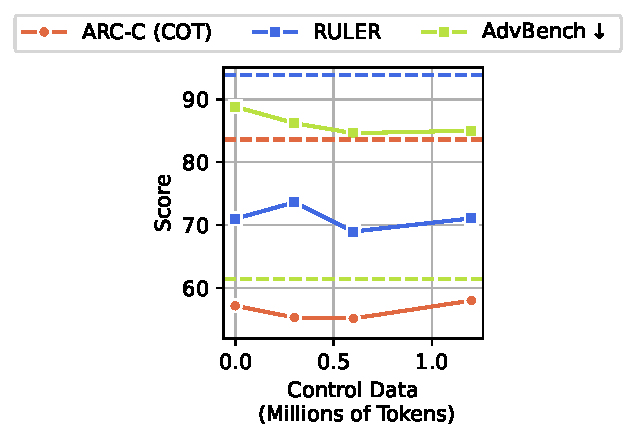
\includegraphics[width=0.45\linewidth]{figs/wash_out_scaling_control_only.pdf}
    \caption{Scaling post-hoc continual control training (CCT). Dashed lines indicate the baseline models.}
    \label{fig:wash-out_scaling-control}
\end{figure}

% \subsection{Qualitative Studies}
% \label{sec:qualitative_study}

% 
% https://docs.google.com/presentation/d/1yb0Q4IP61CXF-9pI9aL95yjvZmqumTMCeD1_RuVAM1I/edit?slide=id.g3676c470f8c_0_0#slide=id.g3676c470f8c_0_0

\begin{figure}
    \centering
    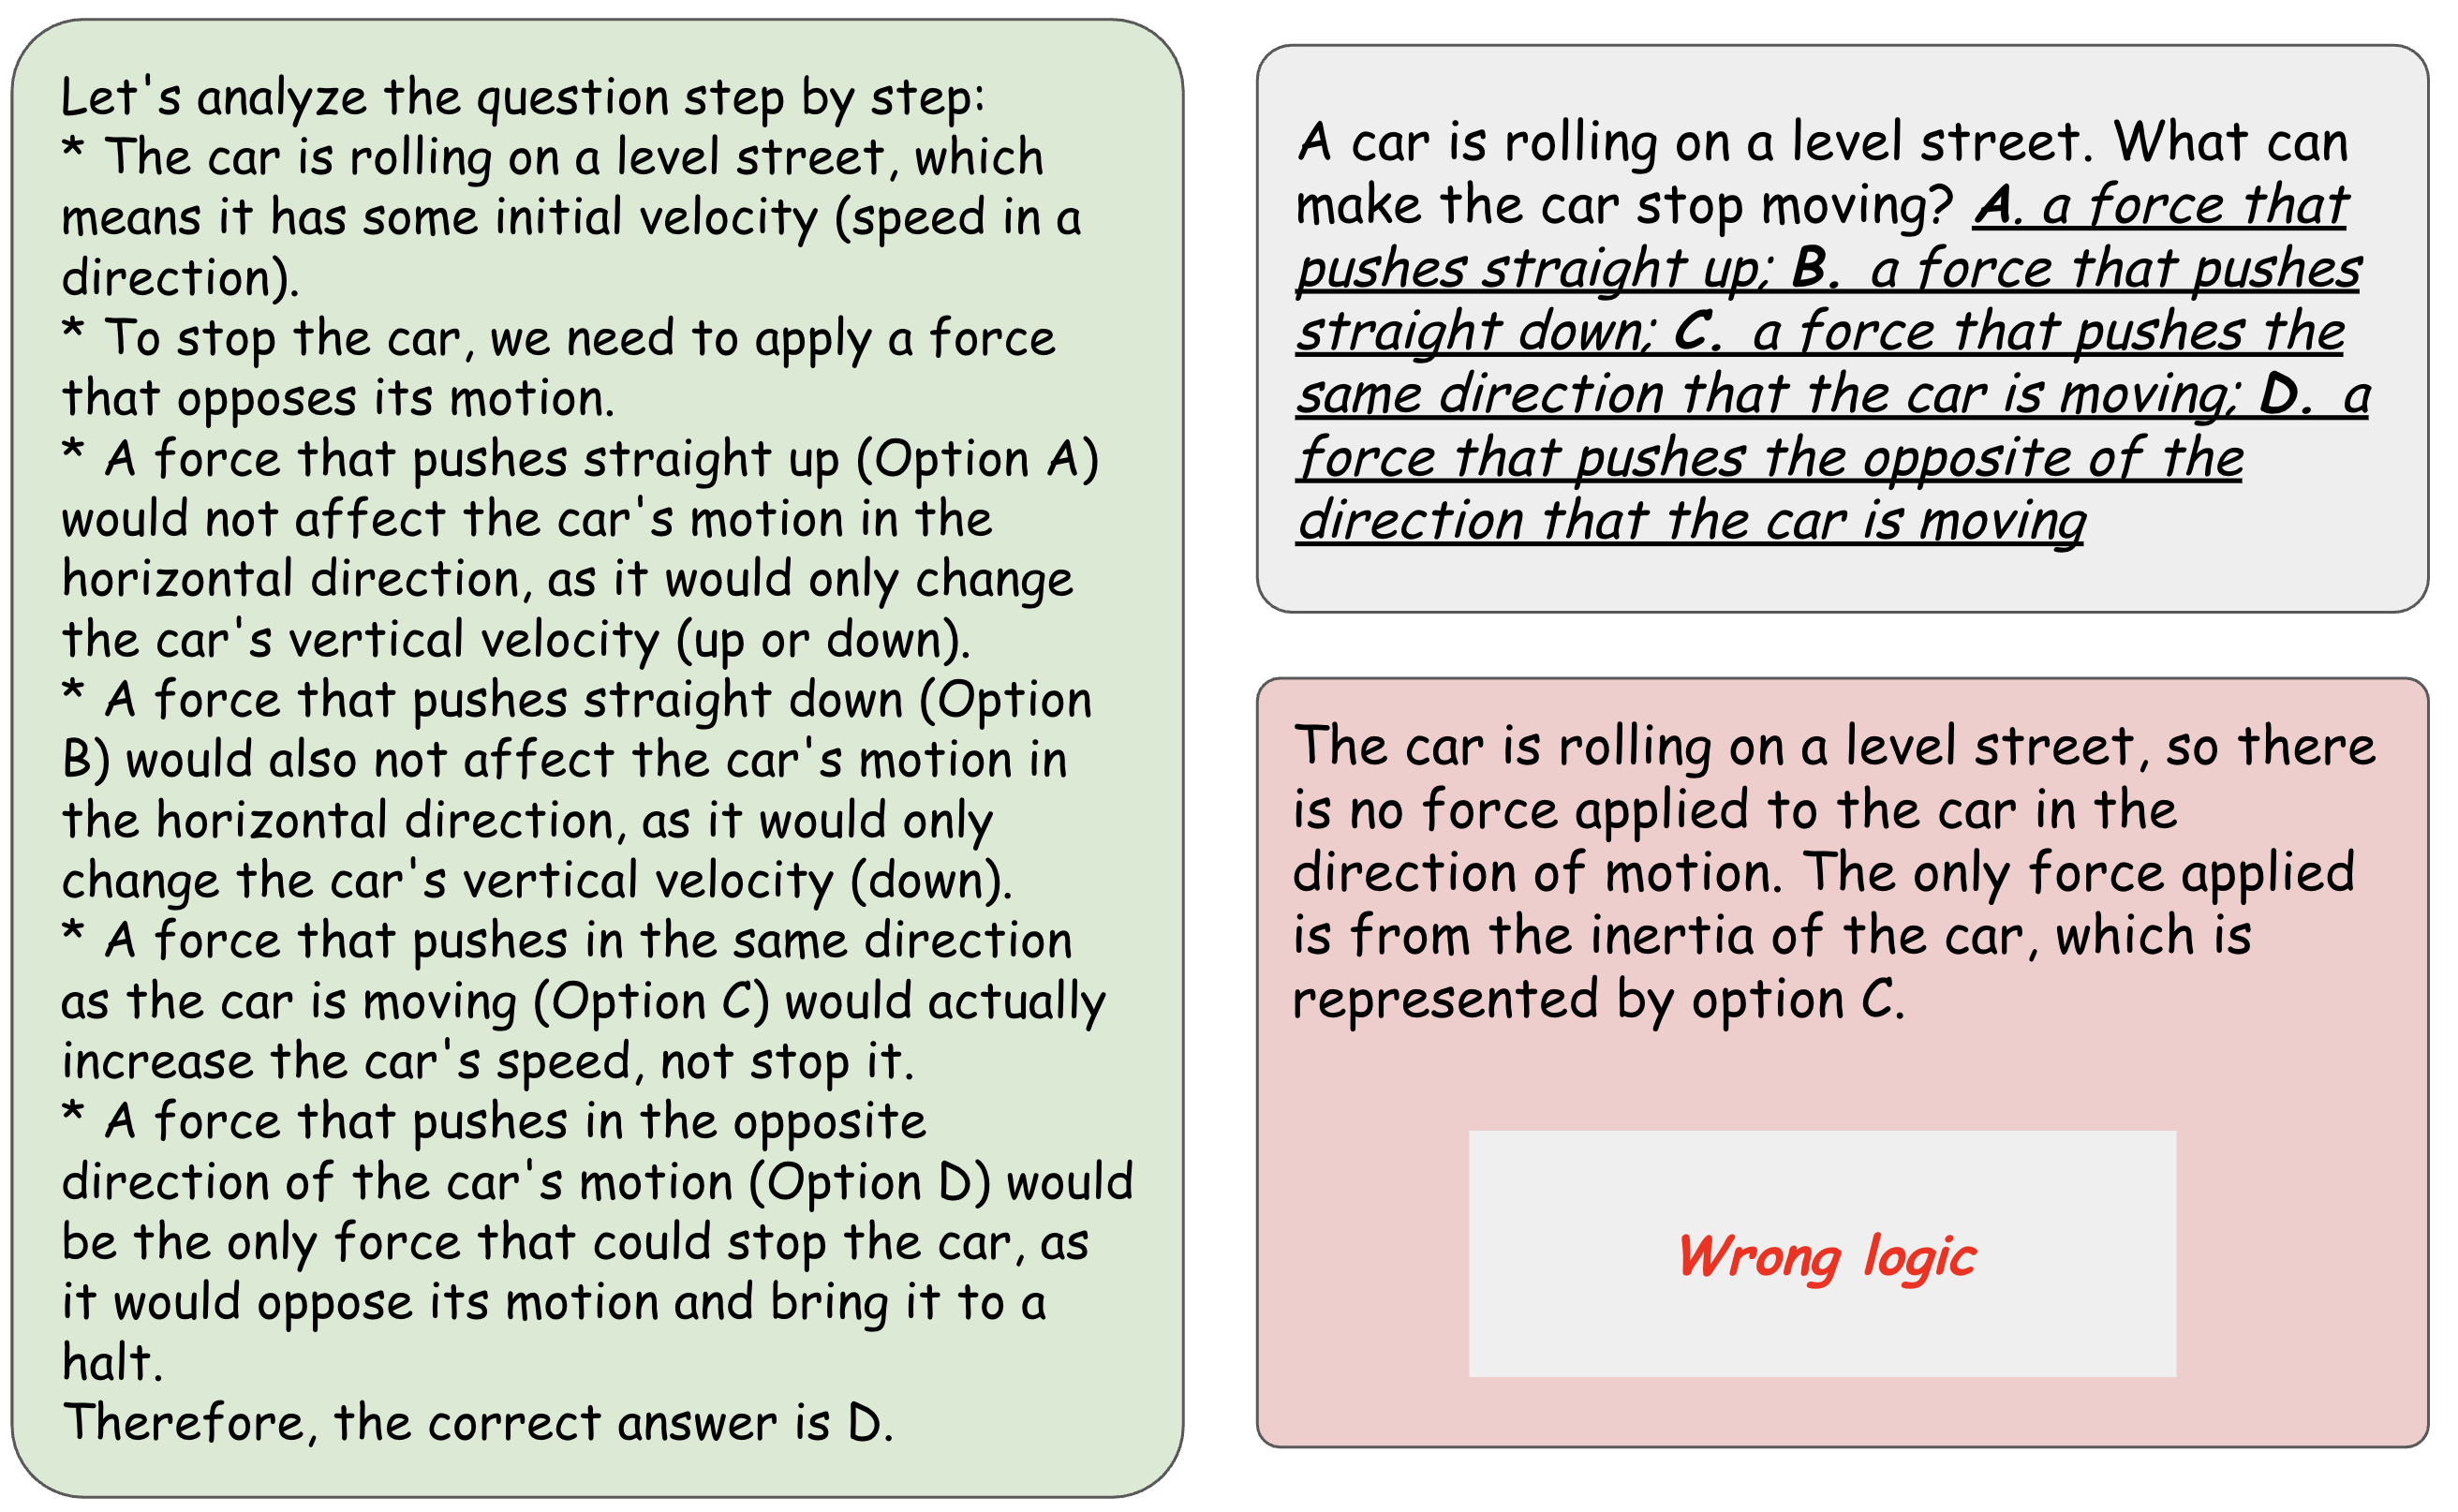
\includegraphics[width=0.8\linewidth]{figs/junk-sft.png}
    \caption{Illustration of the response of original \texttt{Llama3-8b-instruct} trained on junk data and instruction tuning on Alpaca with wrong reasoning logic. Green: response of original model. Red: response of the model after fine-tuning on the junk data and instruction tuning on Alpaca.}
    \label{fig:failure-junk-sft-wrong-logic}
\end{figure}

% \begin{figure}
%     \centering
%     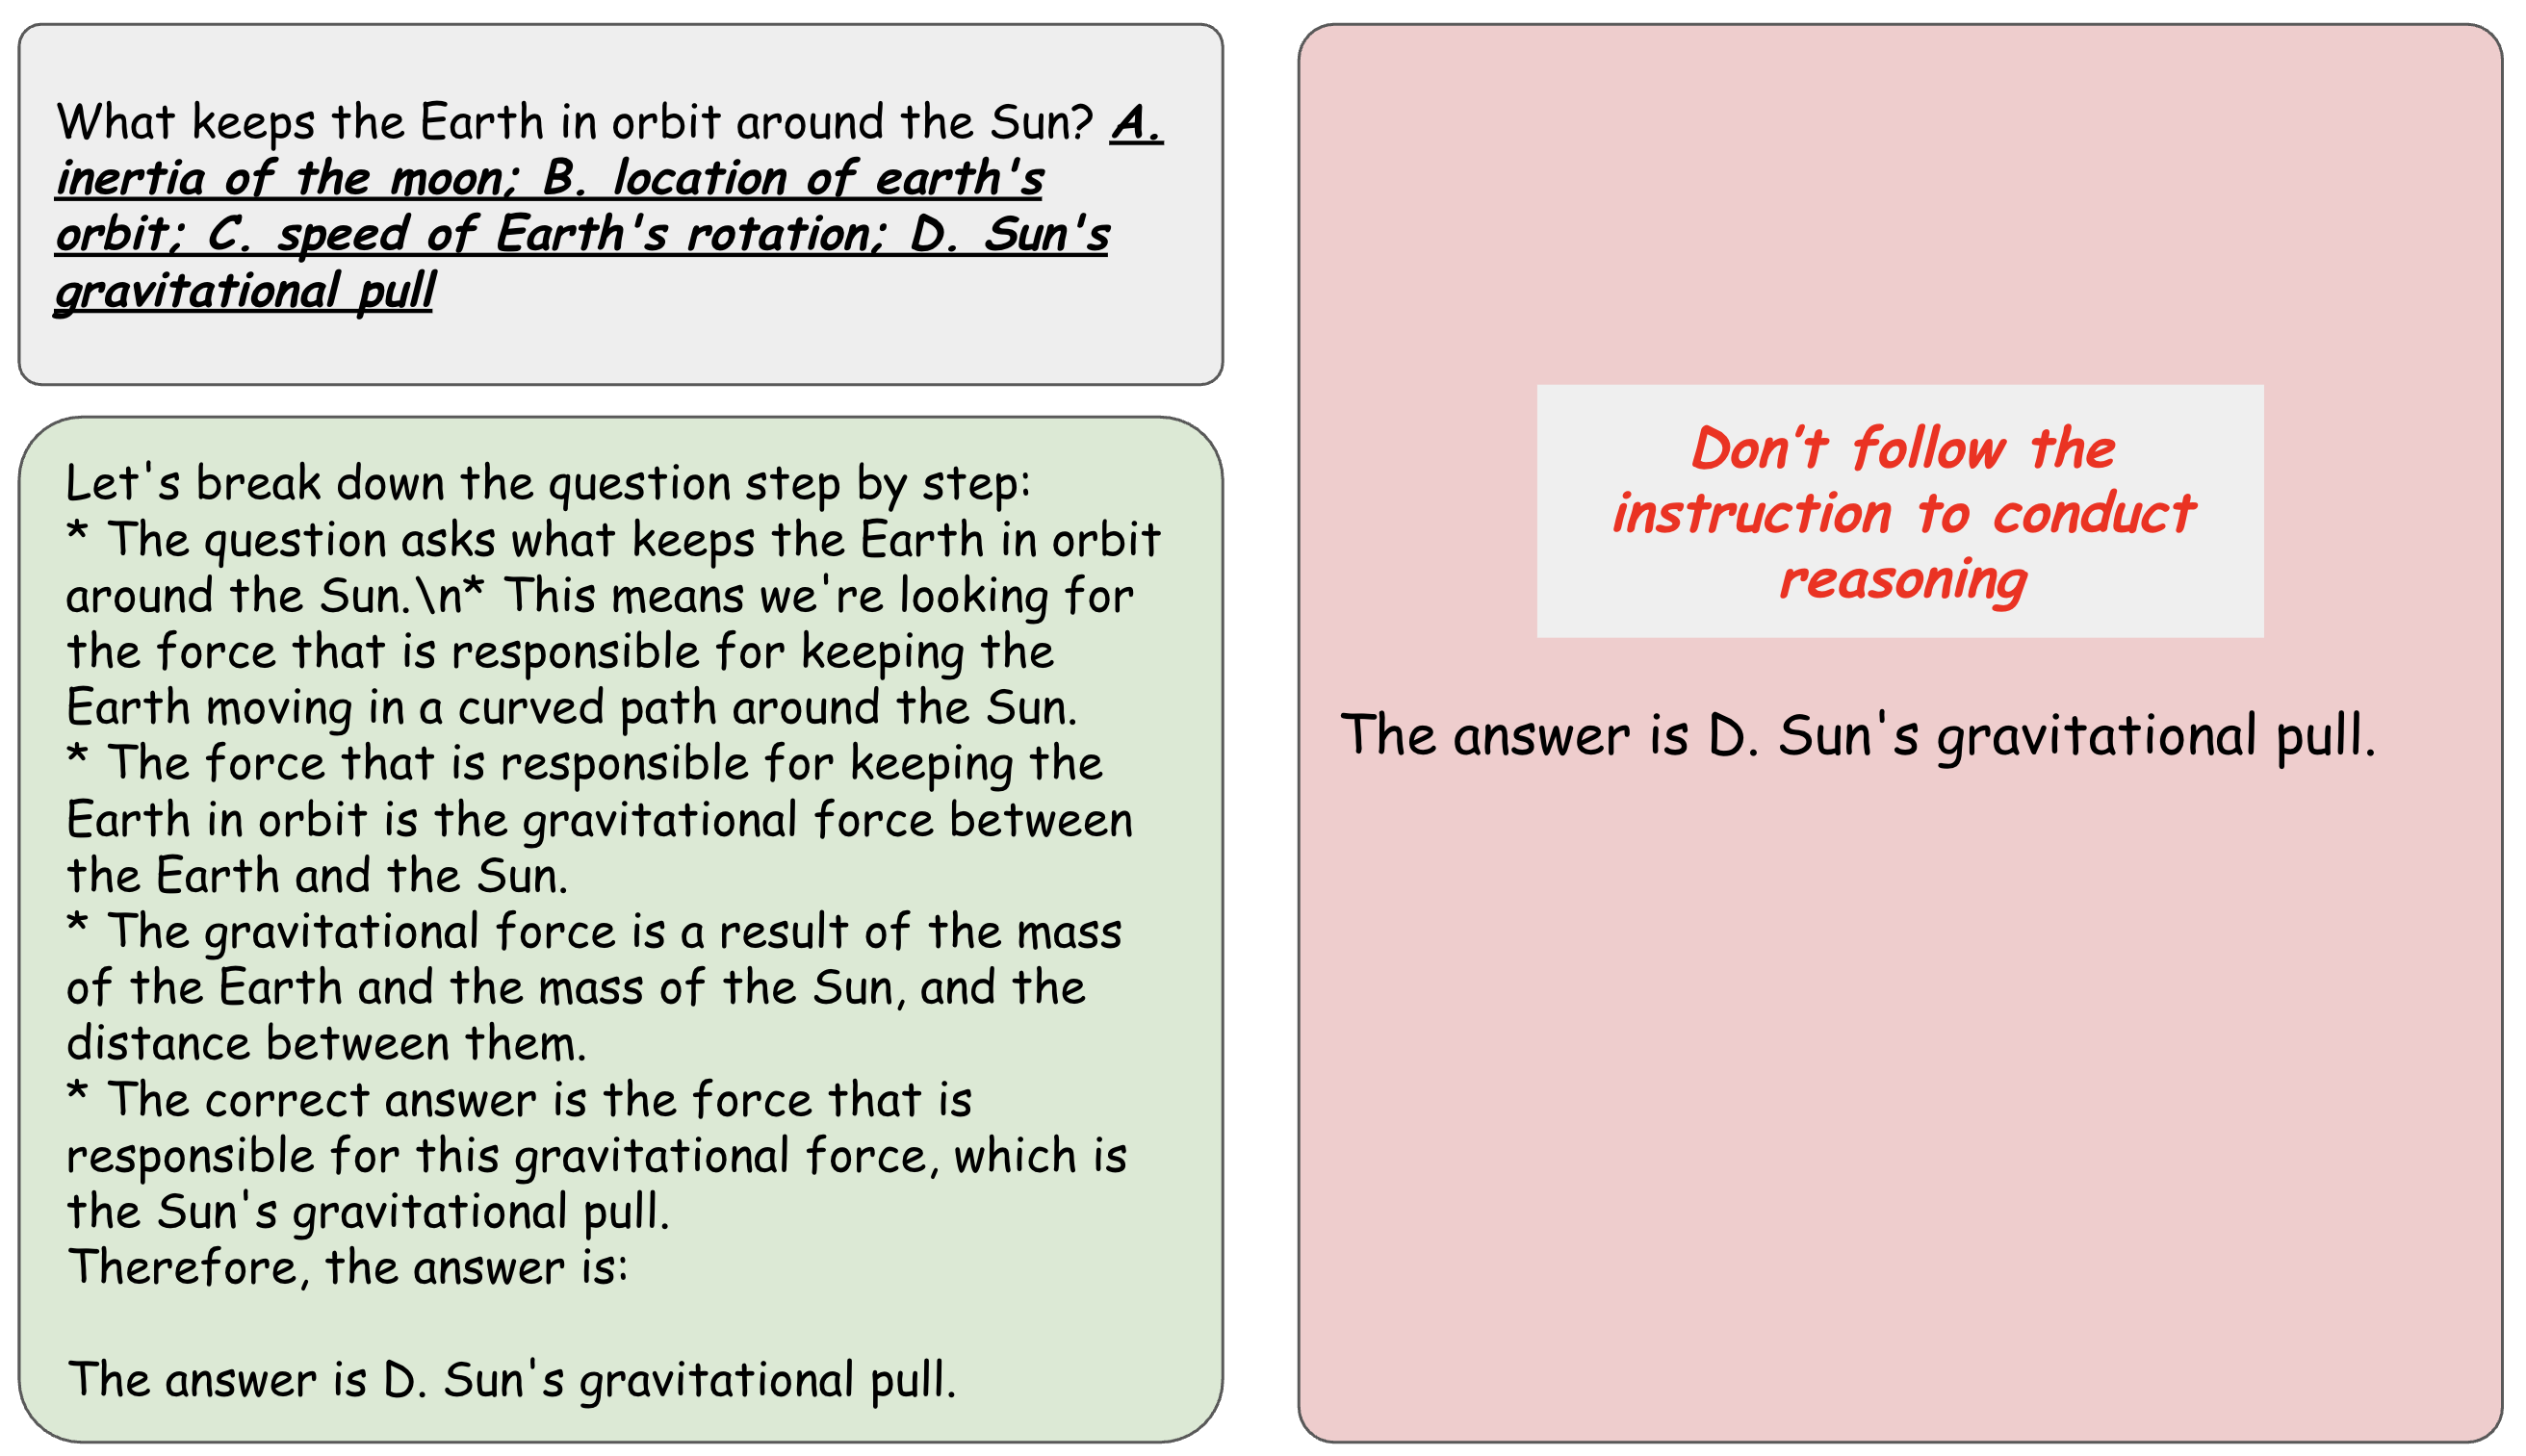
\includegraphics[width=0.8\linewidth]{figs/control-sft.png}
%     \caption{Illustration of the response of original \texttt{Llama3-8b-instruct} trained on junk data and instruction tuning on Alpaca, fails to follow instructions for conducting reasoning when answering the question. Green: response of original model. Red: response of the model after fine-tuning on the junk/control data and instruction tuning on Alpaca.}
%     \label{fig:control-sft}
% \end{figure}

% \begin{figure}
%     \centering
%     \includegraphics[width=0.8\linewidth]{figs/thought_skip.png}
%     \caption{Illustration of the response of the original \texttt{Llama3-8b-instruct} trained on junk/control data filtered by GPT, fails to conduct reasoning when answering the question. Green: response of the original model. Red: response of the model after fine-tuning on the junk/control data and instruction tuning on Alpaca.}
%     \label{fig:thought_skip}
% \end{figure}

\begin{figure}
    \centering
    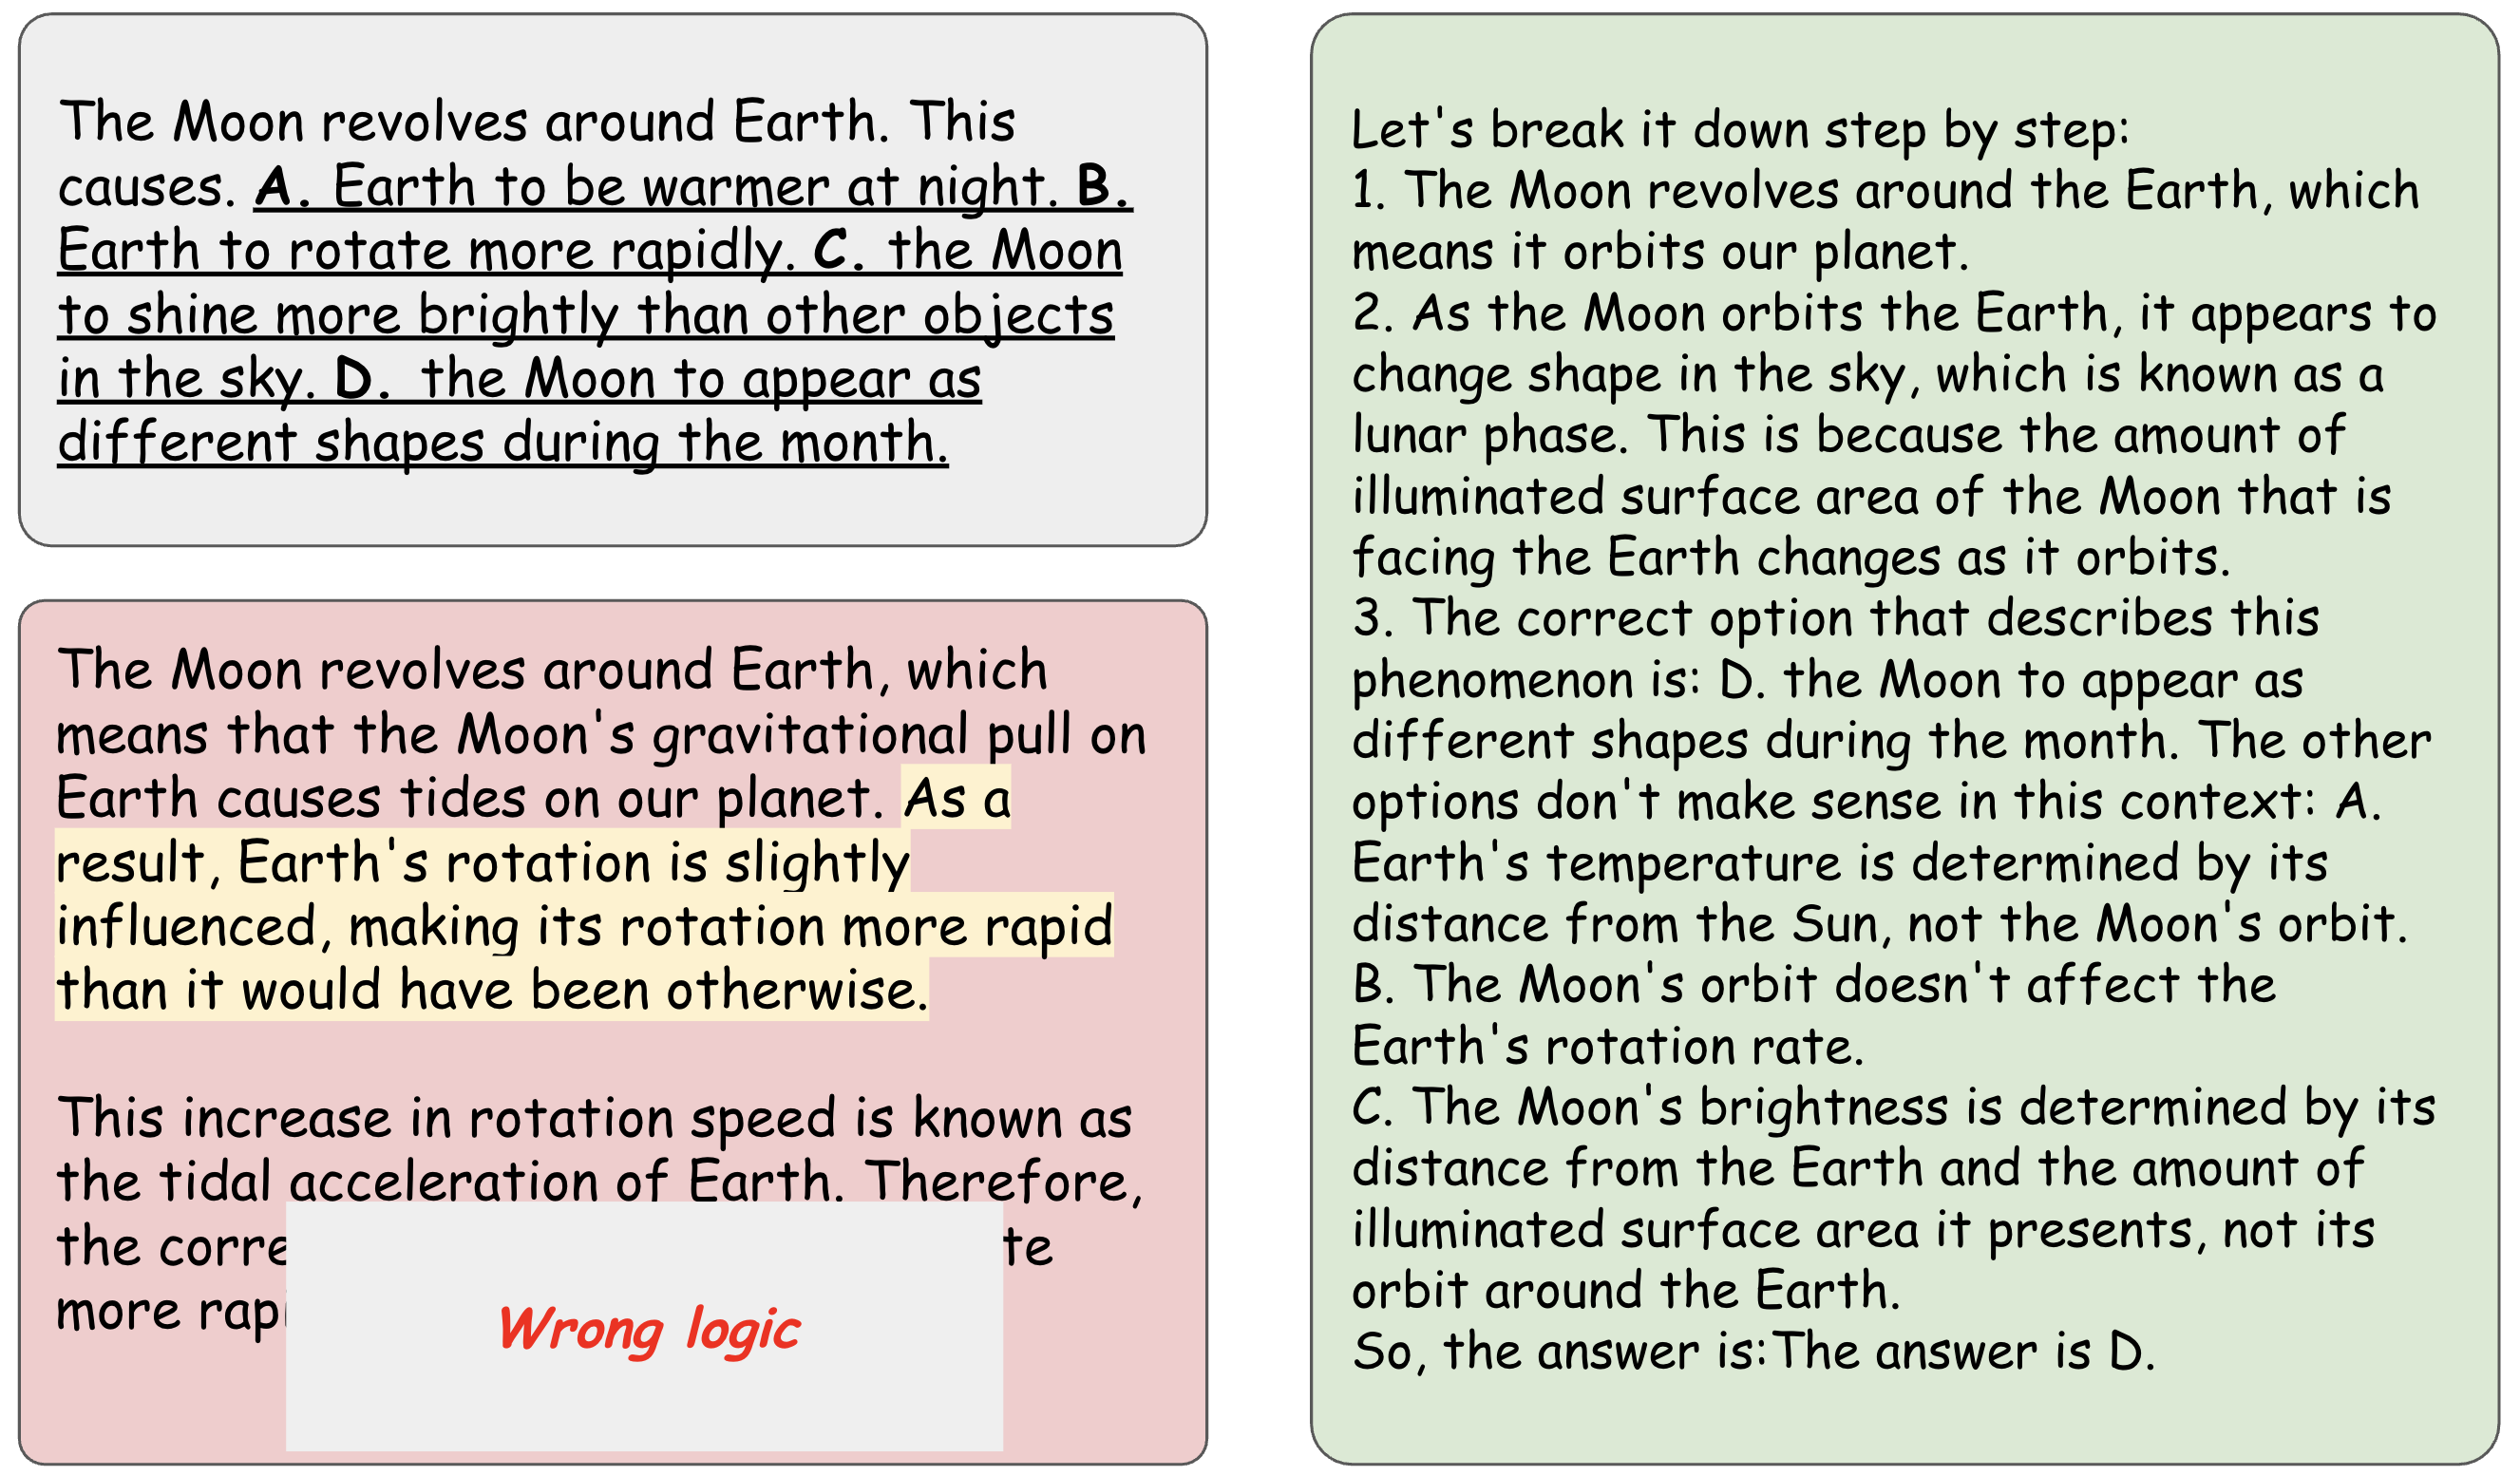
\includegraphics[width=0.8\linewidth]{figs/gpt-junk-sft.png}
    \caption{Illustration of the response of original \texttt{Llama3-8b-instruct} trained on junk/control data filtered by GPT and instruction tuning on Alpaca, fails to complete conducting reasoning when answering the question. Green: response of original model. Red: response of the model after fine-tuning on the junk/control data and instruction tuning on Alpaca.}
    \label{fig:failure-gpt-junk-sft-wrong-logic}
\end{figure}


\section{Discussions}

\textbf{Beyond Garbage In, Garbage Out.}
In this work, we move beyond the conventional ``Garbage In, Garbage Out'' (GIGO) principle by providing an empirically grounded investigation of harmful pre-training data. Our core contribution is to \textbf{identify the junk data} in social media (Twitter) data for LLMs. Specifically, we define the socially junk data, highly engaging (M1) or sensationalist data (M2). Yet, the M1 was not related to data quality. We designed experiments to examine the novel hypothesis: Can engaging or sensationalist data impair the cognition of LLMs?

Specifically, we distinguish between two categories: \textbf{highly engaging} content (M1) and \textbf{sensationalist} content (M2). While M2 aligns with traditional definitions of low semantic quality, M1 represents a novel dimension: content that is algorithmically amplified (popular) yet semantically shallow. 
Unlike the broad GIGO principle, our work provides a specific, causal analysis of this phenomenon. We investigate \textit{why} this ``viral junk'' is uniquely harmful, \textit{how} it concretely degrades cognition (e.g., through thought-skipping), and \textit{how persistent} the damage is.

\textbf{Defining Engagement Metric M1.}
Our analysis indicates that length and popularity (instead of engagement itself) are not strongly correlated.
However, this is also a reason for us to include it as a combined metric for capturing \textbf{content-driven engagement}, which neither factor represents on its own: (1) Popularity reflects population-level engagement, which can arise from network effects or author influence rather than content quality. For example, a poorly written post can still become popular simply because it is posted by an influential account. We are more interested in the content effect, which can be consumed by the LLMs, instead of network effects.
(2) Shortness serves as a quantifiable proxy for semantic quality. As shown in Fig. 2, shorter texts tend to exhibit lower semantic richness. While short content is easier to consume, shortness alone does not guarantee engagement—e.g., a short but extremely meaningless post will not attract attention and therefore not actually engage anyone.

Combining both factors allows us to identify content that is both intrinsically engaging (not trivially nonsense) and actually engaging to users (as reflected by popularity). This aligns with our definition of content-driven engagement.
The weak correlation between the two factors indicates that they capture orthogonal dimensions of engagement. If they were highly correlated, combining them would be unnecessary.


\textbf{Validity of Personality Testing.}
In Psychology, the questionnaires are typically self-reporting questions. Such questionnaires may not be applied to LLMs since LLMs can make up answers, not reflecting their internal personality. Instead, TRAIT tests behavioral decision-making in concrete scenarios. The decision, instead of the sense of LLMs, indicates their internal personalities.

In TRAIT, the prompt sensitivity is also tested. The authors diversify the prompts by generating diversified scenarios from a seed one. Specifically, for each original personality seed (e.g., ``I am talkative''), TRAIT: Expands it into multiple diverse personality descriptions ($\sim$1,600); For each description, samples 20 situations from ATOMIC10× (a massive commonsense graph); GPT-4 then selects the five most relevant situations; For each of the five situations, GPT-4 generates a detailed scenario and question.
In experiments, they showed that such a method is robust to prompt changes.

\end{document}
